\documentclass{article}
\usepackage{graphicx}
\usepackage{hyperref}
\usepackage[a4paper, total={7in, 10in}]{geometry} %6,10
\usepackage{float}
\usepackage[utf8]{inputenc}
\usepackage{listings}
\usepackage{xcolor}
\usepackage{amsmath}
\usepackage{amssymb}
\usepackage{multicol}
\usepackage{enumerate}
\usepackage{tikz}
\usepackage{mathtools}
\usepackage{array}
\usepackage{color, soul}
\usepackage{bbm}
\usetikzlibrary{positioning}
\DeclareMathOperator{\Tr}{Tr}
\newcommand*{\horzbar}{\rule[.5ex]{2.5ex}{0.5pt}}    % horizontal bar in matrices

\newcommand\undermat[2]{%
  \makebox[0pt][l]{$\smash{\underbrace{\phantom{%
    \begin{matrix}#2\end{matrix}}}_{\text{$#1$}}}$}#2}



\title{
    \includegraphics[scale=0.6]{../images/LogoPoli2.jpg}\\[2cm]
    \huge{\textsc{Numerical Analysis for Machine Learning}}
    \author{\Large{\textsc{Lorenzo Bozzoni}}}
  \date{\today}}




\begin{document}
%\begin{vplace}[0.7]
%  \maketitle
%\end{vplace}

\maketitle
\newpage
\tableofcontents

\section{Basic concepts of linear algebra}
The following are the main concepts of linear algebra we are going to face during the starting phase of the course:
\begin{enumerate}
    \item Linear systems of equations: $A\underline{x} = \underline{b}$
    \item Eigenvalues and eigenvectors: $A\underline{x} = \lambda \underline{x}$
    \item Singular value decomposition (SVD):$A\underline{v} = \sigma u$
    \item Minimization problem
    \item Factorization: $PA = LU$
\end{enumerate}


% $\mathbb{A}\underline{x} = \lambda \underline{x}$
% $\mathbb{A}\underline{v} = \sigma \mathbb{u}$

\section{Matrix-vector multiplication}
\[
\underline{c} = \underbrace{\begin{bmatrix}
    1 & 2\\
    3 & 4\\
    5 & 6
\end{bmatrix}}_{A_1}
\underbrace{\begin{bmatrix}
    x_1\\
    x_2
\end{bmatrix}}_{\underline{x}}
= 
\begin{bmatrix}
    1x_1 + 2x_2\\
    3x_1 + 4x_2\\
    5x_1 + 6x_2 
\end{bmatrix}
=
\underbrace{
\begin{bmatrix}
    1\\
    2\\
    3
\end{bmatrix}
x_1+
\begin{bmatrix}
    4\\
    5\\
    6
\end{bmatrix}
x_2
}_{\text{linear combination}}
\]
We say that the vector $\underline{c}$ belongs to the \textbf{column space} of $A_1$, i.e. $\underline{c} \in \mathcal{C}(A_1)$.
\[
\overbrace{
\underbrace{
\begin{bmatrix}
    1 & 4 & 7\\
    2 & 5 & 8\\
    3 & 6 & 9
\end{bmatrix}}_{\underline{a_1} \hspace{0.2cm} \underline{a_2} \hspace{0.2cm} \underline{a_3}}
}^{A_2}
\begin{bmatrix}
    x_1\\
    x_2\\
    x_3
\end{bmatrix}
\]
In this case we can easily notice that $\underline{a_3} = \underline{a_1} + \underline{a_2}$, which means that one column can be expressed as a linear combination of the other two (this means that the matrix $A_2$ is singular). Because of this, we can say that $\mathcal{C}(A_2) = \mathcal{C}(A_1)$, i.e. the column space of $A_2$ is the same as the column space of $A_1$.

Those columns spaces are a plane passing through the origin and spanned by the two vectors $\underline{a_1}$ and $\underline{a_2}$ (they define the slope of that plane).

Let's now consider these matrix:
\[
\underbrace{
\begin{bmatrix}
    1 & 4 & 7\\
    2 & 5 & 8\\
    3 & 6 & 10
\end{bmatrix}
}_{A_3} 
\hspace{3cm}
\underbrace{
\begin{bmatrix}
    1 & 2 & 3\\
    2 & 4 & 6\\
    3 & 6 & 9
\end{bmatrix}
}_{A_4} 
\]
This left-hand matrix column space is $\mathcal{C}(A_3) = \mathbb{R}^3$, i.e. the entire real space of three dimensions. This is because the three vector columns of $A_3$ are linearly independet so they span the entire space and not just a plane.
While the column space of $A_4$ is instead: $\mathcal{C}(A_3) = \begin{bmatrix}
    1&2&3
\end{bmatrix}^T$ i.e. just a line since the three columns are linearly dependent and so they lie on the same line (they are parallel) just with different magnitude.

Another measure regarding matrices is the \textbf{dimension} or \textbf{rank}:
\begin{itemize}
    \item $rank(A_1) = 2$
    \item $rank(A_2) = 2$
    \item $rank(A_3) = 3$
    \item $rank(A_4) = 1$
\end{itemize}
The rank is the number of linearly independent columns (or rows) of a matrix.

Let's consider again the matrix $A_3$:
\[
\begin{bmatrix}
    1 & 4 & 7\\
    2 & 5 & 8\\
    3 & 6 & 10
\end{bmatrix}
\begin{bmatrix}
    x_1\\
    x_2\\
    x_3
\end{bmatrix}
= 
\underbrace{\begin{bmatrix}
    1\\
    2\\
    3
\end{bmatrix}
x_1+
\begin{bmatrix}
    4\\
    5\\
    6
\end{bmatrix}
x_2+
\begin{bmatrix}
    7\\
    8\\
    10
\end{bmatrix}
x_3}_{\in \mathcal{C}(A_3)}
=
\begin{bmatrix}
    b_1\\
    b_2\\
    b_3
\end{bmatrix}
\]
so $\underline{b}$ must be in $\mathcal{C}(A_3)$ in order to have the system solvable. If $\underline{b} \notin \mathcal{C}(A_3)$, then the system is not solvable. In this particular case we have that the columns of $A_3$ are linearly independent, so the system is solvable for any $\underline{b}$ because $\mathcal{C}(A_3) = \mathbb{R}^3$ and so $\underline{b}$ is for sure inside that space. \\

Given A, find $\mathcal{C}(A)$. How can we solve this problem? Considering $\underline{a_1}, \dots, \underline{a_n}$ as A columns, we can use the following iterative algorithm:
\begin{itemize}
    \item put $\underline{a_1}$ in $\mathcal{C}(A)$
    \item if $\underline{a_2} = \alpha \underline{a_1} \rightarrow \underline{a_2} \notin \mathcal{C}(A)$, otherwise put $\underline{a_2}$ in $\mathcal{C}(A)$
\end{itemize}
Until you reach the last column.

\subsection{Row-reduced echelon form}
Given the matrix $A$, defined as follow:
\[
A = \begin{bmatrix}
    1 & 4 & 7\\
    2 & 5 & 8\\
    3 & 6 & 9
\end{bmatrix}
\]
we can obtain the \textbf{row-reduced echelon form} of $A$ by applying the following operations:
\[
A = CR = \begin{bmatrix}
1 & 4\\
2 & 5\\
3 & 6
\end{bmatrix}
\begin{bmatrix}
    1 & 0 & -1\\
    0 & 1 & 2
\end{bmatrix}
\]
where $C$ is the matrix containing the columns of $A$ that are linearly independent (i.e. $\mathcal{C}(A)$) and $R$ is the matrix of the coefficients of the linear combination of the columns of $A$ that gives the columns of $C$.\\

Let's now consider the following matrix:
\[
A_1 = \begin{bmatrix}
1 & 4\\
2 & 5\\
3 & 6
\end{bmatrix}  
\hspace{2cm}
A_1^\intercal = \begin{bmatrix}
1 & 2 & 3\\
4 & 5 & 6
\end{bmatrix}  
\]
What we can say about $A_1^\intercal$ column space? Is there any relationship with the column space of $A_1$?

In order to compute its column space, we can start noticing that: $\underline{a_3} = 2\underline{a_2} - \underline{a_1}$. So, in general, we can say that:
\[
dim(\mathcal{C}(A)) = dim(\mathcal{C}(A^\intercal)) = r \leq n \hspace{1cm} \text{where $n$ is the number of columns of $A$}
\]

\section{Matrix-matrix multiplication}
\[
C = AB = \begin{bmatrix}
    \vline & \vline & \vline\\
    \underline{a_1} & \ldots & \underline{a_n}\\
    \vline & \vline & \vline
\end{bmatrix}
\begin{bmatrix}
    \horzbar & \underline{b_1} & \horzbar\\
    \horzbar & \vdots & \horzbar\\
    \horzbar & \underline{b_n} & \horzbar
\end{bmatrix}
= \overset{\overset{\text{col}}{\downarrow}}{\underline{a_1}}\overset{\overset{\text{row}}{\downarrow}}{\underline{b_1}} + \dots + \underline{a_n}\underline{b_n}
\] 
All the products that are summed at the end of the equation are matrices of rank 1. 

Example:
\[
\begin{bmatrix}
1 & 2\\
3 & 4
\end{bmatrix}  
\begin{bmatrix}
    2 & 1\\
    2 & 3
\end{bmatrix}
= \underbrace{
    \begin{bmatrix}
        2 & 1\\
        6 & 3
    \end{bmatrix}
}_{\text{rank = 1}}
+ \underbrace{
    \begin{bmatrix}
        4 & 6\\
        8 & 12
    \end{bmatrix}
}_{\text{rank = 1}}
= \begin{bmatrix}
    6 & 7\\
    14 & 15
\end{bmatrix}
\]


\section{Factorizations}
\begin{enumerate}
    \item $A = LU$ or $PA = LU$
    \item $A = QR$ where $Q$ is orthogonal and $R$ is upper triangular
    This is an improved version of the Row-reduced echelon form because that worked only for square matrices, while this works for any matrix.
    \item Eigenvalues and eigenvectors decomposition: when $S = S^\intercal$ (symmetric matrix) we can factorize it as $S = Q\Lambda Q^\intercal$ where $\Lambda$ is a diagonal matrix and $Q$ is an orthogonal matrix (they are all squared matrices)
    \item Generalization of the above: $A = X\Lambda X^{-1}$ where $X$ is a non-orthogonal matrix
    \item $A = U\Sigma V^\intercal$ where $U$ and $V$ are orthogonal matrices and $\Sigma$ is a pseudo-diagonal matrix
\end{enumerate}
A matrix is said to be pseudo-diagonal if it has the following form:
\[
    \Sigma = 
    \begin{bmatrix}
        \sigma_1 & 0 & 0 & 0\\
        0 & \sigma_2 & 0 & 0\\
        0 & 0 & \ddots & 0\\
        0 & 0 & 0 & \sigma_n\\
        0 & 0 & 0 & 0\\
        \vdots & \vdots & \vdots & \vdots\\
        0 & 0 & 0 & 0
    \end{bmatrix}
    \hspace{2cm}
    m \text{ rows} \times n \text{ columns}
\]
So it has diagonal elements for the first $n$ rows then it has all zeros.

\subsection{Orthogonal matrices}
A matrix $Q$ is orthogonal if $Q^\intercal Q = I$ (i.e. $Q^\intercal = Q^{-1}$). This means that the columns of $Q$ are orthonormal, i.e. they are orthogonal and have unit norm.\\

The determinant of a orthogonal matrix is $\pm 1$.

Properties:
\begin{itemize}
    \item $||Q\underline{x}|| = ||\underline{x}||$
    \item $||Q\underline{x}||^2 = (Q\underline{x})^\intercal Q\underline{x} = \underline{x}^\intercal \underbrace{Q^\intercal Q}_{I} \underline{x} = ||\underline{x}||^2$
\end{itemize}
The first property is particularly easy to interpret since it means that when we multiply an orthogonal matrix to a vector, the norm of the vector doesn't change. As a proof of this, we can consider the following examples:

\subsubsection{Rotation}
A classical rotation matrix is:
\[
\begin{bmatrix}
    cos(\theta) & -sin(\theta)\\
    sin(\theta) & cos(\theta)
\end{bmatrix}    
\]
\subsubsection{Reflection}
\begin{center}
    \includegraphics[scale=0.5]{images/Reflection.png}
\end{center}
The horizontal line in the figure represent a plane $\pi$ while $\underline{n}$ is its normal vector of length 1. 
Given $\underline{v}$ to obtain $\underline{w}$ we can use the following formula:
\[
\underline{w} = \underline{v} - 2(\underline{v}^\intercal \underline{n})\underline{n} = \underbrace{(I - 2\underline{n}\underline{n}^\intercal)}_{\text{reflection matrix}}\underline{v}
\]
Moreover, the reflection matrix $R$ is not only orthogonal, but also the inverse of itself, i.e. $R^{-1} = R^\intercal$. This makes sense because if we apply the reflection matrix twice, we obtain the original vector $\underline{v}$, i.e. the reflection of the reflection is the starting vector.

If we didn't have the 2 in the formula, we would obtain the projection of $\underline{v}$ on the plane $\pi$ which is called orthogonal projection and the matrix $R$ would be singular. \\

Let's now dive a bit into the third point of the factorization list. We said that when $S = S^\intercal$ (symmetric matrix) we can factorize it as $S = Q\Lambda Q^\intercal$ where $\Lambda$ is a diagonal matrix and $Q$ is an orthogonal matrix.\\
\[
S = S^\intercal = \underbrace{(Q\Lambda))}_{\tilde{Q}}Q^\intercal = \tilde{Q}Q^\intercal   
\]
\[
\tilde{Q} = \underline{q_1}\underline{\lambda_1} + \dots + \underline{q_n}\underline{\lambda_n}    
\]
Where the $q$ vectors are columns and $\lambda$ vectors are rows.
So we can reformulate:
\[
    S = (\underline{q_1}\underline{\lambda_1} + \dots + \underline{q_n}\underline{\lambda_n})Q^\intercal = \underline{q_1}\underline{\lambda_1}\underline{q_1}^\intercal + \dots + \underline{q_n}\underline{\lambda_n}\underline{q_n}^\intercal
\]
This is called \textbf{spectral decomposition} of matrix $S$ and $q_1, \dots, q_n$ are the eigenvectors of $S$ while $\lambda_1, \dots, \lambda_n$ are the eigenvalues of $S$.
\[
    S\underline{q_1} = \lambda_1\underline{q_1} = (\underline{q_1}\underline{\lambda_1}\underline{q_1}^\intercal + \dots + \underline{q_n}\underline{\lambda_n}\underline{q_n}^\intercal)\underline{q_1} = 
    \underline{\lambda_1}\underline{q_1}(\underline{q_1^\intercal}\underline{q_1})
    \]
All the other products are null since the vector $\underline{q_1}$ is orthogonal to all the other vectors $\underline{q_i}$ for $i \neq 1$ (recall that they are eigenvectors).

\section{Null spaces}
Let's consider the starting problem for a linear system of equations:
\[
A\underline{x} = \underline{b} \hspace{1cm} \text{with} \hspace{1cm} A\in \mathbb{R}^{m \times n}, \text{rank($A$)}=r    
\]

We are going to introduce 2 more spaces other than the column ones. To do so we consider:
\[
  A\underline{x} = \underline{0} \hspace{1cm} \rightarrow \hspace{1cm} N(A) \equiv \ker(A) = \{\underline{x} \in \mathbb{R}^n : A\underline{x} = \underline{0}\}  
\]
\[
    A^\intercal\underline{x} = \underline{0} \hspace{1cm} \rightarrow \hspace{1cm} N(A^\intercal) \equiv \ker(A^\intercal) = \{\underline{x} \in \mathbb{R}^n : A^\intercal\underline{x} = \underline{0}\}    
\]

So now, adding the so called \textbf{null spaces} we have that:
\begin{enumerate}
    \item $\mathcal{C}(A) \subset  \mathbb{R}^m$ and $dim(\mathcal{C}(A)) = r$
    \item $\mathcal{C}(A^\intercal) \subset \mathbb{R}^n$ and $dim(\mathcal{C}(A^\intercal)) = r$
    \item $N(A) \subset \mathbb{R}^n$ and $dim(N(A)) = ?$
    \item $N(A^\intercal) \subset \mathbb{R}^m$ and $dim(N(A^\intercal)) = ?$
\end{enumerate}
We still do not know the dimensions of those spaces. \\

\textbf{Example}\\
\[
A = \begin{bmatrix}
    1 & 4 & 7\\
    2 & 5 & 8\\
    3 & 6 & 9
\end{bmatrix}
\begin{bmatrix}
    x_1\\
    x_2\\
    x_3
\end{bmatrix}
= 
\begin{bmatrix}
    0\\
    0\\
    0
\end{bmatrix}
\hspace{0.3cm} \implies \hspace{0.3cm}
\begin{cases}
    x_1 + 4x_2 + 7x_3 = 0\\
    2x_1 + 5x_2 + 8x_3 = 0\\
    3x_1 + 6x_2 + 9x_3 = 0
\end{cases}    
\]
We compute the first equation
\[
    x_1 = -4x_2 - 7x_3 \hspace{0.3cm} \implies \hspace{0.3cm} \begin{cases}
        -3x_2 - 6x_3 = 0\\
        -6x_2 - 12x_3 = 0
    \end{cases}
\]
What is important to notice is that $A$ has rank$=2$ so we have $3-2=1$  \textbf{degrees of freedom}, i.e. we can choose one variable and the other two are automatically defined. This is visible in the last two equations of the system for example. 
In general, the degrees of freedom are given by $n-r$ where $n$ is the number of columns of $A$ and $r$ is the rank of $A$.\\

If we had 10 instead of 9 in $A$ we would have had $3-3=0$ degrees of freedom. This would translate in having the matrix $A$ full rank and $N(A) = \{\underline{0}\}$ so the only solution would be the null vector.


\section{Null space cardinality}
In the first lecture, we defined 4 spaces: $N(A), N(A^\intercal), \mathcal{C}(A), \mathcal{C}(A^\intercal)$. For the last two we defined also their cardinality whilst for the first ones we weren't able to tell yet. In this lecture we are going to find those values and prove them. In order to do so, we start from few useful properties:
\begin{enumerate}
    \item $\underline{x} = \underline{0} \in N(A)$ for any matrix $A$
    \item if $\underline{x}, \underline{y} \in N(A) \implies A(\underline{x} + \underline{y}) = \underline{0}$
    \item if $\underline{x} \in N(A) \implies \alpha\underline{x}$ with $\alpha \in \mathbb{R} \implies A(\alpha\underline{x}) = \underline{0}$
\end{enumerate}  

Consider, once again, the matrix $A \in \mathbb{R}^{m\times n}$, rank($A$) = $r \leq n$. 
We have seen the decomposition $A = CR$, where $C$ contains the linearly independent columns of $A$ and $R$ contains the coefficients that allow to recover the columns of $A$ starting from its independent columns. 
So, the matrix $A$ can be rewritten as:
\[
  A = \begin{bmatrix}
    A_1 & A_2
  \end{bmatrix} 
  \hspace{1cm}
  A_1 \in \mathbb{R}^{m\times r} \hspace{1cm} A_2 \in \mathbb{R}^{m\times (n-r)} 
\]
Where $A_1$ contains the independent columns of $A$ and $A_2$ the dependent ones.
Example:
\[
A = 
\begin{bmatrix}
    1 & 4 & 7\\
    2 & 5 & 8\\
    3 & 6 & 9
\end{bmatrix}
= 
\underbrace{
\begin{bmatrix}
1 & 4\\
2 & 5\\
3 & 6
\end{bmatrix}}_{A_1}
\begin{bmatrix}
    1 & 0 & -1\\
    0 & 1 & \undermat{B}{2}
\end{bmatrix}
\]
Since we have the last column of $A$, that is linearly dependent so it belongs to $A_2$, we can reformulate it in this way:
\[
    A = \begin{bmatrix}
        A_1 & A_2
      \end{bmatrix} 
    = \begin{bmatrix}
        A_1 & A_1B
    \end{bmatrix}
\]
We build a new matrix $K$ defined as follows:
\[
    K = \begin{bmatrix}
        -B\\
        I_{n-r}
    \end{bmatrix}
    \hspace{1cm}
    K \in \mathbb{R}^{n\times(n-r)}    
    \hspace{1cm}
    B \in \mathbb{R}^{r\times(n-r)}    
\]

\[
AK = \begin{bmatrix}
    A_1 & A_1B
\end{bmatrix} 
\begin{bmatrix}
    -B\\
    I_{n-r}
\end{bmatrix}
= A_1(-B) + A_1B = 0   
\]
Where the last 0 is actually a matrix of zeros of dimension $m\times(n-r)$
because A has size $m\times n$ and $K$ has size $n\times(n-r)$.
We have that:
\[
    AK = 0 \implies A\underline{k_i} = 0 \hspace{1cm} \forall i \in \{1, \dots, n-r\}    
\]
Where $k_i$ is the i-th column of $K$. This means that: $\underline{k_i} \in N(A) \hspace{0.2cm} \forall i$.

Now, we want to demonstrate that: $K\underline{u} = 0 \implies \underline{u} = \underline{0}$. 
To do so, we start from expanding $K$ from its definition:
\[
    K = \begin{bmatrix}
        -B\\
        I
    \end{bmatrix}
    \underline{u} = 0
    \implies
    \begin{bmatrix}
        -B\underline{u}\\
        \underline{u}
    \end{bmatrix}
    = 
    \begin{bmatrix}
        \underline{0}\\
        \underline{0}
    \end{bmatrix}
\]
Where the two zero vectors have dimension $r$ and $n-r$ respectively! Considering the second row of the matrix we get: $\underline{u} = \underline{0}$ so all columns of $K$ are linearly independent.\\

If we consider the problem ($\star$) $A\underline{x} = \underline{0}$, we want to prove that each \underline{x} that satisfy ($\star$) must be a linear combination of the columns of $K$.\\
\[
    A_1\underline{x} = \underline{0} \in \mathbb{R}^m \implies \underline{x} = \underline{0} \in \mathbb{R}^r    
\]
Because $A_1$ has linearly independent columns, i.e. has full rank.
\[
    A\underline{u} = \underline{0} \in \mathbb{R}^m \implies \begin{bmatrix}
        A_1 & A_1B
    \end{bmatrix} 
    \begin{bmatrix}
        \underline{u_1}\\
        \underline{u_2}
    \end{bmatrix}  
    = 
    \begin{bmatrix}
        A_1\underline{u_1} + A_1B\underline{u_2}\\
    \end{bmatrix}
    = 
    A_1\left[\underline{u_1} + B\underline{u_2}\right]
    = \underline{0}
\]
We can notice that the last formulation obtained in the equation has the same form as the one from where we started the prove, so we can say that:
\[
    \underline{u_1} + B\underline{u_2} = \underline{0} \implies \underline{u_1} = -B\underline{u_2}    
\]
\[
   \underline{u} = \begin{bmatrix}
    -B\underline{u_2}\\
    \underline{u_2}
\end{bmatrix}
    =
\underbrace{\begin{bmatrix}
    -B\\
    I
\end{bmatrix}}_{K}
    \underline{u_2}
    = K\underline{u_2}
    \implies 
    dim(N(A)) = n - r
\]
\section{Eigenvalues and eigenvectors}
Start considering a generic square matrix $n \times n$. We are going later to discuss even the simmetry and positive definite properties.
Here below are the vectorial and the matrix form of the eigenvalue problem:
\[
    A\underline{x_i} = \lambda_i\underline{x_i} \hspace{0.5cm} i = 1, \dots, n \hspace{1cm} X^{-1}AX = \Lambda
\]
Where in the right-hand side there is a diagonal matrix $\Lambda$ with the eigenvalues of $A$ on the diagonal while the matrix $X$ with the eigenvectors of $A$ as columns.\\

\subsection{Eigenvectors of matrix power}
What can we say about the eigenvectors and eigenvalues of $A^2$?
\[
    A^2\underline{x_i} = A(A\underline{x_i}) = A(\lambda_i\underline{x_i}) = \lambda_i(A\underline{x_i}) = \lambda_i^2\underline{x_i}    
\]
So the eigenvalues of $A^2$ are the eigenvalues of $A$ squared.This is valid for any power of $A$ since this method can be applied recursively and it is very useful when there are problems in which a matrix is iteratively multiplied many times. \\

\textbf{Important}:\\
Given $A\in \mathbb{R}^{n\times n}$ full rank, then any vector $\underline{v} \in \mathbb{R}^n$ can be written as a linear combination of the eigenvectors ($x_i$) of $A$.\\

\subsection{Power method}
In mathematics, power iteration (also known as the power method) is an eigenvalue algorithm: given a diagonalizable matrix A, the algorithm will produce a number $\lambda$ , which is the greatest (in absolute value) eigenvalue of A, and a nonzero vector v, which is a corresponding eigenvector of $\lambda$ , that is, $Av=\lambda v$. The algorithm is also known as the Von Mises iteration.

There is also an \textbf{inverse PM} which is applied to $A^{-1}$ to find the minimum eigenvalue or also \textbf{PM with a shift} applied to $(A-\alpha I)^{-1}, \alpha \in \mathbb{R}$ to find the closest eigenvalue to $\alpha$. 

Can even be used in "deflation method" iteratively:
\[
    \begin{bmatrix}
        \lambda_1 & \underline{b_1^\intercal}\\
        0 & A_1
    \end{bmatrix}    
\]
the original matrix could be reduced in that form and at every iteration the procedure is applied to the $A_1$ matrix. This works only if we have different eigenvectors (or values) [check].

\subsection{Similar matrices}
Given two matrices $A, B \in \mathbb{R}^n$, they are said to be similar if $B = M^{-1}AM$, with $M$ invertible. 
\[
    \underbrace{M^{-1}AM}_{B}\underline{y} = \lambda \underline{y} \implies A\underbrace{M\underline{y}}_{\underline{w}} = \lambda \underbrace{M\underline{y}}_{\underline{w}} = A\underline{w} = \lambda \underline{w}    
\]
Where $\lambda, \underline{y}$ contain respectively the eigenvalues and the eigenvectors of $B$. What we get from this equation is that \textbf{similar matrices share the same eigenvectors with scaled eigenvalues}.

\subsection{QR factorization}
Here is introduced in the context of eigenvalues. Let's consider a matrix $A \in \mathbb{R}^{m\times n}$ where $m \geq n$ and $rank(A) = n$ (it has all independent columns). We can factorize $A$ in this way:
\[
    A = QR \hspace{1cm} Q \in \mathbb{R}^{m\times n} \hspace{1cm} R \in \mathbb{R}^{n\times n}
\]
Where is $Q$ is an orthogonal matrix and $R$ is an upper triangular matrix.Since we are dealing with eigenvalues and eigenvectors, we are now going to consider the matrix $A$ squared with the dimension $n\times n$.

\subsubsection{QR iteration} 
\[
    A = A^{(0)} = Q^{(0)}R^{(0)}     
\]
\[
    A^{(1)} = {Q^{(0)}}^{\intercal} A^{(0)} Q^{(0)} = Q^{(1)} R^{(1)}    
\]
So, iterating this procedure we get:
\[
    A^{(2)}, \dots, A^{(S)} = \text{is upper triangular}
\]
After S iterations you obtain an upper triangular matrix. The matrices $A, A^{(0)}, A^{(1)}, \dots, A^{(S)}$ are similar, so they share the same eigenvalues.

But, how can i compute $Q$?\\
With the \textbf{Gram-Schmidt} procedure. It works also for non-square matrices.\\
Let's start from a generic matrix $A$:
\[
    A = \begin{bmatrix}
        \vline & \vline & \vline\\
        \underline{a_1} & \ldots & \underline{a_n}\\
        \vline & \vline & \vline
    \end{bmatrix} 
\]
The algorithm is iterative and it is applied to the columns of $A$ in such way:
\[
  \underline{q_1} = \frac{\underline{a_1}}{||\underline{a_1}||}  
\]
The vector $\underline{q_1}$ is obtained by normalizing the first column of $A$, in such manner the new obtained vector will have norm 1.
\[
    \underline{q_2} = \underline{a_2} - \underline{q_1}(\underline{q_1}^\intercal \underline{a_2}) \implies \underline{q_2} = \dfrac{\underline{q_2}}{||\underline{q_2}||}
\]
The second vector is obtained by subtracting from the second column of $A$ the projection of $\underline{a_2}$ on $\underline{q_1}$, in such manner the new vector will be orthogonal to $\underline{q_1}$ and will have norm 1.
\[
    \underline{q_3} = \underline{a_3} - \underline{q_1}(\underline{q_1}^\intercal \underline{a_3}) - \underline{q_2}(\underline{q_2}^\intercal \underline{a_3}) \implies \underline{q_3} = \dfrac{\underline{q_3}}{||\underline{q_3}||}
\]
And so on... Recall that the orthogonality is needed since we want to obtain an orthogonal matrix $Q$ useful for the factorization. With Gram-Schmidt the resulting matrix not only will be orthogonal but also orthonormal, this means that its columns will have norm unitary.\\  
Let's now continue with the factorization journey. We have said in the introduction of types of factorizations that, given $A \in \mathbb{R}^{n\times n}$, we have:
\[
    A = X \Lambda X^{-1}
\]
Where $X$ has as columns the eigenvectors of A, while $\Lambda$ is a diagonal matrix with the eigenvalues of $A$ on the diagonal. Now, let's consider the case where the matrix $S$ is symmetric.
\[
    S \in \mathbb{R}^{n\times n} \hspace{1cm} S = S^\intercal
\]
We can factorize $S$ as follows:
\[
    S = Q \Lambda Q^\intercal
\]
Where $Q$ is orthogonal (this is true only because $S$ is symmtric) and $\Lambda$ is diagonal.
We can prove that $Q$ is orthogonal by:
\begin{enumerate}
    \item Consider the two vectors $\underline{x}, \underline{y}$ such as: $S\underline{x} = \lambda\underline{x}$ and $S\underline{y} = 0\underline{y}$. So, we are saying that both vectors are eigenvectors.
    \[
        \begin{rcases}
            \underline{y} \in N(S)\\
            \underline{x} \in \mathcal{C}(S) = \mathcal{C}(S^{\intercal})    
        \end{rcases}
        \implies \underline{x} \perp \underline{y}
    \]
    This is confirmed also by the scheme done during lecture with the 4 blocks. Notice that we have not specified or made any assumption on the value of $\lambda$.
    \item Similar to point 1, we consider the two vectors $\underline{x}, \underline{y}$ such as: $S\underline{x} = \lambda\underline{x}$ and $S\underline{y} = \alpha\underline{y}$. Now, consider the matrix $(S - \alpha I)$, we can write:
    \[
        (S - \alpha I)\underline{y} = 0\underline{y} \implies \underline{y} \in N(S - \alpha I)
    \]
    \[
        (S - \alpha I)\underline{x} = (\lambda - \alpha)\underline{x} \implies \underline{x} \in \mathcal{C}(S - \alpha I) = \mathcal{C}((S - \alpha I)^{\intercal})
    \]
    So, again we obtain: $\underline{x} \perp \underline{y}$.
\end{enumerate}
There is another property: $\lambda_i \in \mathbb{R}$, so the eigenvalues on the diagonal of $\Lambda$ are real. Proof:
\[
    S\underline{x} = \lambda\underline{x} \implies \overline{\underline{x}}^\intercal S\underline{x} = \lambda\overline{\underline{x}}^\intercal\underline{x}     
\]
The $\overline{\underline{x}}$ represent the conjugate of the vector $\underline{x}$. If that vector has complex components, those elements are conjugated, otherwise, i.e. they are all real, they remain inalterated. In particular, once a complex number is conjugated, the result is a real number, as shown here:
\[
    (a + ib)(a - ib) = (a^2 + b^2) \in \mathbb{R}    
\]
From the previos equation, we obtain:
\[
    \lambda = \frac{\overline{\underline{x}}^\intercal S\underline{x}}{\overline{\underline{x}}^\intercal\underline{x}} \in \mathbb{R}
\]

\subsection{Positive-definite symmetric matrices (SPD)}
Characterizations:
\begin{enumerate}[i]
    \item $\lambda_i > 0 \hspace{0.5cm} \forall i = 1, \dots, n$
    \item $\underline{v}^\intercal S \underline{v} \geq 0 \hspace{0.5cm} \forall \underline{v} \in \mathbb{R}^n$, with equality if and only if $\underline{v} = 0$
    \item Leading determinants are positive. \\
    \begin{multicols}{2}
        \begin{center}
            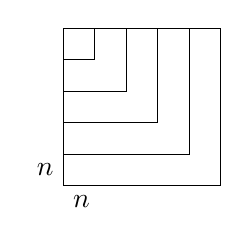
\begin{tikzpicture}
                \draw (0,0) -- (2,0) -- (2,2) -- (0,2) -- (0,0);
                \draw (0,0.4) -- (1.6,0.4) -- (1.6,2) -- (0,2) -- (0,0);
                \draw (0,0.8) -- (1.2,0.8) -- (1.2,2) -- (0,2) -- (0,0); 
                \draw (0,1.2) -- (0.8,1.2) -- (0.8,2) -- (0,2) -- (0,0) node[above left]{$n$};
                \draw (0,1.6) -- (0.4,1.6) -- (0.4,2) -- (0,2) -- (0,0) node[below right]{$n$};
            \end{tikzpicture}
        \end{center}

        This means that the determinant of the matrix obtained by taking the first $k$ rows and columns of $S$ is positive, $\forall k = 1, \dots, n$.
    \end{multicols}

    \item Cholesky decomposition: $S = B^\intercal B$, with $B$ upper triangular
    \item All pivot elements are positive in the Gaussian elimination process
\end{enumerate}

Let's consider $\lambda > 0$ being a certain eigenvalue. 
\[ 
    S\underline{x} = \lambda\underline{x}    
\]
We multiply both sides by $\underline{x}^\intercal$:
\[
    \underline{x}^\intercal S\underline{x} = \lambda\underline{x}^\intercal\underline{x} = \lambda\||\underline{x}\||^2 \geq 0
\]
Recall that $\underline{x}$ is an eigenvector while the before considered vector $\underline{v}$ is a generic vector. With $\underline{v}$, instead, we have:
\[
    \underline{v} = (c_1\underline{x}_1 + c_2\underline{x}_2 + \dots + c_n\underline{x}_n)    
\]
So we are expressing $\underline{v}$ as a linear combination of the eigenvectors of $S$. 
\[
    (c_1\underline{x}_1 + c_2\underline{x}_2 + \dots + c_n\underline{x}_n)^\intercal S (c_1\underline{x}_1 + c_2\underline{x}_2 + \dots + c_n\underline{x}_n)        
\]
\[
    \begin{rcases}
        c_1^2\underline{x}_1^\intercal S \underline{x}_1 = c_1^2\lambda_1\underline{x}_1^\intercal \underline{x}_1 = c_1^2\lambda_1||\underline{x}_1||^2\\
        c_1c_2\underline{x}_1^\intercal S \underline{x}_2 = c_1c_2\lambda_2\underline{x}_1^\intercal \underline{x}_2 = 0\\
    \end{rcases}    
    \text{there are two types of components}
\]
The first components is given by the eigenvectors with the same direction, while the second no so their scalar product is null (they are orthogonal).\\

From \textit{iv}):
\[
    S = B^\intercal B \implies \underline{v}^\intercal(B^\intercal B)\underline{v} = (\underline{v}^\intercal B^\intercal)(B \underline{v}) = (B\underline{v})^\intercal (B\underline{v}) = ||B\underline{v}||^2 \geq 0   
\]

\section{Singular Value Decomposition (SVD)}
We are going to use it for:
\begin{itemize}
    \item Least-squares approximation by introducing the pseudo-inverse of a matrix (Moore-Penrose inverse)
    \item Low-rank approximation with the Eckart-Young theorem
\end{itemize}
We start from:
\[
A \in \mathbb{R}^{m \times n} \hspace{1cm} 
\begin{cases}
m = \text{\# of samples}\\
n = \text{\# of features}
\end{cases}    
\]
We can write:
\[
    A = U\Sigma V^\intercal    
\]
With:
\begin{itemize}
    \item $U$ with dimensions $m \times m$ and orthogonal
    \item $\Sigma$ with dimensions $m \times n$ \textit{almost} diagonal
    \item $V^\intercal$ with dimensions $n \times n$ and orthogonal
\end{itemize}
If $m > n$, we can represent the matrices like this:
\[
\underbrace{
  \begin{bmatrix}
    & & & & & \\
    & & & & & \\
    & & & & & \\
    & & & & & \\
    & & & & & \\
  \end{bmatrix}}_{m \times m}
\underbrace{
  \begin{bmatrix}
    & & & \\
    & & & \\
    & & & \\
    & & & \\
    & & & \\
  \end{bmatrix}}_{m \times n}
\underbrace{
  \begin{bmatrix}
    & & & \\
    & & & \\
    & & & \\
  \end{bmatrix}}_{n \times n}
\]
What is the idea of SVD? Try to change features so variances are maximized and covariances are minimized. We don't want columns to be correlated.\\

In general: rank($A$) = $r < n$.
\[
    AV = U\Sigma \impliedby V^\intercal V = I \impliedby V \text{ is orthogonal}    
\]
The component wise notation is:
\[
    A\underline{v_i} = \sigma_i\underline{u_i}    
\]
Given that the rank of $A$ is $r$:

\[
\begin{bmatrix}
    & & & & & & &\\
    & & & & & & &\\
    & & & & & & &\\
    & & & & & & &\\
    & & & & & & &\\
    & & & & & & &\\
\end{bmatrix}
\begin{bmatrix}
    \sigma_1 & & & &\\
    & \sigma_2 & & &\\
    & & \ddots & &\\
    & & & \sigma_r &\\
    & & & & 0\\
    \hline
    0 & 0 & 0 & 0 & 0\\
    0 & 0 & 0 & 0 & 0\\
\end{bmatrix}
\begin{bmatrix}
    & & & & \\
    & & & & \\
    & & & & \\
    & & & & \\
\end{bmatrix}
\hspace{1cm}
\begin{cases}
\sigma_1, \dots, \sigma_r > 0\\
\sigma_{r+1}, \dots, \sigma_n = 0
\end{cases}  
\]
Typically: $\sigma_1 > \sigma_2 > \dots > \sigma_r > \sigma_{r+1} = 0$.
We have:
\[
\begin{cases}
    \begin{rcases}
        A\underline{v_1} = \sigma_1\underline{u_1}\\
        \hspace{1cm}\vdots\\
        A\underline{v_r} = \sigma_r\underline{u_r}\\        
    \end{rcases} r\\
    \begin{rcases}
        A\underline{v_{r+1}} = \sigma_{r+1}\underline{u_{r+1}}\\
        \hspace{1cm}\vdots\\
        A\underline{v_n} = \sigma_n\underline{u_n}\\        
    \end{rcases} n-r
\end{cases}    
\]
So the first $r$ vectors span the column space of $A$ while for the last $n-r$ means that $\underline{v_i} \in N(A)$ for $i = r+1, \dots, n$.
If we have $A^\intercal$, the decomposition is $A^\intercal = (U\Sigma V^\intercal)^\intercal = V\Sigma^\intercal U^\intercal$. 

\subsection{Economy SVD}
What we've seen so far is the full SVD, but it can be optimized. Here is following the compact (reduced) representation, where once again we consider $m > n$:
\[
\underbrace{
  \begin{bmatrix}
    & & & \\
    & & & \\
    & & & \\
    & & & \\
    & & & \\
  \end{bmatrix}}_{m \times n}
\underbrace{
  \begin{bmatrix}
    & & & \\
    & & & \\
    & & & \\
  \end{bmatrix}}_{n \times n}
\underbrace{
  \begin{bmatrix}
    & & & \\
    & & & \\
    & & & \\
  \end{bmatrix}}_{n \times n}
\]
This is caused by the fact that the last $m-n$ rows in the central matrix are all 0 so multiply them for the last $m-n$ columns of the left matrix is useless. This can be furthermore optimized by having matrix dimensions: $(m\times r)(r\times r)(r\times n)$ because not all $\sigma$ might be different than 0 (i.e. the rank of $A$ is $r$), so, in that case is useless even to multiply the last $m-r$ rows of the central matrix. \\

\textbf{The SVD works for any matrix $A$.}\\

\noindent Let's suppose $A$ is full rank $n\times n$:
\[
    A = U\Sigma V^\intercal = \sum_{i = 1}^{n} \sigma_i \underbrace{\underline{u_i}\underline{v_i}^\intercal}_{\text{rank }=1}    
\]
View matrix-matrix multiplication for the rank 1 concept.
If $A$ is not full rank but instead has rank($A$)=$r$, the same sum is nomore computed until $n$, but instead $r$.
\[
    A = \sum_{i = 1}^{r} \sigma_i \underline{u_i}\underline{v_i}^\intercal   
\]
What happens now if we pick a certain value $\tilde{r} < r$?
\[
    A = U\Sigma V^\intercal \cong \sum_{i = 1}^{\tilde{r}} \sigma_i \underline{u_i}\underline{v_i}^\intercal   
\]
We obtain a \textbf{rank $\tilde{r}$ approximation of the matrix A}. The rank of the matrix is know because is the sum of $\tilde{r}$ matrices of rank 1. Moreover, that one, is the best approximation of rank $\tilde{r}$ possible, i.e.:
\[
    ||A - \tilde{A}|| \leq ||A - B|| \hspace{1cm} \forall B  \text{ of rank} = \tilde{r}    
\]

\subsection{Proof of the existence of SVD}
Once again, we start from matrix $A \in \mathbb{m \times n}$ an rank$=r$. We consider the new matrix $A^\intercal A$ which is:
\begin{itemize}
    \item symmetric: $(A^\intercal A)^\intercal = A^\intercal A$
    \item positive definite: $\underline{x}^\intercal(A^\intercal A)\underline{x} = (\underline{x}^\intercal A^\intercal)(A \underline{x}) = (A\underline{x})^\intercal (A\underline{x}) = ||A\underline{x}||^2 \geq 0  $
\end{itemize} 
We can use the following decomposition:
\[
    A^\intercal A = V\Lambda V^\intercal = \sum_{i=1}^n \lambda_i \underline{v_i} \underline{v_i^\intercal}    
\]
Recall that $V$ contains the eigenvectors while $\Lambda$ contains the eigenvalues. We rename $\lambda_i = \sigma_i^2$. The rank of $A^\intercal A$ is $r$.\\

We want to prove that if  $\underline{x} \in N(A)$ then $\underline{x} \in N(A^\intercal A)$, to do so we proceed in both directions:
\begin{enumerate}
    \item If we have $A\underline{x} = 0 \implies \underline{x} \in N(A)$. Is it possible to multiply both terms:
    \[
        A^\intercal(A\underline{x}) = A^\intercal \underline{0} = \underline{0} \hspace{1cm} \text{so} \hspace{1cm} \underline{x} \in N(A) \implies \underline{x} \in N(A^\intercal A)
    \]
    \item We start from $(A^\intercal A)\underline{x} = 0 \implies \underline{x} \in N(A^\intercal A)$. Again, we multiply:
    \[
        \underline{x}^\intercal A^\intercal A\underline{x} = ||A\underline{x}||^2 = 0 \hspace{1cm} \text{so} \hspace{1cm} \underline{x} \in N(A^\intercal A) \implies \underline{x} \in N(A)
    \]
\end{enumerate}
Let's consider the couple of (eigenvalues, eigenvectors) = ($\sigma_i^2, \underline{v_i}$):
\[
    A^\intercal A\underline{v_i} = \sigma_i^2 \underline{v_i} \hspace{0.3cm}\overset{\text{component-wise}}{\longrightarrow} \hspace{0.3cm} A^\intercal A\underline{v_i} = \sigma_i^2 \underline{v_i} \hspace{1cm} (\dagger)
\]
We introduce the quantity $\underline{u_i} = \dfrac{A\underline{v_i}}{\sigma_i}$ which has some characteristics:
\begin{enumerate}[i]
    \item $\underline{u_i}$ are unitary vectors:
    \[
        \underline{u_i}^\intercal \underline{u_i} = \left(\dfrac{A\underline{v_i}}{\sigma_i}\right)^\intercal \left(\dfrac{A\underline{v_i}}{\sigma_i}\right) = \dfrac{\underline{v_i^\intercal}A^\intercal A\underline{v_i}}{\sigma^2} \overset{\dagger}{=} \dfrac{\sigma_i^2 \underline{v_i^\intercal}\underline{v_i}}{\sigma_i^2} = 1
    \]
    The last passage of the equation is true because $\underline{v_i}$ vectors are orthonormal.
    \item $\underline{u_i} \perp \underline{u_j}$:
    \[
        \underline{u_i}^\intercal \underline{u_j} = \left(\dfrac{A\underline{v_i}}{\sigma_i}\right)^\intercal \left(\dfrac{A\underline{v_j}}{\sigma_j}\right) = \dfrac{\underline{v_i^\intercal}A^\intercal A\underline{v_j}}{\sigma_i \sigma_j} \overset{\dagger}{=} \dfrac{\sigma_j^2 \underline{v_i^\intercal}\underline{v_j}}{\sigma_i \sigma_j} = 0
    \] 
    \item $\underline{u_i}$ are eigenvectors of $AA^\intercal$ with eigenvalues $\sigma_i^2$:
    \[
        (AA^\intercal \underline{u_i}) = AA^\intercal\left(\dfrac{A\underline{v_i}}{\sigma_i}\right) = A\dfrac{A^\intercal A\underline{v_i}}{\sigma_i} \overset{\dagger}{=} A\dfrac{\sigma_i^2 \underline{v_i}}{\sigma_i} = \sigma_i^2\left(\dfrac{A\underline{v_i}}{\sigma_i}\right) = \sigma_i^2\underline{u_i}   
    \]
\end{enumerate}
We have demonstrated that $A\underline{u_i} = \sigma_i \underline{u_i}$ and $\underline{u_i}$ are orthonormal as well. 
We have seen that $\underline{u_i} = \frac{A\underline{v_i}}{\sigma_i}$ but, what happen if $\sigma_i = 0$?\\
Until now we have assumed that could not happen. Let's 2 examples, in the first we have the standard case while in the second is explained how to manage the case $\sigma_i = 0$.\\

\textbf{Example 1}
\[
A = \begin{bmatrix}
    4 & 4\\
    -3 & 3\\
\end{bmatrix} \hspace{1cm} \text{rank}(A) = 2
\]
We build two new matrices $X$ and $Y$:
\[
X = A^\intercal A = \begin{bmatrix}
    25 & 7\\
    7 & 25\\
\end{bmatrix} \hspace{1cm} \text{eigs}(X) = 
\begin{cases}
    \lambda_1 = 18 \hspace{1cm} \underline{v_1} = \begin{bmatrix}
        -\frac{\sqrt{2}}{2}\\
        \frac{\sqrt{2}}{2}\\
    \end{bmatrix}\\
    \lambda_2 = 32 \hspace{1cm} \underline{v_2} = \begin{bmatrix}
        \frac{\sqrt{2}}{2}\\
        \frac{\sqrt{2}}{2}\\
    \end{bmatrix}\\
\end{cases}    
\]
\[
Y = AA^\intercal = \begin{bmatrix}
    32 & 0\\
    0 & 18\\
\end{bmatrix} \hspace{1cm} \text{eigs}(Y) =
\begin{cases}
    \lambda_1 = 18 \hspace{1cm} \underline{u_1} = \begin{bmatrix}
        1\\
        0\\
    \end{bmatrix}\\
    \lambda_2 = 32 \hspace{1cm} \underline{u_2} = \begin{bmatrix}
        0\\
        1\\
    \end{bmatrix}\\
\end{cases}    
\]
So we have all elements for contructing the SVD:
\[
U = 
\begin{bmatrix}
    0 & 1\\
    1 & 0\\
\end{bmatrix}
\hspace{1cm}
\Sigma =
\begin{bmatrix}
    \sqrt{18} & 0\\
    0 & \sqrt{32}\\
\end{bmatrix}    
\hspace{1cm}
V =
\begin{bmatrix}
    -\frac{\sqrt{2}}{2} & \frac{\sqrt{2}}{2}\\
    \frac{\sqrt{2}}{2} & \frac{\sqrt{2}}{2}\\
\end{bmatrix}
\]
It is easy to verify that $A = U\Sigma V^\intercal$.

\textbf{Example 2}
\[
A = \begin{bmatrix}
    4 & 3\\
    8 & 6\\
\end{bmatrix}
\hspace{1cm}
\text{rank}(A) = 1    
\]\\
As in the example before, we start building our matrices $X$ and $Y$:
\[
X = A^\intercal A = \begin{bmatrix}
    80 & 60\\
    60 & 45\\
\end{bmatrix}
\hspace{1cm}
\text{eigs}(X) =
\begin{cases}
    \lambda_1 = 125 \hspace{1cm} \underline{v_1} = \begin{bmatrix}
        \frac{-4}{5}\\
        \frac{-3}{5}\\
    \end{bmatrix}\\
    \lambda_2 = 0 \hspace{1cm} \underline{v_2} = ?
\end{cases}
\]
How can we compute the value of $\underline{v_2}$? The idea is to bild a vector $\underline{v_2}$ such that it is orthogonal to $\underline{v_1}$. 
A possible solution is: $\underline{v_2} = \begin{bmatrix}
    \frac{3}{5}\\
    \frac{-4}{5}\\
\end{bmatrix}$.\\
The equation at the beginning of this page (the one regarding $\underline{u_i}$) can still be computed for the vector $\underline{v_1}$ in this case:
\[
\underline{u_1} = \dfrac{A\underline{v_1}}{\sigma_1} = \dfrac{1}{\sqrt{125}}\begin{bmatrix}
    4 & 3\\
    8 & 6\\
\end{bmatrix}
\begin{bmatrix}
    \frac{-4}{5}\\
    \frac{-3}{5}\\
\end{bmatrix} = \dfrac{1}{\sqrt{125}}\begin{bmatrix}
-5\\
-10\\    
\end{bmatrix}
\]
Now, the problem rises again because $\sigma_2 = 0$ so we cannot compute $\underline{u_2}$. In reality, we do not need to compute $\underline{u_2}$ because $\underline{u_1}$ and $\underline{v_1}$ are sufficient to recover the original matrix through (reduced) SVD, indeed:
\[
\underbrace{
\dfrac{1}{\sqrt{125}} \begin{bmatrix}
    -5 \\
    -10\\
\end{bmatrix}}_{U}
\underbrace{
\begin{bmatrix}
    \sqrt{125}
\end{bmatrix}}_{\Sigma}
\underbrace{ 
\begin{bmatrix}
    \frac{-4}{5} & \frac{-3}{5}\\
\end{bmatrix}}_{V}   
=
\begin{bmatrix}
    4 & 3\\
    8 & 6\\
\end{bmatrix}
\] 
We could have used also the full SVD with the following matrices:
\[
    U = \dfrac{1}{\sqrt{125}} \begin{bmatrix}
        -5 & -10\\
        -10 & 5\\
    \end{bmatrix}
\hspace{1cm}
\Sigma = \begin{bmatrix}
    \sqrt{125} & 0\\
    0 & 0\\
\end{bmatrix}
\hspace{1cm}
V = \begin{bmatrix}
    \frac{-4}{5} & \frac{-3}{5}\\
    \frac{-3}{5} & \frac{4}{5}\\
\end{bmatrix}
\]
Where $\underline{u_2}$ is the second column of the matrix $U$ and is a vector orthogonal to $\underline{u_1}$. All elements written here and not in the previous formulation are a waste of memory.
A concise recap of all versions of SVD:
\begin{enumerate}
    \item \textbf{full SVD}: $\underset{(m \times n)}{A} = \underset{(m \times m)}{U}\underset{(m \times n)}{\Sigma}\underset{(n \times n)}{V^\intercal}$
    \item \textbf{economy SVD}: $\underset{(m \times n)}{A} = \underset {(m \times n)}{U}\underset{(n \times n)}{\Sigma}\underset{(n \times n)}{V^\intercal}$
    \item \textbf{reduced SVD}: $\underset{(m \times n)}{A} = \underset{(m \times r)}{U}\underset{(r \times r)}{\Sigma}\underset{(r \times n)}{V^\intercal}$
    \item \textbf{truncated SVD approximation}: $\sum\limits_{i=1}^{\tilde{r}} \sigma_i\underline{u_i}\underline{v_i^\intercal}$
\end{enumerate}
For the first two cases the rank of $A$ is $n$, for the third is $r$ while in the first the approximation rank is decided.

\subsection{Geometrical interpretation of SVD}
Matrices $U, V^\intercal$ are orthonormal so, as mentioned in the section above, they represent a rotation (or reflection) while $\Sigma$, being a diagonal matrix, correspond to a scaling transformation. 
\begin{center}
    \includegraphics[scale=0.4]{../images/SVD_Geometric_Interpretation.png}
\end{center}
\textbf{Since for SVD no assumptions are made on the starting matrix, this means that \underline{any} matrix can be obtained from 2 rotations and 1 scaling.}\\

When $A$ is squared and symmetric ($A \in \mathbb{R}^{n\times n}, A=A^\intercal$)?

We can apply \textbf{polar decomposition}:
\[
A = QR    
\]
Where $Q$ is orthogonal and $S$ is symmetric positive semi-definite. Why? From SVD. 
\[
    A = U\Sigma V^\intercal = \underbrace{(UV^\intercal)}_{Q}\underbrace{(V\Sigma V^\intercal)}_{S}    
\]
In particular, the product of the two orthogonal matrices in the first parenthesis is always another orthogonal matrix. In this case of decomposition, matrix $A$ is obtained just by one rotation and one scaling (missing one more rotation with respect to classic SVD). Indeed, the second parenthesis results just in a stretch because $V$ and $V^intercal$ are two rotations identical and opposite, i.e. they cancels out. 

\subsubsection{Properties of SVD}
\begin{enumerate}[i]
    \item If A is orthogonal, then $\sigma_i = 1$ because if $A$ orthogonal then $A^\intercal A = I$
    \item All eigenvalues of a square matrix are $\leq \sigma_1$. Proof:
    \[
        ||A\underline{x}|| = ||U\Sigma V^\intercal \underline{x}|| = ||\Sigma V^\intercal \underline{x}|| \leq \sigma_1||V^\intercal \underline{x}|| = \sigma_1||\underline{x}|| \implies ||A\underline{x_i}|| \leq \sigma_1||\underline{x_i}||
    \]
    The matrix $U$ disappear becuase an orthogonal matrix, when multiplied, does not change the magnitude of a vector. If we consider
    \[
        ||A\underline{x_i}|| = ||\lambda_i\underline{x_i}|| = |\lambda_i|\cdot ||\underline{x_i}||
    \]
    \[
        |\lambda_i|\cdot ||\underline{x_i}|| \leq \sigma_1||\underline{x_i}|| \implies |\lambda_i| \leq \sigma_1 \hspace*{0.4cm} \forall i    
    \]
\end{enumerate}

\subsection{Snapshots method}
During real case scenarios, we will have a certain matrix $A \in \mathbb{m\times n}$ and it might happen that $m \gg n$ i.e. the number of samples is much greater than the number of features. In these cases, we can use the following trick to be more efficient.

For the SVD we need to compute both $AA^\intercal$ and $A^\intercal A$. Which one is better to start with? And why?
We would have $AA^\intercal: (m\times m)$ and $A^\intercal A: (n\times n)$. Given $m \gg n$ it is clear that the second one is better to start with becuase, being much smaller, it will be easier to computer its eigenvalues and eigenvectors.    


\subsection{Matrix norms}
This concept is an extension of the vector norm. Given a matrix $A \in \mathbb{R}^{m\times n}$, we define the matrix norm as:
\begin{itemize}
    \item \textbf{Frobenius norm}: $||A||_F = \sqrt{\sum\limits_{i=1}^{m}\sum\limits_{j=1}^{n}|a_{ij}|^2} = \sqrt{\Tr(A^\intercal A)} = \sqrt{\Tr(AA^\intercal)}$ \\
    Recall that $\Tr(AB) = \Tr(BA)$. \\
    Example:
    \[
        A = \begin{bmatrix}
            1 & 2\\
            3 & 4\\
            5 & 6\\
        \end{bmatrix} \hspace{1cm} ||A||_F = \sqrt{1^2 + 2^2 + 3^2 + 4^2 + 5^2 + 6^2} = \sqrt{91}
    \]
    \[
        \begin{bmatrix}
            1 & 2\\
            3 & 4\\
            5 & 6\\
        \end{bmatrix}
        \begin{bmatrix}
            1 & 3 & 5\\
            2 & 4 & 6\\
        \end{bmatrix} =
        \begin{bmatrix}
            1^2+2^2 & \hdots & \hdots\\
            \hdots & 3^2+4^2 & \hdots\\
            \hdots & \hdots & 5^2+6^2\\
        \end{bmatrix}  \implies \sqrt{\Tr(AA^\intercal)} = \sqrt{91}    
    \]
    If $U$ is orthogonal, what happen to $||AU||^2_F$?
    \[
        ||AU||^2_F = \Tr((AU)^\intercal AU) = \Tr(U^\intercal A^\intercal AU) = \Tr(A^\intercal A\underbrace{UU^\intercal}_{I}) = \Tr(A^\intercal A) = ||A||^2_F    
    \]
    This means that the Frobenius norm is invariant with respect to orthogonal transformations ($\dag$). \\ 
    The Frobenius norm is also equal to $\left(\sqrt{\sum\limits_{i=1}^{r}\sigma_i^2}\right)$ where $r$ is the rank of $A$. Proof:
    \[
        ||A||_F = ||U\Sigma V^\intercal||_F \overset{\dag}{=} ||\Sigma||_F \triangleq  \Tr\sqrt{(\Sigma\Sigma^\intercal)} = \sqrt{\sum\limits_{i=1}^{r}\sigma_i^2}    
    \]
    \item \textbf{P-norms}: Recall the p-norm for vectors:
    \[
        \underline{p} \in \mathbb{R}^n \implies ||\underline{p}||_p = \left(\sum\limits_{i=1}^n |p_i|^p\right)^{\frac{1}{p}}    
    \]
    Given $A \in \mathbb{R}^{m\times n}$ we can define the p-norm for that matrix as:
    \[
        ||A||_p = \underset{\underline{x} \in \mathbb{R}^n}{\sup} \dfrac{||A\underline{x}||_p}{||\underline{x}||_p} = \underset{\underline{x} \in \mathbb{R}^n, \hspace{0.1cm} ||\underline{x}||_p}{\sup} ||A\underline{x}||_p
    \]
    If you choose $p=2$ you get the operator norm and $||A||_2 = \sigma_1$.
\end{itemize}

\subsection{Eckart-Young theorem}
Having defined the norms, we can now proceed with the proof of the \textbf{Eckart-Young theorem} which states:\\

\emph{For either $||\cdot||_F$, $||\cdot||_2$ we have:}
\[
    ||A - A_k|| \leq ||A - B|| \hspace{1cm} \forall B \text{ of rank } k
\]
\emph{where} $A_k = \sum\limits_{i=1}^k \sigma_i\underline{u_i}\underline{v_i}^\intercal$ \emph{i.e. is the SVD approximation of rank k of the matrix A. Depending on the chosen norm you get:}
\[
    ||A - A_k|| = \begin{cases}
        \sigma_{k+1} \text{ if } ||\cdot||_2 \text{considered}\\
        \left(\sum\limits_{i=1}^{r} \sigma_i^2\right)^{\frac{1}{2}} \text{ if } ||\cdot||_F \text{ considered}
    \end{cases}
\]
There will be 2 proofs, one for each type of norm. 

\subsubsection{Proof considering $||\cdot||_F$}
We start from the \textbf{Weyl inequality}:
\[
    \sigma_{i+j-1}(X+Y) = \sigma_i(X) + \sigma_j(Y)    
\]
Where a generic $\sigma_k(E)$ is the k-eiths singular value of the matrix $E$.  
We define 
\[
X = A_k - B \hspace{2cm} Y = B    
\]
So we have
\[
\sigma_{i+k}(A) \leq \sigma_i(A-B) + \underbrace{\sigma_{k+1}(B)}_{0}
\]
The last component has value of 0 because the matrix $B$ has rank equal to $k$.
\[
||A - A_k||_F^2 = \left(\sum\limits_{i=k+1}^r \sigma_i^2(A)\right) \overset{\text{shift}}{\overset{\downarrow}{=}} \left(\sum\limits_{i=1}^{r-k} \sigma_{i+k}^2(A)\right) \leq \left(\sum\limits_{i=1}^{r-k} \sigma_{i+k}^2(A - B)\right) \leq \left(\sum\limits_{i=1}^{\min(m,n)} \sigma_{i+k}^2(A-B)\right) = ||A-B||_F^2
\]
In particular, recall that $A = \sum\limits_{i=1}^{r} \sigma_i\underline{u_i}\underline{v_i^\intercal}$ and $A_k = \sum\limits_{i=1}^{k} \sigma_i\underline{u_i}\underline{v_i^\intercal}$. The theorem is proved just by picking the first and last components of the inequality written above. 



\subsubsection{Proof considering $||\cdot||_2$}
We are now going to prove the theorem with the last norm we did not use yet. Let's consider the matrix $B$ with dimensions $n \times d$ and rank($B$)=$k$. This means that:
\[
    N(B) \subset \mathbb{R}^d \hspace{1cm} dim(N(B)) = d-k     
\]
If we consider matrix $V$ of the SVD decomposition of $A$:
\[
    V_{k+1} = \underbrace{\begin{bmatrix}
        \vline & \vline & \vline\\
        \underline{v_1} & \ldots & \underline{v_{k+1}}\\
        \vline & \vline & \vline
    \end{bmatrix}}_{k+1 \text{cols}}
\]
Those are the $k+1$ columns of $V$.
\[
\mathcal{C}(V_{k+1}) \subset \mathbb{R}^d  \hspace{1cm} dim(\mathcal{C}(V_{k+1})) = k+1  
\]
By adding the previous information, we have:
\[
    dim(N(B)) + dim(\mathcal{C}(V_{k+1})) = d - k + k + 1 = d + 1 
\]
Since both spaces are subset of $\mathbb{R}^d$ and their summed dimensions are $d+1$ this means that the intersection of those spaces is not empty.\\ 
\begin{center}
    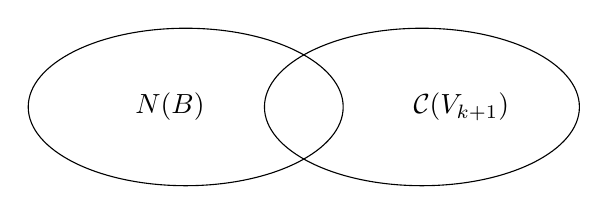
\begin{tikzpicture}
        \draw (0,0) ellipse (2cm and 1cm);
        \draw node at (-0.2,0) {$N(B)$};
        \draw (3,0) ellipse (2cm and 1cm);
        \draw node at (3.5,0) {$\mathcal{C}(V_{k+1})$};
    \end{tikzpicture}
\end{center}
Consider $\underline{w} \in N(B) \bigcap \mathcal{C}(V_{k+1})$, we suppose for easyness that $||\underline{w}||_2 = 1$.
\[
    \underline{w} = \sum_{i=1}^{k+1} c_i \underline{v_i} \overset{(\star)}{=} V_{k+1}\underline{c} \hspace{1cm} \sum_{i=1}^{k+1} c_i^2 = 1   
\]
We want to measure the following quantity:
\[
    ||A - B||^2_2 =  \underbrace{\underset{||\underline{w}||}{\sup} ||(A-B)\underline{w}||_2^2}_{\text{particular $||\underline{w}||$}} \geq \underbrace{||(A-B)\underline{w}||_2^2}_{\text{generic $||\underline{w}||$}} \implies
\]
Recall that $\underline{w} \in N(B) \implies B\underline{w} = 0$.
\[
    \implies ||A-B||^2_2 \geq ||A\underline{w}||_2^2 = \underline{w}^\intercal A^\intercal A \underline{w} \overset{\text{SVD}}{=} \underline{w}V\Sigma^\intercal \underbrace{U^\intercal U}_{I} \Sigma V^\intercal  \underline{w} = 
\] 
\[
    ? \underline{w}^\intercal V\Sigma^\intercal \Sigma V^\intercal \underline{w} \overset{(\star)}{=} \underline{c}^\intercal \underbrace{V_{k+1}^\intercal V_{k+1}}_{I} \Sigma^\intercal \Sigma  \underbrace{V_{k+1}^\intercal V_{k+1}}_{I} \underline{c} = \underline{c}^\intercal \Sigma^\intercal \Sigma \underline{c} = \sum_{i=1}^{k+1} c_i^2 \sigma_i^2 \geq    
\] 
Since singular values are ordered
\[
    \geq \sigma_{k+1}^2 \underbrace{\sum_{i=1}^{k+1} c_i^2} = \sigma_{k+1}^2    
\]
So
\[
    ||A-B||_2^2 \geq \sigma_{k+1}^2 = ||A - A_k||_2^2    
\]
And, erasing the squares:
\[
    ||A - B||_2^2 \geq \sigma_{k+1} = ||A - A_k||_2        
\]
Where $A_k$ is the rank $k$ truncated SVD approximation, therefore
\[
    ||A - A_k||_2 \leq ||A - B||_2 \hspace{1cm} \forall B \text{ of rank } k
\]


\section{PCA}
Here is a first real-world application of the SVD. PCA has the same aim as SVD i.e. find a way of projecting the dataset in a new space where variances are maximized and covariances are minimized. 

We start from $A \in \mathbb{R}^{n \times d}$ and we follow these points:
\begin{enumerate}[i]
    \item \textbf{Center the matrix \emph{A}}\\
    $\bar{A}$ is the mean centered with respect to columns while $H$ is called the centering matrix and is obtained as follows:
    \[
        H = I_n - \dfrac{1}{n} \underline{\mathbbm{1}}_n \underline{\mathbbm{1}}_n^\intercal
    \]
    Where $\underline{\mathbbm{1}}_n$ is the vector of dimension $n$ containing all ones. The centered matrix is obtained:
    \[
        \bar{A} = HA    
    \]
    \item Build the covariance matrix
    \[
        S = \dfrac{\bar{A}^\intercal \bar{A}}{n - 1}     
    \]
    Where the denominator is $n-1$ is because we want an unbiased estimator and it's not $n$ because we have already taken 1 degree of freedom by centering the matrix. The covariance matrix is semidefinite positive so we can use eigenvalues and eigenvectors decomposition.
    \[
        SV = VD \implies VDV^\intercal, D = V^\intercal SV    
    \]
    If you order the eigenvalues in decreasing order the corresponding eigenvectors are called principal components. To notice the relationship between SVD and PCA we can write:
    \[
        S = \dfrac{1}{n-1}\bar{A}^\intercal \bar{A} = \dfrac{1}{n-1} V\Sigma^\intercal U^\intercal U \Sigma V^\intercal = \dfrac{1}{n-1} V \Sigma^2 V^\intercal    
    \]
    \[
        D = \dfrac{1}{n-1}\Sigma^2 \implies \lambda_k \dfrac{\sigma_k^2}{n-1}    
    \]
\end{enumerate}
PCA is SVD applied to a particular matrix.


\subsection{Choose rank of truncated SVD}
When using truncated SVD, how to choose the rank $k$? One possibility is to use $k$ such that a predefined percentage of the variance is retained. Another idea starts from:
\[
    A = A_{true} + \gamma A_{noise}    
\]
Where: 
\begin{itemize}
    \item $A$: is out dataset
    \item $A_{true}$: is the underlying low-rank representation of our data
    \item $\gamma$: magnitude of the noise
    \item $A_{noise}$: is a gaussian noise with 0 mean and unitary variance
\end{itemize}
By defining $\tau$ as threshold we have that if $sigma_i > \tau$ we are picking $A_{true}$. 
There are two cases:
\begin{itemize}
    \item $\gamma$ is known, i.e. we know the magnitude of the noise:
    \begin{itemize}
        \item if $A \in \mathbb{R}^{n \times n}$ (square) then $\tau = \dfrac{4}{\sqrt{3}}\gamma \sqrt{n}$
        \item if $A \in \mathbb{R}^{m \times n}$ we have two more cases:
        \begin{itemize}
            \item if $n \ll m \implies \tau = \lambda(\beta)$ where $\beta = \dfrac{n}{m}$ and $\lambda$ is the following function:
            \[
                \lambda(\beta) = \sqrt{2(\beta + 1) + \dfrac{8\beta}{(\beta+1)+\sqrt{(\beta^2 + 14\beta + 1))}}}    
            \]
            \item if $m \ll n \implies \tau = \lambda(\beta)$ where $\beta = \dfrac{m}{n}$ so it's equal as before but in this case the numerator and denumerator of $\beta$ are swapped.
        \end{itemize}
    \end{itemize}
    \item $\gamma$ is unknown. We define $\tau$ as follows:
    \[
        \tau = \omega(\beta)\sigma_{med} \hspace{1cm} \omega(\beta) = \dfrac{\lambda(\beta)}{\mu_{\beta}}    
    \]
    In which $\sigma_{med}$ is the median of the singular values and $\mu_{\beta}$ is the median of the Marcenko-Pastur distribution. $\lambda(\beta)$ is the same function as before. In particular:
    \[
        \mu_{\beta} = \int_{(1-\beta)^2}^{\mu_{\beta}} \dfrac{\sqrt{((1- \sqrt{\beta})^2 - t)(t - (1- \sqrt{\beta})^2)}}{2\pi t} dt = \dfrac{1}{2}    
    \]
\end{itemize}


\subsection{Randomize SVD}
\begin{tikzpicture}
    \
\end{tikzpicture}
\section{Least squares approximation}
Consider, with $n > p$: 
\[
    X \in \mathbb{R}^{n \times p} \hspace{1cm} n = \text{\# samples}, \hspace{0.1cm} p = \text{\# features}, \text{ rank(}X\text{)} = p   
\]
\[
    \underline{y} \in \mathbb{R}^n \hspace{1cm} \text{labels of each sample}    
\]
We have:
\[
\underbrace{
\begin{bmatrix}
    \horzbar & \underline{x_1^\intercal} & \horzbar\\
    \horzbar & \underline{x_2^\intercal} & \horzbar\\    
     & \vdots & \\
    \horzbar & \underline{x_n^\intercal} & \horzbar
\end{bmatrix}}_{p}
\hspace{1cm}
\underbrace{x_j}: \text{j-th column of \emph{X}}
\]
If we provide a new sample $\tilde{\underline{x}} \rightarrow \tilde{y}$ we want to predict $\tilde{y}$, i.e. the label, using the information we have from the training set.\\
We can use a linear model:
\[
    \tilde{y} = \tilde{\underline{x}}^\intercal \underline{w} \hspace{1cm} \underline{w} \in \mathbb{R}^p
\]
Typically $\underline{y} \neq X\underline{w}$ so $\underline{y}$ won't be precisely obtained with that multiplication. We will have to the approximation: $\hat{\underline{y}} = X\underline{w}$. So we can say that $\hat{\underline{y}} \in \mathcal{C}(X)$ while in general $\underline{y} \notin \mathcal{C}(X)$.
The error of the prediction is given by:
\[
    r_i(\underline{w}) = \underline{y_i} - \underline{\hat{y_i}}    
\] 
We define the \textbf{residual vector} as $\underline{r}(\underline{w})$ and our goal is to minimize its l2-norm squared: $||\underline{r}(\underline{w})||^2_2$.\\

Mathematically we can describe the problem as finding: $\hat{\underline{w}} = \underset{\underline{w}}{\arg\min}||\underline{r}(\underline{w})||^2_2$. There are two approaches possible:
\begin{enumerate}
    \item Geometrical interpretation
    \item By means of optimization procedures
\end{enumerate}
\subsection{Geometrical interpretation}
\begin{center}
    \includegraphics[scale = 0.4]{../images/OLS_geometric_interpretation.png}
\end{center}
So, a brief description of the figure above:
\begin{itemize}
    \item the plane is the space of the predictions $\mathcal{C}(X)$ indeed it is spanned by the column vectors of $X$ 
    \item the vector $\underline{y}$ is the vector of the label to be predicted
    \item the vector $X\hat{\beta}$ in the figure is our prediction $\hat{\underline{y}}$ and correspond to the projection of $\underline{y}$ on the plane $\mathcal{C}(X)$
    \item $\epsilon$ is the residual vector $\underline{r}(\underline{w})$ and represent the error between the predicted value and the actual label
\end{itemize}
If we pick $\underline{\overline{y}} \in \mathcal{C}(X)$ different from $\hat{\underline{y}}$ and their respective residuals: $\underline{\overline{r}} = \underline{y} - \underline{\overline{y}}$ and $\underline{\hat{r}} = \underline{y} - \underline{\hat{y}}$ we have that:
\[
    ||\underline{\hat{r}}||_2 \leq ||\underline{\overline{r}}||_2
\]
Indeed, $\underline{\hat{r}}$ is the orthogonal projection of $\underline{y}$ on $\mathcal{C}(X)$ and the orthogonal projection is the closest point to the vector $\underline{y}$ in the subspace $\mathcal{C}(X)$.\\
Because of this, we can also say that:
\[
    \underline{x_j^\intercal}\underline{\hat{r}} = 0 \hspace{0.5cm} j = 1, \dots, p    
\]
in matrix form:
\[
    X^\intercal \underline{\hat{r}} = \underline{0}   \implies X^\intercal (\underline{y} - \underline{\hat{y}}) = \underline{0} \implies X^\intercal (\underline{y} - X\underline{\hat{w}}) = \underline{0} \implies X^\intercal \underline{y} = X^\intercal X \underline{\hat{w}}
\]
In general the rank of the matrix $X^\intercal X$ is the same as the rank of $X$ so if $X$ is full rank then also $X^\intercal X$ is full rank and this imply that is invertible and we can find $\hat{\underline{w}}$ like this:
\[
    \hat{\underline{w}} = (X^\intercal X)^{-1}X^\intercal \underline{y}
\]
If we are using this linear model for a binary classification we have to apply to the predicted value $\hat{\underline{y}}$ a sign function in order to have the output restrained to \{-1,1\}.\\

\subsection{Optimization}
Here we exploit mathematics for solving the initial problem:
\[
    \hat{\underline{w}} = \underset{\underline{w}}{\arg\min}||\underline{r}(\underline{w})||^2_2 = \underset{\underline{w}}{\arg\min}||\underline{y} - X\underline{w}||^2_2 = \underset{\underline{w}}{\arg\min}(\underline{y} - X\underline{w})^\intercal(\underline{y} - X\underline{w}) =     
\]
\[
    = \underset{\underline{w}}{\arg\min} \bigg[\underline{y}^\intercal \underline{y} - (X\underline{w})^\intercal \underline{y} - \underline{y}^\intercal (X\underline{w}) + (X\underline{w})^\intercal X\underline{w}  \bigg]= \underset{\underline{w}}{\arg\min} \underbrace{\bigg[\underline{y}^\intercal \underline{y} - 2\underline{y}^\intercal X\underline{w} + \underline{w}^\intercal X^\intercal X\underline{w}\bigg]}_{F(\underline{w})}
\]
$F(\underline{w})$ is a \textbf{quadratic functional}. $X$ is full rank, $X^\intercal X$ is positive definite so this means that the functional is strictly convex and has a unique minimum.
So we can compute the gradient and set it to zero:
\[
    \nabla_{\underline{w}}F(\underline{w}) = -2X^\intercal \underline{y} + 2X^\intercal X\underline{w} = \underline{0}
\]
\textbf{Example 1 - Derivation}
\[
    F(\underline{w}) = \underline{w}^\intercal \underline{c} = w_1 c_1 + w_2 c_2 + w_3 c_3 = \underline{c}\underline{w}^\intercal \hspace{1cm} \underline{w}, \underline{c} \in \mathbb{R}^3    
\]
The gradient is:
\[
    \nabla F = \begin{bmatrix}
        \dfrac{\partial F}{\partial w_1}\\
        \dfrac{\partial F}{\partial w_2}\\
        \dfrac{\partial F}{\partial w_3}
    \end{bmatrix} = \begin{bmatrix}
        c_1\\
        c_2\\
        c_3
    \end{bmatrix} = \underline{c}    
\]
\textbf{Example 2 - Derivation}
\[
    F(\underline{w}) = \underline{w}^\intercal A \underline{w} = \sum_{i=1}^n \sum_{j=1}^n w_j a_{ij} w_i \hspace{1cm} A \in \mathbb{R}^{n \times n}    
\]
\[
    \dfrac{\partial}{\partial w_k}(w_j a_{ij} w_i) = \begin{cases}
        a_{ij}w_i & k=j\neq i\\
        w_j a_{ij} & k=i\neq j\\
        0 & k\neq i , k\neq j\\
        2w_k a_{ij} & k=i=j
    \end{cases}    
\]


In the last lecture we have introduced the least squares method. In particular we have mentioned the linear model for which:
\[
    \hat{\underline{y}} = X\hat{\underline{w}} \hspace{1cm} X \in \mathbb{R}^{n \times p} \hspace{0.4cm} \underline{\hat{y}} \in \mathbb{R}^n \hspace{0.4cm} n \geq p \hspace{0.4cm} X \text{ full rank}
\]
We have obtained:
\[
    \underline{\hat{w}} = (X^\intercal X)^{-1} X^\intercal \underline{y} \implies \underline{\hat{y}} = \underbrace{X(X^\intercal X)^{-1} X^\intercal}_{P_x} \underline{y}     
\]
The matrix $P_x$ dimension is given by the product of: $(n\times p)(p\times p)(p \times n) = (n\times n)$ and has this properties:
\begin{itemize}
    \item $P_x = P_x^2$
    \item $P_x$ is a projection matrix
\end{itemize}

Let's consider $U$ an orthogonal ($U^\intercal U = I$) matrix that contains the basis for $\mathcal{C}(X)$ this means that $\mathcal{C}(X) = \mathcal{C}(U)$. We can write:
\[
    \underline{\hat{y}} = X\underline{\hat{w}} = U\underline{\tilde{w}}    
\]
So this basically means that the predicted value of $y$ still a projection on a plane but this time the plane is spanned by the columns of $U$ and not by the columns of $X$. By substituting last equation in the minimization method for least squares we have:
\[
    \underline{\tilde{w}} = \underset{\underline{w}}{\arg\min} ||\underline{y} - U\underline{w}||^2_2 \implies \underline{\hat{y}} = U\underline{\tilde{w}} = U(U^\intercal U)^{-1}U^\intercal \underline{y} = UU^\intercal \underline{y} 
\]
This formulation is possible because this time in the parenthesis we have an orthogonal matrix and this means that $(U^\intercal U)^{-1} = U^\intercal U = I$. In general $UU^\intercal \neq I$ because it might be rectangular (while $U^\intercal U$ is always square).\\

\textbf{Example of usage of U}
We start from $X$:
\[
    X= \begin{bmatrix}
        1& 1 \\
        1 & 3\\
        0 & 0
    \end{bmatrix}
    \hspace{1cm}
    \underline{x_1} = \begin{bmatrix}
        1\\
        1\\
        0   
    \end{bmatrix}
    \hspace{1cm}
    \underline{x_2} = \begin{bmatrix}
        1\\
        3\\
        0
    \end{bmatrix}
\]
How do we build the orthogonal matrix $U$? We can use the Gram-Schmidt procedure:
\[
    \underline{u_1} = \dfrac{\underline{x_1}}{||\underline{x_1}||} = \begin{bmatrix}
        \dfrac{1}{\sqrt{2}}\\
        \dfrac{1}{\sqrt{2}}\\
        0
    \end{bmatrix}    
\]
\[
    \underline{{x'}_2} = \underline{x_2} - (\underline{x_2}^\intercal \underline{u_1})\underline{u_1} = \underline{x_2} - (\underline{u_1^\intercal} \underline{u_1})\underline{x_2} \implies 
    \underline{u_2} = \dfrac{\underline{{x'}_2}}{||\underline{{x'}_2}||} 
    = \begin{bmatrix}
        -\dfrac{1}{\sqrt{2}}\\
        \dfrac{1}{\sqrt{2}}\\
        0
    \end{bmatrix}    
\]
So, the overall matrix $U$ is:
\[
    U = \begin{bmatrix}
        \dfrac{1}{\sqrt{2}} & \dfrac{1}{\sqrt{2}}\\
        -\dfrac{1}{\sqrt{2}} & \dfrac{1}{\sqrt{2}}\\
        0 & 0
    \end{bmatrix}    \hspace{1cm}
    U^\intercal U = I \text{ and } UU^\intercal \neq I
\]
A drawback of Gram Schmidt is that, depending on the order chosen for the columns of $X$, the matrix $U$ can be different. Moreover, the order of vector columns of $U$ is meaningless. \\

Now, we want to exploit the SVD for computing the orthogonal matrix $U$. We start from the SVD of $X$:
\[
    X = U\Sigma V^\intercal    
\]
So
\begin{multicols}{2}
    \[
    \begin{split}
        \underline{\hat{w}} &= (X^\intercal X)^{-1} X^\intercal y\\
        & = (V\Sigma^\intercal U^\intercal U\Sigma V^\intercal)^{-1} V\Sigma^\intercal U^\intercal \underline{y} \\
        & = (V\Sigma^\intercal \Sigma V^\intercal)^{-1} V\Sigma^\intercal U^\intercal \underline{y}\\
        & = V(V\Sigma^\intercal \Sigma V^\intercal)^{-1} V\Sigma^\intercal U^\intercal \underline{y}\\
        & = V(\Sigma^\intercal \Sigma)^{-1} \underbrace{V^\intercal V}_{I}\Sigma^\intercal U^\intercal \underline{y}\\
        & = V\underbrace{(\Sigma^\intercal \Sigma)^{-1} \Sigma^\intercal}_{\Sigma^+} U^\intercal \underline{y}\\ 
        & = V\Sigma^+ U^\intercal \underline{y}
    \end{split}
\]
Recall that:
\[
(AB)^{-1} = B^{-1} A^{-1}    
\]
\[
(V^\intercal)^{-1} = V     
\]
Because $V$ is orthogonal.\\
$\Sigma^+$ il called the pseudo-inverse of $\Sigma$.
\end{multicols}
Eventually, we have:
\[
    \begin{split}
        \underline{\hat{y}} &= X(X^\intercal X)^{-1} X^\intercal \underline{y} = XX^+ \underline{y}\\ 
        &= U(U^\intercal U)^{-1} U^\intercal \underline{y} = UU^+ \underline{y}
    \end{split}
\]
Recalling that we are considering the case in which $n \geq p$, the matrices have these dimensions: $U = (n \times n), \Sigma = (n \times p), V^\intercal = (p \times p)$ and:
\[
    \Sigma = \begin{bmatrix}
        \sigma_1 & 0 & \dots & 0\\
        0 & \sigma_2 & \dots & 0\\
        \vdots & \vdots & \ddots & \vdots\\
        0 & 0 & \dots & \sigma_p\\
        0 & 0 & \dots & 0\\
        \vdots & \vdots & \ddots & \vdots\\
        0 & 0 & \dots & 0
    \end{bmatrix}
\]
\[
    \Sigma^\intercal \Sigma = \begin{bmatrix}
        \sigma_1 & 0 & \dots & 0 & 0 & \dots & 0\\
        0 & \sigma_2 & \dots & 0 & 0 & \dots & 0\\
        \vdots & \vdots & \ddots & \vdots & \vdots & \ddots & \vdots\\
        0 & 0 & \dots & \sigma_p & 0 & \dots & 0
    \end{bmatrix} 
    \begin{bmatrix}
        \sigma_1 & 0 & \dots & 0\\
        0 & \sigma_2 & \dots & 0\\
        \vdots & \vdots & \ddots & \vdots\\
        0 & 0 & \dots & \sigma_p\\
        0 & 0 & \dots & 0\\
        \vdots & \vdots & \ddots & \vdots\\
        0 & 0 & \dots & 0
    \end{bmatrix}
    =
    \begin{bmatrix}
        \sigma_1^2 & 0 & \dots & 0\\
        0 & \sigma_2^2 & \dots & 0\\
        \vdots & \vdots & \ddots & \vdots\\
        0 & 0 & \dots & \sigma_p^2\\
    \end{bmatrix}
\]
\[
    (\Sigma^\intercal \Sigma)^{-1} = \begin{bmatrix}
        \dfrac{1}{\sigma_1^2} & 0 & \dots & 0\\
        0 & \dfrac{1}{\sigma_2^2} & \dots & 0\\
        \vdots & \vdots & \ddots & \vdots\\
        0 & 0 & \dots & \dfrac{1}{\sigma_p^2}\\
    \end{bmatrix}    
\]
\[
    \Sigma^+ =  (\Sigma^\intercal \Sigma)^{-1} \Sigma^\intercal = \begin{bmatrix}
        \dfrac{1}{\sigma_1} & 0 & \dots & 0 & 0 & \dots & 0\\
        0 & \dfrac{1}{\sigma_2} & \dots & 0 & 0 & \dots & 0\\
        \vdots & \vdots & \ddots & \vdots & \vdots & \ddots & \vdots\\
        0 & 0 & \dots & \dfrac{1}{\sigma_p} & 0 & \dots & 0
    \end{bmatrix}
\]

Let's consider now the case in which $p \geq n$ and $X$ has $n$ linearly independent rows (before we had $p$ linearly independent columns). This means that we have more unknowns than equations and we would find infinite solutions for $\underline{\hat{w}}$ such that $\underline{\hat{y}} = X\underline{\hat{w}}$. 

The solution found before $\underline{\hat{w}} = V\Sigma^+ U^\intercal \underline{y}$ it's still valid but now $\Sigma^+ = \Sigma^\intercal(\Sigma\Sigma^\intercal)^{-1}$ so it has the same shape as before but transposed. 
Summary:
\begin{multicols}{2}
    \begin{center}
        $n > p$\\
        \vspace{0.3cm}
        \begin{tikzpicture}
            \draw (-1,0) -- (1,0) -- (1,4) -- (-1,4) -- (-1,0) -- (0,0) node[below]{$n$};
            \draw (1,0) -- (1,2) node[right]{$p$};
        \end{tikzpicture}
        \[
            \underline{\hat{w}} = V\Sigma^+ U^\intercal \underline{y}    
        \]
        \[
            \Sigma^+ = (\Sigma^\intercal \Sigma)^{-1} \Sigma^\intercal
        \]
    \end{center}
    \newcolumn
    \begin{center}
        $p > n$\\
        \vspace{0.3cm}
        \begin{tikzpicture}
            \draw (-2,0) -- (2,0) -- (2,2) -- (-2,2) -- (-2,0) -- (0,0) node[below]{$p$};
            \draw (2,0) -- (2,1) node[right]{$n$};
        \end{tikzpicture}
        \[
            \underline{\hat{w}} = V\Sigma^+ U^\intercal \underline{y}    
        \]
        \[
            \Sigma^+ = \Sigma^\intercal(\Sigma\Sigma^\intercal)^{-1}    
        \]

    \end{center}
\end{multicols}


Let's recap what we have seen so far regarding the Least Squares method.
\[
    (x_i, y_i) \hspace{0.2cm} i = 1, \dots, n  \hspace{1cm} \underline{x_i} \in \mathbb{R}^p \text{ and } y_i \in \mathbb{R}
\]
In matrix form:
\[
    X \in \mathbb{R}^{n \times p} \text{ and } \underline{y} \in \mathbb{R}^n    
\]
We have made the hypothesis, until now, of having a full rank matrix $X$. The linear model is defined as:
\[
    \underline{\hat{y}} = X\underline{\hat{w}}_{LS} \hspace{1cm} \text{with} \hspace{1cm} \underline{\hat{w}}_{LS} = (X^\intercal X)^{-1} X^\intercal \underline{y}    
\]
Moreover, we said that the actual value of $y$ is not exactly given by this linear model but it will be an approximation:
\[
    y \approx X \underline{w}_{LS}
\]
And this can be written by expliciting an error:
\[
    \underline{y} = X\underline{w}^* + \underline{\epsilon}    
\]
where $\underline{\epsilon}$ is the error or noise vector. If we replace this last equation in the one with $\underline{\hat{w}}_{LS}$ we get:
\[
    \underline{\hat{w}}_{LS} = (X^\intercal X)^{-1} X^\intercal (X\underline{w}^* + \underline{\epsilon}) = \underline{w}^* + (X^\intercal X)^{-1} X^\intercal \underline{\epsilon} =      
\]
Now we can apply the SVD to $X$ so, if we call $X = U\Sigma V^\intercal$ we get, from previous lectures, that: $(X^\intercal X)^{-1} X^\intercal = V\Sigma^+ U^\intercal$. We have said before that $X$ is full rank so we will have all singular components different than 0 and $\sigma_1 > \sigma_2 > \dots > \sigma_p > 0$. The matrix $\Sigma^+$ is a psuedo-diagonal matrix with the inverse of the singular values on the diagonal (check few pages above). 
\[
    =  \underline{w}^* + V\Sigma^+ U^\intercal \underline{\epsilon}    
\]
\begin{itemize}
    \item $U^\intercal \underline{\epsilon}$: we multiply a vector with an orthogonal matrix so its norm will not change.
    \item $V\Sigma^+ U^\intercal \underline{\epsilon}$: we multiply a vector with a diagonal matrix so we will have a scaling of the vector. But \textbf{if a singular value is very very small, its inverse in the matrix SigmaPlus will be huge and will scale the error vector a lot! So the error will be amplified and the original model vector w* will be negligible}.
\end{itemize}

\subsection{Ridge regression (regularization)}
This method will help us in preventing the problem mentioned just before. We start from the definition of the weight vector for linear model explicited for the optimization method of the Least Squares:
\[
    \underline{\hat{w}}_{LS} = \arg \min_{\underline{w}} \underbrace{||\underline{y} - X\underline{w}||_2^2 + \lambda ||\underline{w}||_2^2}_{f(\underline{w})}
\]
In particular we have added a term. 
\[
    f(\underline{w}) = \underline{y}^\intercal \underline{y} - 2\underline{w}^\intercal X \underline{y} + \underline{w}^\intercal X^\intercal X \underline{w} + \lambda \underline{w}^\intercal \underline{w}
\]
We can now compute the gradient of this function:
\[
        \nabla_w(f(\underline{w})) = -2X^\intercal \underline{y} + 2X^\intercal X \underline{w} + 2\lambda \underline{w} = 0      
\]
\[
    X^\intercal \underline{y} = (X^\intercal X + \lambda I)\underline{w}     
\]
\[
    \underline{\hat{w}}_{R} = (X^\intercal X + \lambda I)^{-1} X^\intercal \underline{y}    
\]
It's easy to notice that if $\lambda = 0$ we get the Least Squares solution. If $\lambda > 0$ we will have a different solution. We can now compute the SVD of $X$:
\[
    \begin{split}
        \underline{\hat{w}}_R &= (V\Sigma^\intercal \underbrace{U^\intercal U}_{I} \Sigma V^\intercal + \lambda \underbrace{V^\intercal V}_{I})^{-1} V\Sigma^\intercal U^\intercal \underline{y} \\
        &= \left[V(\Sigma^\intercal \Sigma + \lambda I)V^\intercal\right]^{-1} V\Sigma^\intercal U^\intercal \underline{y} \\
        &= V\underbrace{(\Sigma^\intercal \Sigma + \lambda I) \Sigma^\intercal}_{M}U^\intercal \underline{y} \\
    \end{split}    
\]
Where 
\[
M = \begin{bmatrix}
    \dfrac{\sigma_1}{\sigma_1^2 + \lambda} & 0 & \dots & 0 & 0 & \dots & 0\\
    0 & \dfrac{\sigma_2}{\sigma_2^2 + \lambda} & \dots & 0 & 0 & \dots & 0\\
    \vdots & \vdots & \ddots & \vdots & \vdots & \ddots & \vdots\\
    0 & 0 & \dots & \dfrac{\sigma_p}{\sigma_p^2 + \lambda} & 0 & \dots & 0
\end{bmatrix}
\]
\begin{itemize}
    \item if $\sigma_i$ is big compared to $\lambda$ then $\dfrac{\sigma_i}{\sigma_i^2 + \lambda} \approx \dfrac{1}{\sigma_i}$
    \item if $\sigma_i$ is close to 0 then $\dfrac{\sigma_i}{\sigma_i^2 + \lambda} \approx 0$
\end{itemize}
If we now consider again the problem of having a singular value close to 0 we can see that it is now solved because we would reconduct to the second case just above and the pseudo inverse would be almost 0. 
If $\lambda$ is very small the matrix of $\Sigma$'s is almost equal to $\Sigma^+$.
\[
    \begin{split}
        \underline{\hat{w}}_R &= (X^\intercal X + \lambda I)^{-1} X^\intercal \underline{y}\\
        &= (X^\intercal X + \lambda I)^{-1} X^\intercal(X\underline{w}^* + \underline{\epsilon})\\
        &= (X^\intercal X + \lambda I)^{-1} X^\intercal X\underline{w}^* + (X^\intercal X + \lambda I)^{-1} X^\intercal \underline{\epsilon}\\
    \end{split}    
\]
If $\underline{\epsilon} = \underline{0}$ then there is only the first term and, since we are not finding the perfect projection on the plane, we make an higher error with respect to Least Squares. 

\section{Page Rank}
Consider 4 websites, the arrows represents the link from one site to another. 
\begin{multicols}{2}
    \begin{center}
        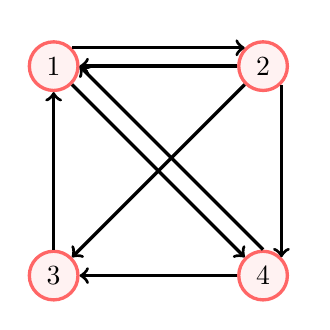
\begin{tikzpicture}[
        SIR/.style={circle, draw=red!60, fill=red!5, very thick, minimum size=5mm},
        node distance=2cm
        ]
        %Nodes
        \node[SIR]    (1)                              {1};
        \node[SIR]    (2)       [right=of 1] {2};
        \node[SIR]    (3)       [below=of 1] {3};
        \node[SIR]    (4)       [right=of 3] {4};
        
        %Lines
        \draw[->, very thick] (1.north east)  to node[above right] { } (2.north west);
        \draw[->, very thick] (1.south east)  to node[below right, sloped] { } (4.north west);
        \draw[->, very thick] (2.south east)  to node[right] { } (4.north east);
        \draw[->, very thick] (2.west)  to node[below right] { } (1.east);
        \draw[->, very thick] (3.north)  to node[right] { } (1.south);
        \draw[->, very thick] (2.south west)  to node[above left, sloped] { } (3.north east);
        \draw[->, very thick] (4.west)  to node[above right] { } (3.east);
        \draw[->, very thick] (4.north)  to node[above right, sloped] { } (1.east);
        \end{tikzpicture}
    \end{center}
    
The idea is to surf the web randomly (random walks on the graph) and if you do that long enough you will reach a \textbf{Steady state} where $\pi_i$ will be the probability of being on the i-th website.\\
In this case the vector $\underline{\pi} \in \mathbb{R}^4$ because there are 4 websites. 
\end{multicols}
We are assuming there are not separated sites. How can we represent the matrix? It an \textbf{Adjacency matrix}
\[
    \tilde{A} = \begin{bmatrix}
        0 & 1 & 1 & 1\\
        0 & 0 & 1 & 1\\
        1 & 0 & 0 & 0\\
        1 & 0 & 1 & 0\\
    \end{bmatrix}
    \rightarrow
    \tilde{A}_{ij} = \begin{cases}
        1 & \text{if there is a link from i to j}\\
        0 & \text{otherwise}
    \end{cases}    
    \hspace{0.5cm}
    \overset{\text{normalized version}}{\longrightarrow}
    A = \begin{bmatrix}
        0   & 1 & 1/3 & 1/2\\
        0   & 0 & 1/3 & 1/2\\
        1/2 & 0 & 0   & 0\\
        1/2 & 0 & 1/3 & 0\\
    \end{bmatrix}
\]
In the normalized version all columns sum up to 1. What happen if we multiply the matrix $A$ times a canonical basis vector $\underline{e}_3 = \begin{bmatrix}
    0 & 0 & 1 & 0
\end{bmatrix}^\intercal$?
\[
    A\underline{e_3} = \begin{bmatrix}
        1/3\\
        1/3\\
        0\\
        1/3\\
    \end{bmatrix}
\]
As it was trivial to figure, we obtain, in this case, the third column of the adjacency matrix. In a probability perspective, the vector $\underline{e}_3$ represents the probability of starting from the third website. The vector we obtain is the probability of reaching the other websites starting from the third one. This means that in this case we are certain that we start from the third website and for sure we won't be in that site in the following iteration. \\

Considering 
\[
\underline{\pi} = \begin{bmatrix}
    \pi_1\\
    \pi_2\\
    \pi_3\\
    \pi_4\\
\end{bmatrix}    
\]
The steady state is defined as: $A\underline{\pi} = \underline{\pi}$.
This means that, the steady state is the eigenvector of the matrix $A$ with eigenvalue 1. The matrix $A$ is positive (not positive-definite) i.e. it has all non-negative cohefficients. A positive matrix is denoted with $A > 0$.
From Perron-Frobenius theory we know that $\lambda_1 = 1$ is the largest eigenvalue.
\[
    \lambda_1 = 1 > \lambda_2 > \lambda_3 > \dots > \lambda_n \hspace{1cm} \lambda_i \neq 0
\] 
As mentioned in a previous lecture, we can use the power method in order to retrieve the largest eigenvalue. In particular, we start from:
\[
    \underline{\pi}^{(0)} \hspace{0.5cm}\text{with}\hspace{0.5cm} ||\underline{\pi}^{(0)}||=1    
\]
Then, for $k = 1, 2, \dots $
\[
    \underline{\pi}^{(k)} = \dfrac{A\underline{\pi}^{(k-1)}}{||A\underline{\pi}^{(k-1)}||}    
\]
\[
    \text{if } ||\underline{\pi}^{(k)} - \underline{\pi}^{(k-1)}|| < \epsilon \text{ then stop}    
\]
Obviously, $\epsilon$ represents a tolerance value. As we can see, there is an recursive definition in a sense that, at each iteration, the same operation is made on the same variable. For example:
\[
    \underline{\pi}^{(1)} = \dfrac{A\underline{\pi}^{(0)}}{||A\underline{\pi}^{(0)}||}    
    \hspace{2cm}
    \underline{\pi}^{(2)} = \dfrac{A\underline{\pi}^{(1)}}{||A\underline{\pi}^{(1)}||} = \dfrac{A^2\underline{\pi}^{()}}{||A^2\underline{\pi}^{(k-1)}||} 
\]
So, iterating k times:
\[
    \underline{\pi}^{(k)} = \dfrac{A^k\underline{\pi}^{(0)}}{||A^k\underline{\pi}^{(0)}||}     
\]
Since in $A$ there are no columns that are completely equal to 0, the matrix can be diagonalized. This implies that there are some $\underline{v}_i, i = 1, \dots, n$ that can used as a basis for the space. In particular we can write:
\[
    \underline{\pi}^{(0)} = \sum_{i=1}^n \alpha_i \underline{v}_i
\]
We want to plug this expression in the previous equation (power method). Before, notice that, $A\underline{v}_i = \lambda \underline{v}_i$ because $\underline{v}_i$ are the vectors which diagonalize $A$ so the ones such that $A = V\Lambda V^\intercal$. 
The numerator of $\underline{\pi}^{(k)}$ can be written as:
\[
    A^k \underline{\pi}^{(0)} = \alpha_1\lambda_1^k \left(\underline{v}_1 + \sum_{i=2}^{n} \dfrac{\alpha_i}{\alpha_1}\left(\dfrac{\lambda_i}{\lambda_1}\right)^k \underline{v}_i\right)    
\]
Proof:
\begin{multicols}{2}
    \[
    \begin{split}
        A^k \underline{\pi}^{(0)} &= V\Lambda^k V^{-1} \left(\alpha_1\underline{v}_1 + \dots + \alpha_n\underline{v}_n\right)\\
        &\overset{\circledast }{=} V\Lambda^k \left(\alpha_1\underline{e}_1 + \dots + \alpha_n\underline{e}_n\right)\\
        &= V\left(\alpha_1\lambda_1^k\underline{e}_1 + \dots + \alpha_n\lambda_n^k\underline{e}_n \right)\\
        &\overset{\diamond}{=} \alpha_1\lambda_1^k\underline{v}_1 + \dots + \alpha_n\lambda_n^k\underline{v}_n\\
        &= \alpha_1\lambda_1^k \left(\underline{v}_1 + \dfrac{\alpha_2}{\alpha_1}\left(\dfrac{\lambda_2}{\lambda_1}\right)^k \underline{v}_2 + \dots + \dfrac{\alpha_n}{\alpha_1}\left(\dfrac{\lambda_n}{\lambda_1}\right)^k \underline{v}_n\right)\\
    \end{split}
\]
\[
    \circledast  \rightarrow V^{-1}\underline{v}_i = V^{-1}\underline{v}_i = \begin{bmatrix}
        \horzbar & \underline{v}_1^\intercal & \horzbar\\
        \horzbar & \underline{v}_2^\intercal & \horzbar\\    
         & \vdots & \\
        \horzbar & \underline{v}_n^\intercal & \horzbar
    \end{bmatrix} \underline{v}_i
    = \underline{e}_i
\]
\[
    \diamond \rightarrow A\underline{v} = \lambda\underline{v} \implies AA\underline{v} = \lambda A\underline{v} \implies A^2\underline{v} = \lambda^2\underline{v}     
\]
\end{multicols}
If $k \to \infty$ then $\left(\dfrac{\lambda_i}{\lambda_1}\right)^k \to 0$ because $\lambda_1 > \lambda_i$ for $i = 2, \dots, n$ . So, the only remaining term is $\underline{v}_1$ which is the eigenvector with the largest eigenvalue. So what we have just done is the proof of the convergence of the power method.The closer are the eigenvalues to $\lambda_1$ the slower is the convergence.

   % lecture 8 absent because it was a lab
So far we have considered:
\[
    \underline{y} = X\underline{w} \hspace{1cm} X \in \mathbb{R}^{n \times p} \text{ and } \begin{Bmatrix}
        \text{Least Squares}: \underline{\hat{w}}_LS\\
        \text{Ridge Regression}: \underline{\hat{w}}_{RR}\\
    \end{Bmatrix} \underline{w} \in \mathbb{R}^p \text{ dense vector, i.e. not many zeros} 
\]
We are going to see a method which obtain a vector $\underline{\hat{w}}$ with many zeros, as sparse as possible. We want to consider this model:
\[
    \underline{y} = X\underline{w} \hspace{1cm} X \in \mathbb{R}^{n \times p} \hspace{1cm} p > n 
\]
We have said that the system is undetermined since it has infinite solutions. Suppose to have 2 features and 1 sample. 
\[
    X = \begin{bmatrix}
        2 & 3\\
    \end{bmatrix}
    \hspace{1cm}
    y = \begin{bmatrix}
        1\\
    \end{bmatrix}
\]
And so:
\[
    1 = \begin{bmatrix}
        2 & 3
    \end{bmatrix}\begin{bmatrix}
        w_1\\
        w_2
    \end{bmatrix} \implies
    1 = 2w_1 + 3w_2 \hspace{0.2cm} \leftarrow \hspace{0.2cm} \text{line}    
\]
As mentioned in a previous lecture, we want to find the minimum length solution so we can plot the line found before and the circles that represents the l2-norm distance.
\begin{center}
    \includegraphics[scale=0.6]{../images/LassoRidgePlot.png}
\end{center}
On the right-hand side it is represented the equivalent plot but with the l1-norm. We can see that the solution on the right has one coordinate (are features!) that is equal to zero. This is true in general, i.e. we will obtain sparser solution using the l1-norm rather than the l2-norm.\\
With L1-norm it's still a convex optimization problem and
\[
    F(\underline{w}) = ||X\underline{w} - \underline{y}||_2^2 + \lambda ||\underline{w}||_1    
\] 
This model is implemented by \textbf{Lasso} (Least Absolute Shrinkage and Selection Operator) and achieve both the shortest distance solution and the selection of some features.

This is important because by reducing the number of features, we increase the interpretability of the model.\\

There is also the \textbf{Elastic Net} which combines both Lasso and Ridge: 
\[
    F(\underline{w}) = ||X\underline{w} - \underline{y}||_2^2 + \lambda_1||\underline{w}||_1 + \lambda_2||\underline{w}||_2^2  
\] 

\vspace{2cm}
Once again, we start considering:
\[
    \underline{y} \in \mathbb{R}^n \hspace{1cm} X \in \mathbb{R}^{n \times p} \hspace{0.2cm} \text{with \emph{p} lin. ind. cols } (\implies \sigma_i > 0, \hspace{0.1cm} i = 1, \dots, p)  
\]
Now we write the formulation of the weights vector $w$ we found for Ridge Regression. 
\[
    \begin{split}
    \underline{\hat{w}}_R &= V\underbrace{(\Sigma^\intercal \Sigma + \lambda I)^{-1} \Sigma^\intercal}_{\substack{\Sigma^\intercal(\Sigma \Sigma^\intercal + \lambda I)^{-1}}} U^\intercal \underline{y}\\
    &= \underbrace{V\Sigma^\intercal U^\intercal}_{X^\intercal} \underbrace{U(\Sigma \Sigma^\intercal + \lambda I)^{-1} U^\intercal \underline{y}}_{\underline{\alpha} \in \mathbb{R}^n}\\
    &= X^\intercal \underline{\alpha}\\
    &= \sum_{i=1}^n \alpha_i \underline{x}_i\\
    \end{split}     
\]
In the second passage we have added the matrices $U^\intercal U$ because its the identity matrix. We obtain a weighted sum of the column vectors of $X^\intercal$, where $X$ is:
\[
X = \begin{bmatrix}
    \horzbar & \underline{x_1^\intercal} & \horzbar\\
    \horzbar & \underline{x_2^\intercal} & \horzbar\\    
     & \vdots & \\
    \horzbar & \underline{x_n^\intercal} & \horzbar
\end{bmatrix}
\]
So, until now, we have discussed about linear models. A generic form would be:
\[
    \hat{y}_i = w_1x_{i1} + w_2x_{i2} \hspace{1cm} \text{if} \hspace{1cm} \underline{x}_i = \begin{bmatrix}
        x_{i1}\\
        x_{i2}
    \end{bmatrix}    
\]
Now a new model:
\[
    \hat{y}_i = w_1x_{i1} + w_2x_{i2} + w_3x_{i1}^2 + w_4x_{i2}^2 + w_5x_{i1}x_{i2}    
\]
So, the original feature vector $\underline{x}$ is transformed into a new feature vector by means of function called feature map $\phi(x)$:
\[
    \phi(x) = \begin{bmatrix}
        x_1\\
        x_2\\
        x_1^2\\
        x_2^2\\
        x_1x_2
    \end{bmatrix} \in \mathbb{R}^d \hspace{1cm} d > p \text{ typically}    
\]
And
\[
    \hat{y}_i = \phi(x_i)^\intercal \underline{w}    
\]
In general $d$ can be huge.


\section{Kernel Methods}
The aim of this methods is to avoid the necessity of computing huge vectors.
\[
    \Phi =  \begin{bmatrix}
        \horzbar & \phi(\underline{x}_1)^\intercal & \horzbar\\
        \horzbar & \phi(\underline{x}_2)^\intercal & \horzbar\\    
         & \vdots & \\
        \horzbar & \phi(\underline{x}_n)^\intercal & \horzbar
    \end{bmatrix}
    \in \mathbb{R}^{n \times d} \hspace{1cm} \underline{\hat{y}} = \Phi \underline{w}
\]
The objective is still the same: i.e. finding $\underline{w}$. We are now going to consider ridge regression in order to achieve that. 
Instead of $\underline{\hat{w}}_R = X^\intercal \underline{\alpha}$ we can now write:
\[
    \underline{\hat{w}}_R = \Phi^\intercal \underline{\alpha}
\]
Where
\[
    \underline{\alpha} = U(\Sigma \Sigma^\intercal + \lambda I)^{-1} U^\intercal \underline{y} = (XX^\intercal + \lambda I)^{-1} \underline{y}    
\]
Here is the proof:
\[
    (U\Sigma V^\intercal V\Sigma^\intercal U^\intercal + \lambda UU^\intercal)^{-1} \underline{y}    
\]
Small recap considering both cases in which we consider both following cases: the features are on the horizontal axes and the vertical one.
\setlength{\columnseprule}{0.4pt}
\begin{multicols}{2}
    \[
        X \in \mathbb{R}^{n \times p} \hspace{0.2cm} \text{centered and } \begin{cases}
        n & \text{ \# of samples}\\
        p & \text{ \# of features}
    \end{cases}
    \]
    \[
        C = \dfrac{1}{n-1}X^\intercal X (spd)    
    \]
    can be factorized:
    \[
        C = V\Lambda V^\intercal    
    \]
    The columns of $V$ are the eigenvectors of $C$ and $\Lambda$ is a diagonal matrix with the eigenvalues of $C$. The eigenvectors are also called \textbf{principal directions}. The \textbf{principal components} instead, are obtained as:
    \[
        XV    
    \]
    And they represent the coordinates of the original samples in the new basis. If we write $X = U\Sigma V^\intercal$ then
    \[
        \begin{split}
            C &= \dfrac{1}{n-1}V\Sigma^\intercal U^\intercal U\Sigma V^\intercal \\
            &= \dfrac{1}{n-1}V\Sigma^2 V^\intercal \\
        \end{split}    
    \]
    And we have also that:
    \[
        \lambda_i = \dfrac{1}{n-1}\sigma_i^2    
    \]
    Moreover, with SVD:
    \[
        XV = U\Sigma V^\intercal V = U\Sigma    
    \]
    Are still principal components.
    \newcolumn
    \[
        X \in \mathbb{R}^{p \times n} \hspace{0.2cm} \text{centered and } \begin{cases}
        n & \text{ \# of samples}\\
        p & \text{ \# of features}
    \end{cases}
    \]
    Now, in this case we simply need to interchange the roles for $U$ and $V$.
    \[
        C = \dfrac{1}{n-1}XX^\intercal = \dfrac{1}{n-1}U\Sigma^2 V^\intercal
    \]
    The principal directions are in $U$ (and indeed not in $V$ this time). To get the principal components we have to:
    \[
        X^\intercal U    
    \]
\end{multicols}
In Ridge we have found that:
\[
\underline{\hat{w}}_{R} = \arg \min_{\underline{w}} ||\underline{y} - \Phi\underline{w}||_2^2 + \lambda ||\underline{w}||_2^2
\]
Let's consider a binary classification problem so we have ($\underline{x}_i, y_i$) and $y_i \in \{-1, 1\}, \underline{x}_i \in \mathbb{R}^p$. Now consider Least squares for this problem:
\vspace{2cm}    
To complete
\vspace{2cm}
\textbf{Example}
\[
    y_i = 1 \hspace{1cm} \underline{X}_i^\intercal \underline{w} = 100 \text{ for some } \underline{w}.     
\]









Consider $y = f: \mathbb{R}^n \to \mathbb{R}^m$ and the two cases: $\begin{cases}
    m \gg n\\
    m \ll n
\end{cases}$
In particular, the bottom case is the most interesting one to us since we might have many features in our model, especially for images and neural networks. For this case, the forward mode (FM) seen during last lecture is not very suitable because, considering NN, you need to compute a lot of derivatives wrt the weights. \\

Recall that, the Jacobian matrix is defined as:
\[
    \mathbf{J} = \begin{bmatrix}
        \dfrac{\partial y_1}{\partial x_1} & \dfrac{\partial y_1}{\partial x_2} & \dots & \dfrac{\partial y_1}{\partial x_n}\\
        \dfrac{\partial y_2}{\partial x_1} & \dfrac{\partial y_2}{\partial x_2} & \dots & \dfrac{\partial y_2}{\partial x_n}\\
        \vdots & \vdots & \ddots & \vdots\\
        \dfrac{\partial y_m}{\partial x_1} & \dfrac{\partial y_m}{\partial x_2} & \dots & \dfrac{\partial y_m}{\partial x_n}\\
    \end{bmatrix}    
\]
Suppose to have $\dot{\underline{X}} = \underline{e}_i$ as initialization value for the Wengert list forward pass method. We would have:
\[
    \dot{y}_j = \dfrac{\partial y_j}{\partial x_i} \hspace{0.3cm} j = 1, \dots, n    
\]
You obtain a column of the jacobian. In general we are interested in the product of the jacobian times a vector which could be anything but often is the evaluation of the function at the previous iteration. It means that in practical computation, we are not interested in having the jacobian and then to perform the matrix-vector multiplication, but we want the result of it. 
\[\mathbf{J}\underline{r}\]
\textbf{The FM of AD allows to have this result in a matrix free approach}. Any algorithm that is "matrix-free" means that in practise, even if the computation involves the presence of a matrix, you are able to avoid the construction of the complete matrix. You can resort to some tricks or algorithms that allow you to come up to the desired result without the need to explicitely computing the matrix. This is really good especially when dealing with big matrices. 

Instead of $\underline{\dot{X}} = \underline{e}_i$, we can start from $\underline{\dot{X}} = \underline{r}$ where $\underline{r}$ is the vector we want to multiply the jacobian with. 

\subsection{Dual-numbers}
They are similar to complex numbers. 
\[
    a + b\epsilon \hspace{0.3cm} \text{ with }\hspace{0.3cm} a,b \in \mathbb{R} \hspace{0.3cm} \text{and} \hspace{0.3cm} \epsilon \neq 0, \epsilon^2 = 0    
\]
Where $a$ is the real part and $b$ is the dual part. Basic operations with dual numbers:
\[
    (a + b\epsilon) + (c + d\epsilon) = (a + c) + (b + d)\epsilon    
\]
\[
    (a + b\epsilon)(c + d\epsilon) = ac + (ad + bc)\epsilon     
\]
Why this algebra is useful to our purposes? Consider the generic function $f$, we want to evaluate it with a dual number:
\[
    f(a + b\epsilon) = f(a) + f'(a)b\epsilon + \underbrace{\dfrac{f''(a)}{2}b^2\epsilon^2   + \dots}_{0}
\]
We have used the Taylor expansion, the last terms are zero because of $\epsilon^2$. Notice that, if we have unitary dual part ($b = 1$), we obtain the derivative of $f$ in $a$. This is the key point of the dual numbers:
\[
    b=1 \implies a + b\epsilon = a + \epsilon \implies f(a + \epsilon) = f(a) + f'(a)\epsilon    
\]
The last term is again a dual number in which the real part is the value of the function in $a$ and the dual part is the derivative of the function in $a$.\\

Let's check if the derivative properties are actually respected, suppose to have $f(x) = g(x)h(x)$:
\[
    \begin{split}
        f(a + \epsilon) &= g(a + \epsilon)h(a + \epsilon)\\
        &= [g(a) + g'(a)\epsilon][h(a) + h'(a)\epsilon]\\
        &= g(a)h(a) + g(a)h'(a)\epsilon + g'(a)h(a)\epsilon + g'(a)h'(a)\epsilon^2\\
        &= g(a)h(a) + \underbrace{[g(a)h'(a) + g'(a)h(a)]}_{\text{der. of the product}}\epsilon\\
    \end{split}
\]
Or $f(x) = g(h(x))$:
\[
    \begin{split}
        f(a + \epsilon) &= g(h(a + \epsilon))\\
        &= g(h(a) + h'(a)\epsilon)\\
        &= \underbrace{ g(h(a))}_{f(a)} + \underbrace{g'(h(a))h'(a)\epsilon}_{f'(a)\epsilon}\\        
    \end{split}
\]
Numerical example:  
\[
    f(x) = \dfrac{1}{x} \implies f(x+ \epsilon) = \dfrac{1}{x + \epsilon} = \dfrac{x -\epsilon}{(x + \epsilon)(x - \epsilon)} = \dfrac{x - \epsilon}{x^2 - \epsilon^2} = \dfrac{x - \epsilon}{x^2} = \underbrace{\dfrac{1}{x}}_{f(a)} - \underbrace{\dfrac{1}{x^2}\epsilon}_{f'(a)\epsilon}    
\]
Normally, we won't use the definition like this, but we will use real values, i.e. $x = 2$ for example. There is formalism for which $\epsilon$ are represented as matrices:
\[
    \epsilon = \begin{bmatrix}
        0 & 1\\
        0 & 0
    \end{bmatrix}
    \hspace{0.3cm} \implies \hspace{0.3cm}
    \epsilon^2 = \begin{bmatrix}
        0 & 1\\
        0 & 0
    \end{bmatrix}
    \begin{bmatrix}
        0 & 1\\
        0 & 0
    \end{bmatrix}
    = \begin{bmatrix}
        0 & 0\\
        0 & 0
    \end{bmatrix}    
\]
But this is not so important because at the end we are interested in its cohefficients. 

Let's now analyze the \textbf{Backward or reverse mode}.\\
It's related with the sensitivity of the output wrt the input. We introduce a new quantity:
\[
    \overline{v}_i = \dfrac{\partial y}{\partial v_i}   
\]
Where $v_i$ is one of the variables we have written considering the forward mode and which might not be the input. This is what happen in backpropagation, a partial derivative of the output wrt to a certain weight of the NN.\\
We start from the output:
\begin{center}
    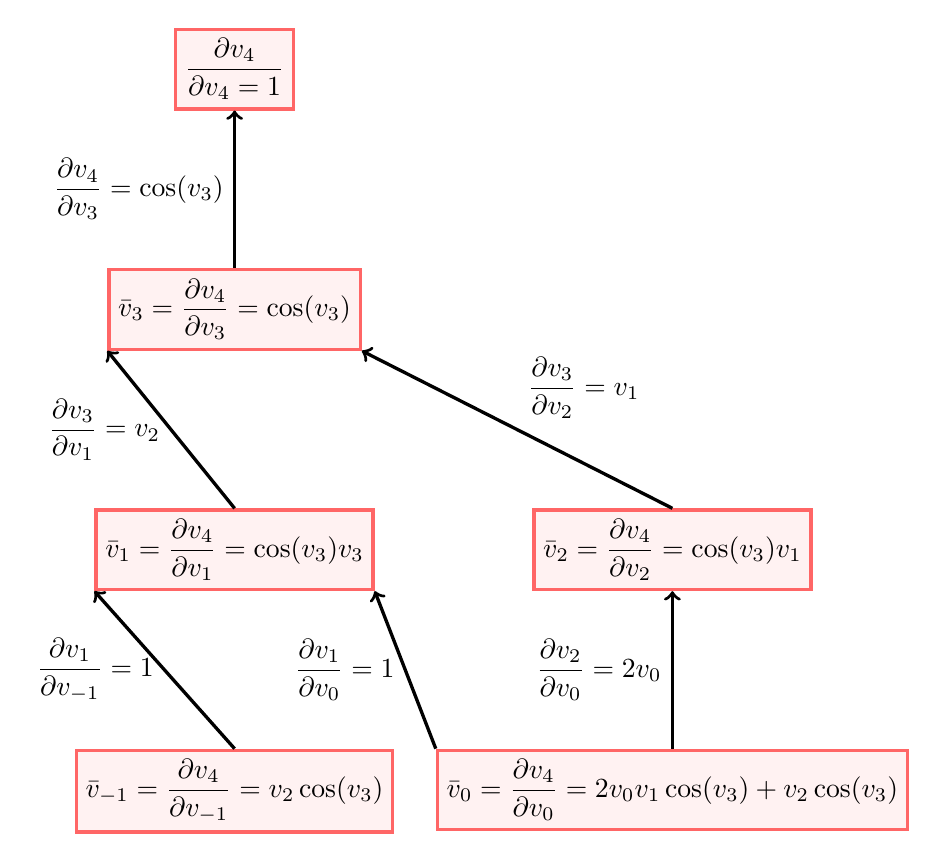
\begin{tikzpicture}[
        SIR/.style={draw=red!60, fill=red!5, very thick, minimum size=5mm},
        node distance=2cm
        ]
        %Nodes
        \node[SIR]    (1)                    {$\dfrac{\partial v_4}{\partial v_4 = 1}$};
        \node[SIR]    (2)       [below=of 1] {$\bar{v}_3 = \dfrac{\partial v_4}{\partial v_3} = \cos(v_3)$};
        \node[SIR]    (3)       [below=of 2] {$\bar{v}_1 = \dfrac{\partial v_4}{\partial v_1} = \cos(v_3)v_3$};
        \node[SIR]    (4)       [right=of 3] {$\bar{v}_2 = \dfrac{\partial v_4}{\partial v_2} = \cos(v_3)v_1$};
        \node[SIR]    (5)       [below=of 3] {$\bar{v}_{-1} = \dfrac{\partial v_4}{\partial v_{-1}} = v_2\cos(v_3)$};
        \node[SIR]    (6)       [below=of 4] {$\bar{v}_0 = \dfrac{\partial v_4}{\partial v_0} = 2v_0v_1\cos(v_3) + v_2\cos(v_3)$};
        
        %Lines
       \draw[->, very thick] (2.north)  to node[left] {$\dfrac{\partial v_4}{\partial v_3} = \cos(v_3)$} (1.south);
       \draw[->, very thick] (3.north)  to node[left] {$\dfrac{\partial v_3}{\partial v_1} = v_2$} (2.south west);
        \draw[->, very thick] (4.north)  to node[above right] {$\dfrac{\partial v_3}{\partial v_2} = v_1$} (2.south east);
        \draw[->, very thick] (5.north)  to node[left] {$\dfrac{\partial v_1}{\partial v_{-1}} = 1$} (3.south west);
        \draw[->, very thick] (6.north)  to node[left] {$\dfrac{\partial v_2}{\partial v_0} = 2v_0$} (4.south);
        \draw[->, very thick] (6.north west)  to node[left] {$\dfrac{\partial v_1}{\partial v_0} = 1$} (3.south east);
       \end{tikzpicture}
\end{center}
Where the bottom left box is $\frac{\partial y}{\partial x_{1}}$ and the bottom right box is $\frac{\partial y}{\partial x_{2}}$
We have been able to compute all the intermediate sensitivities not just wrt of the imput. If we have $\mathbb{R}^n \to \mathbb{R}^m$ and $n \gg m$ this method is very efficient because with just one sweep you compute the derivative of the output wrt all the input parameters. In the forward mode i would have had to perform $n$ forward steps, and obviously this would be more costly.

\section{Convolution}
In this lecture we are going to deal with the topic of convolution. The general definition is given by:
\[
    (f*g)(x) = \int_{-\infty}^{+\infty} f(t)g(x-t)dt    
\]
The operation can be applied also to vector with:
\[
    (\underline{c}*\underline{d})_K = \sum_{i+j = k} c_i d_j = \sum_i c_i d_{k-i}    
\]
The pedix $K$ is used to indicate the $k$-th element of the vector to which is the convolution is applied. The vectors can be expressed also as polynomials:
\[
    c(x) = c_0 + c_1 x + c_2 x^2 + \dots + c_{n-1} x^{n-1}    
\]
\[
    d(x) = d_0 + d_1 x + d_2 x^2 + \dots + d_{n-1} x^{n-1}
\]
The convolution is the product of these polynomials. [to finish]


\subsection{Cyclic convolution}
The cyclic convolution is a particular case of convolution in which the vectors are cyclic. This means that the last element of the vector is followed by the first one. The cyclic convolution is defined as:
\[
    (\underline{c}\circledast \underline{d})_K = \sum_{i+j = k \mod(n)} c_i d_j 
\]
How can this be written in matrix form?
\begin{multicols}{2}
    \begin{center}
        \textsc{Convolution}
    \end{center}
    In this case are used the \textbf{Toeplitz matrices} (or also called Time-Invariant Linear Systems), the elements are given by $(2n - 1)$-length sequence:
    \[
        \left\{t_K: -(n-1) \leq K \leq (n-1) \right\}    
    \]
    The element in position $(i,j)$ is given by $T(i,j) = t_i - t_j$ and the generic Toeplitz matrix as this shape:
    \[
        T = \begin{bmatrix}
            t_0 & t_{-1} & t_{-2} & \dots & t_{-(n-1)} \\
            t_1 & t_0 & t_{-1} & \dots & t_{-(n-2)} \\
            t_2 & t_1 & t_0 & \dots & t_{-(n-3)} \\
            \vdots & \vdots & \vdots & \ddots & \vdots \\
            t_{n-1} & t_{n-2} & t_{n-3} & \dots & t_0
        \end{bmatrix}    
    \]
    So, it's easy to notice that on the diagonal there is always a constant vector.
    \newcolumn
    \begin{center}
        \textsc{Cyclic convolution}
    \end{center}
    In this case are used the \textbf{Circulant matrices}, a particular case of a Toeplitz matrix. For a given $n \times n$ matrix, the elements are given by $(n)$-length sequence:
    \[
        \left\{c_K: 0 \leq K \leq (n-1) \right\}
    \]
    The element in position $(i,j)$ is given by $C(i,j) = c_{i-j \mod(n)}$ and the generic Circulant matrix as this shape:
    \[
        C = \begin{bmatrix}
            c_0 & c_{n-1} & c_{n-2} & \dots & c_1 \\
            c_1 & c_0 & c_{n-1} & \dots & c_2 \\
            c_2 & c_1 & c_0 & \dots & c_3 \\
            \vdots & \vdots & \vdots & \ddots & \vdots \\
            c_{n-1} & c_{n-2} & c_{n-3} & \dots & c_0
        \end{bmatrix}
    \]
    As you can see, the last element of a column vector becomes the first element of the next column vector, for this reason is called circulant. 
\end{multicols}
Example of circulant matrix:
\[
    C = \begin{bmatrix}
        1 & 8 & 5 & 3\\
        3 & 1 & 8 & 5\\
        5 & 3 & 1 & 8\\
        8 & 5 & 3 & 1
    \end{bmatrix}    
\]
Now we introduce a \textbf{permutation matrix} $P$ defined as follows:
\[
    P = \begin{bmatrix}
        0 & 1 & 0 & 0\\
        0 & 0 & 1 & 0\\
        0 & 0 & 0 & 1\\
        1 & 0 & 0 & 0
    \end{bmatrix}
\]
If we multiply the permutation matrix with a vector, this happen:
\[
    P \underline{c} = \begin{bmatrix}
        0 & 1 & 0 & 0\\
        0 & 0 & 1 & 0\\
        0 & 0 & 0 & 1\\
        1 & 0 & 0 & 0
    \end{bmatrix} \begin{bmatrix}
        c_0\\
        c_1\\
        c_2\\
        c_3
    \end{bmatrix} = \begin{bmatrix}
        c_1\\
        c_2\\
        c_3\\
        c_0
    \end{bmatrix}    
\]
All elements are shifted of 1 position. This means that the circulant matrix $C$ can be built as follows:
\[
    C = c_0 I + c_1 P + c_2 P^2 + c_3 P^3    
\]
This is true for any circulant matrix so we define also $D$:
\[
    D = d_0 I + d_1 P + d_2 P^2 + d_3 P^3 
\]
What happen when we multiply $CD$, i.e two circulant matrices?
\[
    CD = (c_0 I + c_1 P + c_2 P^2 + c_3 P^3)(d_0 I + d_1 P + d_2 P^2 + d_3 P^3)
\]
But this means that we end up with elements with $P^4$ and $P^5$ and so on, but $P^4 = I$, $P^5 = P$ and $P^6 = P^2$. This makes sense even considering that we are dealing with circulant matrices. In general we can say:
\[
    P_n \text{ of } n \times n \implies P^n = I    
\]

\noindent \textbf{Example:}\\
We want to multiply (1,2,1)(3,1,2). We transform the two vectors in two polynomials:
\[
    (1 + 2x + x^2)(3 + x + 2x^2) = 3 + 7x + 7x^2 + 5x^3 + 2x^4    
\]
The terms at the third and forth power must be shifted. 
\[
    (3 + 5) + (7 + 2)x + 7x^2 = 8 + 9x + 7x^2     
\]
The final result is (8,9,7) and, to check its correctness we can consider this sort of property:
\[
    \{(1,2,1) \implies 1+2+1 =4 \times 6 = 3+1+2 \Longleftarrow  (3,1,2) \} \implies 6 \times 4 = 8+9+7 \Longleftarrow  (8,9,7)     
\] 
If we now rename the vectors $\underline{c} = (1,2,1)$ and $\underline{d} = (3,1,2)$, we can compute their convolution by:
\[
    \underline{c} * \underline{d} =     
C\underline{d} = \begin{bmatrix}
        1 & 1 & 2\\
        2 & 1 & 1\\
        1 & 2 & 1
    \end{bmatrix} \begin{bmatrix}
        3\\
        1\\
        2
    \end{bmatrix} = \begin{bmatrix}
        3+1+4\\
        6+1+2\\
        3+2+2
    \end{bmatrix} = \begin{bmatrix}
        8\\
        9\\
        7
    \end{bmatrix}
\]
We have built the circulant matrix starting from the vector $\underline{c}$ and then we have multiplied it with the vector $\underline{d}$. This is the same as multiplying the two polynomials. I did not understand wheter you can either build $C$ from using the initial vector as its row or column.

The matrix $CD$ is circulant because it's the product of two circulant matrices. 

\subsection{Eigenvectors and eigenvalues of a circuland matrix}
Let's start considering again the permutation matrix $P$. We can compute its eigenvalues by using the definition method:
\[
    P - \lambda I = \begin{bmatrix}
        -\lambda & 1 & 0 & 0\\
        0 & -\lambda & 1 & 0\\
        0 & 0 & -\lambda & 1\\
        1 & 0 & 0 & -\lambda
    \end{bmatrix}
    \implies
    \det(P - \lambda I) = \lambda^4 - 1 = 0
\]
\newpage
So the eigenvalues of $P$ are the fourth roots of 1, which correspond to:
\begin{multicols}{2}
    \begin{center}
        \includegraphics[scale = 0.4]{../images/FourthRoots.jpg}
    \end{center}
    \newcolumn
    \vspace{0.2cm}
    \[
        \begin{split}
            &\lambda^4 - 1 = 0\\
            &\lambda_1 = 1\\
            &\lambda_2 = i\\
            &\lambda_3 = -1\\
            &\lambda_4 = -i
        \end{split}    
    \]
\end{multicols}
We introduce now the complex number $w$ given by:
\[
    w = e^{\dfrac{2\pi i}{n}} \overset{\text{in this case}}{\longrightarrow}    w = e^{\dfrac{2\pi i}{4}} \implies \begin{cases}
        \lambda_1 = w^0\\
        \lambda_2 = w^1\\
        \lambda_3 = w^2\\
        \lambda_4 = w^3
    \end{cases}
\]
In general we have:
\[
    P_n \implies \lambda^n - 1 = 0 \implies w^0, w^1, \dots, w^{n-1}
\]
Another property of $P$: it's orthogonal indeed $P^\intercal P = I$.
What about the eigenvectors of $P$? Consider the generic matrix $C$ written in terms of $P$:
\[
    C = c_0 I + c_1 P + c_2 P^2 + c_3 P^3    
\]
We want to find the eigenvectors of $C$. If $\lambda_k, \underline{v}_k$ is the couple of eigenvalue and eigenvector of $C$, then:
\[
    \begin{split}
        C\underline{v}_k &= \lambda_k \underline{v}_k\\
        (c_0 I + c_1 P + c_2 P^2 + c_3 P^3)\underline{v}_k &= (c_0 + c_1 \lambda_k + c_2 \lambda_k^2 + c_3 \lambda_k^3)\underline{v}_k\\
    \end{split}
\]
$\underline{v}_k$ is an eigenvector of $P$.\\

\noindent \textbf{Example:}\\
\begin{multicols}{4}
    \[
        \begin{split}
            \lambda_1 &= 1\\
            \underline{v}_1 &= \begin{bmatrix}
                1\\
                1\\
                1\\
                1
            \end{bmatrix}    
        \end{split} 
    \]
    \[
        \begin{split}
            \lambda_2 &= i\\
            \underline{v}_2 &= \begin{bmatrix}
                1\\
                i\\
                i^2\\
                i^3
            \end{bmatrix}    
        \end{split} 
    \]
    \[
        \begin{split}
            \lambda_3 &= -1\\
            \underline{v}_3 &= \begin{bmatrix}
                -1\\
                1\\
                -1\\
                1
            \end{bmatrix}    
        \end{split} 
    \]
    \[
        \begin{split}
            \lambda_4 &= -i\\
            \underline{v}_4 &= \begin{bmatrix}
                1\\
                (-i)\\
                (-i)^2\\
                (-i)^3
            \end{bmatrix}    
        \end{split} 
    \]
\end{multicols}    
Example of computation of the third eigenvector:
\[
    \underline{v}_3 = 
    \underbrace{
    \begin{bmatrix}
        0 & 1 & 0 & 0\\
        0 & 0 & 1 & 0\\
        0 & 0 & 0 & 1\\
        1 & 0 & 0 & 0
    \end{bmatrix}   
    \begin{bmatrix}
        1\\
        -1\\
        1\\
        -1
    \end{bmatrix}}_{\begin{bmatrix}
        -1\\
        1\\
        -1\\
        1\\
    \end{bmatrix}}
    = \underbrace{-1
    \begin{bmatrix}
        1\\
        -1\\
        1\\
        -1
    \end{bmatrix}}_{\begin{bmatrix}
        -1\\
        1\\
        -1\\
        1\\
    \end{bmatrix}}
\]
We define 
\[
    \mathbf{F} = \underbrace{\begin{bmatrix}
        1 & 1 & 1 & 1\\
        1 & w & w^2 & w^3\\
        1 & w^2 & w^4 & w^6\\
        1 & w^3 & w^6 & w^9
    \end{bmatrix}}_{\text{eigenvectors}}    
    \underbrace{\dfrac{1}{\sqrt{n}}}_{\text{normalization}} \hspace{0.3cm} \text{where} \hspace{0.3cm} w = e^{\dfrac{2\pi i}{4}}
\]
If you multiply a vector for $\mathbf{F}$ you get its \textbf{Discrete Fourier Transform (DFT)}.
\[
    \underline{\lambda}_c = \begin{bmatrix}
        \lambda_0(c)\\
        \vdots\\
        \lambda_{K-1}(c)
    \end{bmatrix}    
    = 
    \begin{bmatrix}
        c_0 + c_1 + \dots + c_{n-1}\\
        \vdots\\
        c_0 + c_1w^{n-1} + \dots + c_{n-1}w^{(n-1)(n-1)}
    \end{bmatrix}
    =
    \mathbf{F} \begin{bmatrix}
        \underline{c}_0\\
        \vdots\\
        \underline{c}_{n-1}
    \end{bmatrix}
    = \mathbf{F}\underline{c}
\]
Where $\underline{\lambda}_c$ is the vector containing the eigenvalues of the circulant matrix $C$ and $\underline{c}$ is the vector containing the coefficients of the polynomial $c(x)$.\\

Consider two matrices $A$ and $B$, with some eigenvalues and eigenvectors:
\[
    A\underline{v} = \lambda \underline{v} \hspace{0.5cm} B\underline{v} = \gamma \underline{v}    
\]
then
\[
    AB\underline{v} = \gamma A\underline{v} = \gamma \lambda \underline{v}     
\]
So the eigenvalues of the product is the product of the eigenvalues. Now we are going to exploit this property: consider two circulant matrices $C$ and $D$ built from the vectors $\underline{c}$ and $\underline{d}$:
\begin{itemize}
    \item $CD$ in the first row you have the cyclic convolution of $\underline{c}$ and $\underline{d}$ ($\underline{c} \circledast \underline{d}$)
    \item $\mathbf{F}(\underline{c} \circledast \underline{d})$ is the vector of eigenvalues of $CD$
\end{itemize}
Eigenvalues of $C$: $\lambda(c) = \mathbf{F}\underline{c}$ and eigenvalues of $D$: $\lambda(d) = \mathbf{F}\underline{d}$\\
So the eigenvalues of $CD$ are:
\[
    \lambda(CD) = \lambda(C) \cdot^* \lambda(D)= \mathbf{F}\underline{c} \cdot^* \mathbf{F}\underline{d} = \underline{\lambda}_{CD}
\]
Two ways of computing the eigenvalues:
\[
    \mathbf{F}(\underline{C} \circledast \underline{d}) = \mathbf{F}\underline{c} \cdot^* \mathbf{F}\underline{d}
\]
This is called \textbf{Convolution rule}. Which is the fastest method?
The FFT (Fast Fourier Transform) takes $n\log(n)$ operations for computing the matrix multiplication.
\begin{itemize}
    \item $\mathbf{F}(\underline{C} \circledast \underline{d}) = n^2 n\log(n)$
    \item $\mathbf{F}\underline{c} \cdot^* \mathbf{F}\underline{d} = 2n\log(n) + n$ \hspace{0.3cm }so it's better this one!
\end{itemize}
So far we have seen that our goal is to find:
\[
    \underline{w}^* = \arg \min_{\underline{w}} J(\underline{w})   
\]
Let's now see gradually, how to solve this minimization problem by means of different methods.

\section{Gradient descent (GD)}
Consider the following first order approximation:
\[
    \Delta J \approx \nabla J \underbrace{\Delta \underline{w}}_{\Delta \underline{w} = -\eta\nabla J} = -\eta \|\nabla J\|^2    
\]
The actual method is defined by the formula:
\[
     \underline{w}^{(k+1)}= w^{(k)}- \eta\nabla J(\underline{w}^{(k)})   
\]
Let's see some properties using now $x$ as $w$, so the formula is: $ \underline{x}^{(k+1)}= x^{(k)}- \eta\nabla f(\underline{x}^{(k)}) $ where $f$ is the function we want to minimize and $\eta$ the learning rate.

If $\eta$ is to small, the convergence is slow. If $\eta$ is too large, the convergence is not guaranteed since you have overshooting. For now, we are considering a fixed $\eta$ (not dependent on $k$).

\subsection{Convergence}
Definition: $f: \text{dom}(f) \to \mathbb{R}$ is \textbf{convex} if:
\begin{enumerate}[i]
    \item $\text{dom}(f)$ is convex
    \item $\forall \underline{x}, \underline{y} \in \text{dom}(f), \lambda \in [0,1]: f(\lambda \underline{x} + (1-\lambda)\underline{y}) \leq \lambda f(\underline{x}) + (1-\lambda)f(\underline{y})$
\end{enumerate} 
Lemma: if $\text{dom}(f)$ is open and $f$ is differentiable, then $f$ is complex iff the domain of $f$ is convex and 
\[
    f(\underline{y}) \geq f(\underline{x}) + \nabla f(\underline{x})^T(\underline{y}-\underline{x}) \quad \forall \underline{x}, \underline{y} \in \text{dom}(f)    
\]
This last formulation states that the function must be above the tangent line or, more generally, above the tangent hyperplane built starting from point \underline{x}.\\

Set $\underline{x} = \underline{x}^{(k)}$ and $\underline{y} = \underline{x}^*$, where $\underline{x}^*$ is the minimum point. Then we can substitute the inequality in the lemma and obtain:
\[
    \begin{split}
        f(\underline{x}^*) &\geq f(\underline{x}^{(k)}) + \nabla f(\underline{x}^{(k)})^T(\underline{x}^*-\underline{x}^{(k)})\\
        f(\underline{x}^{(k)}) - f(\underline{x}^*) &\leq \nabla f(\underline{x}^{(k)})^T(\underline{x}^*-\underline{x}^{(k)})
    \end{split}
\]
We define now the value $\underline{g}^{(k)} = \nabla f(x^{(k)})$. Thanks to this, we can rewrite the original gradient descent formula as:
\[
    \underline{x}^{(k+1)} -\underline{x}^{(k)}= - \eta \underline{g}^{(k)}    
\]
And so we can reformulate as follows:
\[
    \underline{g}^{(k)} = \frac{\underline{x}^{(k+1)} -\underline{x}^{(k)}}{-\eta} = \frac{\underline{x}^{(k)} - \underline{x}^{(k+1)}}{\eta}
\]
Thanks to this we have:
\[
    f(\underline{x}^{(k)}) - f(\underline{x}^*) \leq \nabla f(\underline{x}^{(k)})^T(\underline{x}^*-\underline{x}^{(k)}) = \dfrac{1}{\eta} (\underline{x}^{(k)} - \underline{x}^*)(\underline{x}^{(k)}-\underline{x}^{(k+1)}) = (\star)
\]
We are now going to exploit a property seen also when dealing with least squares, for which:
\[
    \|\underline{v} - \underline{w}\|^2 = (\underline{v} - \underline{w})^\intercal (\underline{v} - \underline{w}) = \underline{v}^\intercal \underline{v} - 2\underline{v}^\intercal \underline{w} + \underline{w}^\intercal \underline{w} = \|\underline{v}\|^2 - 2\underline{v}^\intercal \underline{w} + \|\underline{w}\|^2    
\]
\[
    \implies 2\underline{v}^\intercal \underline{w} = \|\underline{v}\|^2 + \|\underline{w}\|^2 - \|\underline{v} - \underline{w}\|^2    
\]
We reconduct to this form by adding a 2 both at the numerator and denumerator and considering the two parenthesis as the vectors $v$ and $w$:
\[
    \begin{split}
        (\star) &= \dfrac{1}{2 \eta} 2\underbrace{(\underline{x}^{(k)} - \underline{x}^*)}_{\underline{v}^\intercal}\underbrace{(\underline{x}^{(k)}-\underline{x}^{(k+1)})}_{\underline{w}} \\
        &= \dfrac{1}{2 \eta} \left(\|\underline{x}^{(k)} - \underline{x}^{(k+1)}\|^2 + \|\underline{x}^{(k)} - \underline{x}^*\|^2 - \|\underline{x}^{(k+1)} - \underline{x}^*\|^2 \right) \\
        &= \dfrac{1}{2 \eta} \left( \eta^2 \|\underline{g}^{(k)}\|^2 + \|\underline{x}^{(k)} - \underline{x}^*\|^2 - \|\underline{x}^{(k+1)} - \underline{x}^*\|^2 \right) \\
        &= \dfrac{\eta}{2} \|g^{(k)}\| + \dfrac{1}{2 \eta} \left( \|\underline{x}^{(k)} - \underline{x}^*\|^2 - \|\underline{x}^{(k+1)} - \underline{x}^*\|^2 \right) \\
    \end{split}
\]
In the second row, in the last norm, you should have $x^{(k)}$ also (notice the property) but it's not there because it's summed to it's opposite so they cancel out.\\ 
If $N$ is the last iteration we want to perform we can write:
\[
    \sum_{k=0}^{N-1}   \left(f(\underline{x}^{(k)})-f(\underline{x}^*)\right) \leq \dfrac{\eta}{2} \sum_{k=0}^{N-1}\|\underline{g}^{(k)}\|^2 + \dfrac{1}{2 \eta}\|\underline{x}^{(0)} - \underline{x}^*\|^2  = (\divideontimes)
\]
There are just two terms of $\underline{x}$ because it is a telescopic sum and the intermediate contributions cancel out (see previous equations in which both termns $x^{(k)}$ and $x^{(k+1)}$ are present). To be even more precise, there should be also another term $x^{(N)}$ (its norm with x star)but it is not there because it is summed with the negative sign so, the inequality holds even without it.

Recall that $x^{(0)}$ is the initial guess, given. The problem is the norm of the gradient, which is not known. 

\subsection{Lipschitz convex functions}
We are assuming that all the gradients are bounded ($\|\underline{g}^{(k)} \leq L\|, \forall k$) which implies that the function is Lipschitz continuous. We want to prove this theorem:

\textbf{Theorem}: $f:\mathbb{R}^d \to \mathbb{R} $ convex, differentiable with minimum $\underline{x}^*$, suppose that $\|x^{(0)} - x^*\| < R$ and $\nabla f(x) \leq L$. Then chosing $\eta = \frac{R}{L\sqrt{N}}$ we have 
\[
    \dfrac{1}{N}    \sum_{k=0}^{N-1} \left(f(\underline{x}^{(k)})-f(\underline{x}^*)\right) \leq \dfrac{RL}{\sqrt{N}}
\]
For example the function $f(x) = x^2$ does not satisfy the hypothesis of this theorem because the gradient is not bounded. This hypothesis $\|x^{(0)} - x^*\| < R$ states that the initial guess is not too far from the optimum. 
Let's now consider the quantity $(\divideontimes)$, it can be rewritten, considering the hypothesis of the theorem, as:
\[
    (\divideontimes) = \underbrace{\dfrac{\eta}{2}NL^2 + \dfrac{1}{2\eta}R^2}_{l(\eta)} \hspace{0.5cm} \implies \hspace{0.5cm} l'(\eta) = \dfrac{NL^2}{2} - \dfrac{R^2}{2\eta^2}   
\]
We set the derivative to zero to find the minimum of the function $l(\eta)$:
\[
    NL^2 - \dfrac{R^2}{\eta^2} = 0 \hspace{0.5cm} \implies \hspace{0.5cm} \eta = \dfrac{R}{L\sqrt{N}}    
\]
Which corresponds to the value we have stated in the hypothesis of the theorem. We now substitute the value of $\eta$ in $l(\eta)$:
\[
    l(\eta) = \dfrac{\eta}{2}NL^2 + \dfrac{1}{2\eta}R^2 = \dfrac{R}{2L\sqrt{N}}NL^2 + \dfrac{1}{2}\dfrac{R^2 L\sqrt{N}}{R} = RL{\sqrt{N}}
\]
So, we recap what we have done so far:
\[
    \begin{split}
        \sum_{k=0}^{N-1} \left(f(\underline{x}^{(k)})-f(\underline{x}^*)\right) &\leq \dfrac{\eta}{2} \sum_{k=0}^{N-1}\|\underline{g}^{(k)}\|^2 + \dfrac{1}{2 \eta}\|\underline{x}^{(0)} - \underline{x}^*\|^2  = \dfrac{\eta}{2}NL^2 + \dfrac{1}{2\eta}R^2\\
        &\leq \dfrac{\eta}{2}NL^2 + \dfrac{1}{2\eta}R^2\\
        &\leq RL{\sqrt{N}}
    \end{split}
\]
We can divide both terms for $N$ and obtain the result:
\[
    \dfrac{1}{N} \sum_{k=0}^{N-1} \left(f(\underline{x}^{(k)})-f(\underline{x}^*)\right) \leq \dfrac{RL}{\sqrt{N}}    
\]
The left part is a sort of average of the error, we can bound it by working on the right part. 
\[
    \dfrac{RL}{\sqrt{N}} \leq \epsilon \implies \dfrac{R^2L^2}{N} \leq \epsilon^2 \implies N \geq \dfrac{R^2L^2}{\epsilon^2}    
\]
And so $N = O(\frac{1}{\epsilon^2})$. This is the number of iterations of the gradient descent method that we need in order to achieve an average error $\epsilon$. $R,L$ are not quantity easily computable but $R$ in general, in real scenarios, could be big (look how it is defined in the theorem). $L$ also can be big. An \textbf{important} thing to notice regarding the last result is that we have found a bound which does not depend on the dimension of the feature vector $d$ (indeed we defined $f: \mathbb{R}^d \to \mathbb{R}$).

\subsection{Smooth convex functions}
Definition: $f: \text{dom}(f) \to \mathbb{R}$ differentiable, $X \subseteq \text{dom}(f)$ is convex, $L \in \mathbb{R}^+$ (is a positive constant) function $f$ is smooth with parameter $L$ over $X$ if:
\[
    \forall \underline{x}, \underline{y} \in X: f(\underline{y}) \leq f(\underline{x}) + \nabla f(\underline{x})^T(\underline{y}-\underline{x}) + \dfrac{L}{2}\|\underline{y}-\underline{x}\|^2    
\]
This means that the function is below a quadratic approximation. \\

\textbf{Lemma}: dom($f$) is open and convex and $f: \text{ dom}(f) \to \mathbb{R}$ differentiable. Let $L \in \mathbb{R}^+$ the following statements are equivalent:
\begin{enumerate}
    \item $f$ is smooth with paramenter $L$ over dom($f$)
    \item $g$ defined by $\underline{g}(\underline{x}) = \dfrac{L}{2}\underline{x}^\intercal \underline{x} - f(x)$ is convex over $\text{dom}$(\underline{g}) = dom($f$) 
\end{enumerate}
Considering the definition given above we have these cases:
\begin{itemize}
    \item if $L=0$ we can rewrite the inequality as:
    \[
        f(\underline{y}) = f(\underline{x}) + \nabla f(\underline{x})^T(\underline{y}-\underline{x})      
    \]
    Which is the definition of affine function.
    \item if $f(x) = x^2$, i.e. a function which does not satisfy the hypothesis of the theorem:
    \[
        f(y) = y^2 = x^2 + 2x(y - x)+(y- x)^2    
    \]
    Where there should be a $\frac{L}{2}$ in front of the last term but it is not there because it is 1 which implies that $L=2$. So, the function is convex and smooth with parameter $L=2$.
    \item if $f(\underline{x}) = \underline{x}^\intercal Q \underline{x} + \underline{b}^\intercal \underline{x} + c$, typical exmaple of quadratic function. $Q$ is a $d \times d$ matrix , symmetric, $\underline{b} \in \mathbb{R}^d$ and $c \in \mathbb{R}$. The function is smooth with $L = 2\|Q\|$ (twice the spectral norm). Where:
    \[
        \|Q\| = \max_{\overset{\underline{x} \in \mathbb{R}^d}{\underline{x}\neq 0}} \dfrac{\|A\underline{x}\|}{\|\underline{x}\|}   
    \]
    \item if $f(x) = x^4$ then $f$ is not smooth but is convex. \textbf{You cannot expect functions that have an asymptotic behaviour higher the quadratic one which are smooth. The highest degree for which you can expect to have smoothness is 2. This does not imply that the functions with degree lower than 2 are smooth.} Consider for example $f(x)= |x|^{3/2}$.
\end{itemize}

\textbf{Lemma}: $f: \mathbb{R}^d \to \mathbb{R}$ convex, differentiable. The following statements are equivalent:
\begin{enumerate}
    \item $f$ is smooth with parameter $L$ over dom($f$)
    \item $\forall \underline{x}, \underline{y} \in \mathbb{R}^d: \|\nabla f(\underline{x}) - \nabla f(\underline{y})\| \leq L\|\underline{x} - \underline{y}\|$
\end{enumerate}
So if the gradient is Lipschitz continuous, then the function is smooth and viceversa.\\

Let $f: \mathbb{R}^d \to \mathbb{R}$ smooth L, differentiable. Picking $\eta = \frac{1}{L}$, Gradient descent satisfies:
\[
    f(\underline{x}^{(k+1)}) \leq f(\underline{x}^{(k)}) - \dfrac{1}{2L}\|\nabla f(\underline{x}^{(k)})\|^2 \hspace{0.5cm} \forall k \geq 0q    
\]
Proof: we start writing the gradient descent with the $\eta$ value defined:
\[
    \underline{x}^{(k+1)} = \underline{x}^{(k)} - \dfrac{1}{L}\nabla f(\underline{x}^{(k)})    
\]
We use now the inequality obatined in the smooth convex function definition:
\[
    \begin{split}
        f(\underline{x}^{(k+1)}) &\leq f(\underline{x}^{(k)}) + \nabla f(\underline{x}^{(k)})^T(\underline{x}^{(k+1)}-\underline{x}^{(k)}) + \dfrac{L}{2}\|\underline{x}^{(k+1)}-\underline{x}^{(k)}\|^2 \\
        &= f(\underline{x}^{(k)}) + \nabla f(\underline{x}^{(k)})^T\left(\underline{x}^{(k)} - \dfrac{1}{L}\nabla f(\underline{x}^{(k)})-\underline{x}^{(k)}\right)+ \dfrac{L}{2}\|\underline{x}^{(k)} - \dfrac{1}{L}\nabla f(\underline{x}^{(k)})-\underline{x}^{(k)}\|^2\\
        &= f(\underline{x}^{(k)}) - \dfrac{1}{L} \|\nabla f(x^{(k)})\|^2 + \dfrac{1}{2L} \|\nabla f(\underline{x}^{k})\|^2\\
        &= f(\underline{x}^{(k)}) - \dfrac{1}{2L} \|\nabla f(\underline{x}^{k})\|^2\\
    \end{split}
\]
At each iteration we are reducing the value of $f$ because we are subtracting a positive value everytime. So, by choosing the correct value of the learning rate we have this guarantee. These are called sufficient decrease conditions.\\

So we have
\begin{itemize}
    \item smoothness L
    \item $\eta = \frac{1}{L}$
\end{itemize}
Then, you can prove that:
\[
    f(\underline{x}^{(N)}) - f(x^*) \leq \dfrac{L}{2N}\|\underline{x}^{(0)} - \underline{x}^*\|^2 \hspace{0.5cm} N > 0    
\]
Proof:
\[
    \dfrac{1}{2L} \sum_{k=0}^{N-1} \|\nabla f(\underline{x}^{(k)})\|^2 \leq \sum_{k=0}^{N-1} \left(f(\underline{x}^{k}) - f(\underline{x}^{k+1}) \right) = f(\underline{x}^{(0)}) - f(\underline{x}^{(N)})  
\]
If we assume to have $\|\underline{x}^{(0)} - \underline{x}^*\|\leq R$ then 
\[
    \dfrac{LR^2}{2N} < \epsilon \implies N > \dfrac{LR^2}{2\epsilon} \implies N = O\left(\dfrac{1}{\epsilon}\right)   
\]
This means that the gradient descent applied to a smooth function, with learning rate equal to $1/L$, then we can expect to achieve a tolerance of the order of $\epsilon$ in a number of iteration in the order of $1/\epsilon$ and not $1/\epsilon^2$ as in the case of Lipschitz continuous functions. This is way better even if apparantly the starting condition is weaker. This smooth function case is the practical one. 
\subsection{Convergence results for Gradient Descent}
\begin{itemize}
    \item Lipschitz-convex functions: $O\left(\dfrac{1}{\epsilon^2}\right)$
    \item Smooth functions: $O\left(\dfrac{1}{\epsilon}\right)$
    \item Smooth and strongy convex functions: $O\left(\dfrac{1}{\log(\epsilon)}\right)$
    \item Accelerated gradient descent: $O\left(\dfrac{1}{\sqrt{\epsilon}}\right)$
\end{itemize}

\subsection{Accelerated Gradient Descent}
Aim: minimizing convex function $f: \mathbb{R}^d \to \mathbb{R}$ (with gradient $\nabla f$). "First order method" because it only uses the function and its gradient. What is the best first order method?\\
Nemirovski and Yudin (1979): every first order method needs in the worst case $O\left(\dfrac{1}{\sqrt{\epsilon}}\right)$ steps. \\
Nesterov (1983): accelerated gradient descent (AGD). Let $f: \mathbb{R}^d \to \mathbb{R}$ convex, differentiable and smooth with parameter $L$. ADG reads:
\begin{itemize}
    \item choose $\underline{z}^{(0)} = \underline{y}^{(0)} = \underline{x}^{(0)}$
    \item for $k \geq 0$ set:
    \begin{itemize}
        \item $\underline{y}^{(k+1)} = \underline{x}^{(k)} - \dfrac{1}{L} \nabla f(\underline{x}^{(k)})$ \hspace{2cm} Normal step
        \item $\underline{z}^{(k+1)} = \underline{z}^{(k)} - \dfrac{k+1}{2L} \nabla f (\underline{x}^{(k)})$ \hspace{2cm} Aggressive step
        \item $\underline{x}^{(k+1)} = \dfrac{k+1}{k+3} \underline{y}^{(k+1)} + \dfrac{2}{k+3} \underline{z}^{(k+1)}$ \hspace{2cm} Average 
    \end{itemize}
\end{itemize}

\textbf{Theorem of convergence of AGD}: lef $f: \mathbb{R}^d \to \mathbb{R}$ convex, differentiable with a global minimum $\underline{x}^*$ and smooth with parameter $L$. AGD yields:
\[
f(\underline{y}^{(N)}) - f(\underline{x}^*) \leq \dfrac{2L \Vert \underline{z}^{(0)} - \underline{x}^* \Vert^2}{N(N+1)}  \hspace{1cm} N > 0   
\]
\textbf{Definition of smooth and strongly convex functions}: Let $f: \text{dom}(f) \to \mathbb{R}$ be a convex and differentiable function, $X \subseteq \text{dom}(f)$ convex and $\mu \in \mathbb{R}^+$. Function $f$ is called strongly convex with parameter $\mu$ over $X$ if:
\[
f(\underline{y}) \geq f(\underline{x}) + \nabla f(\underline{x})^T (\underline{y} - \underline{x}) + \dfrac{\mu}{2} \Vert \underline{y} - \underline{x} \Vert^2 \hspace{1cm} \forall \underline{x}, \underline{y} \in X    
\] 
Remark
\begin{itemize}
    \item \textbf{smoothness}: $\forall \underline{x} \in X$ the graph of $f$ is below a not-too-steep tangent paraboloid.
    \item \textbf{Strongly-convex}: $\forall \underline{x} \in X$ the graph of $f$ is above a not-too-flat tangent paraboloid.\\ 
\end{itemize}

Theorem of convergence: strongly convex case: let $f: \mathbb{R}^d \to \mathbb{R}$ be a convex, differentiable. Suppose that $f$ is smooth with parameter $L$ and strongly convex with parameter $\mu$ > 0. Choosing:
\[
    \nu = \dfrac{1}{L}    
\]
Gradient Descent with arbitrary initial point $\underline{x}^{(0)}$ satisfies:
\begin{enumerate}
    \item Squared distances to $\underline{x}^*$ are geometrically decreasing: $\Vert \underline{x}^{(k+1)} - \underline{x}^* \Vert^2 \leq \left(1-\dfrac{\mu}{L}\right)\Vert \underline{x}^{(k)} - \underline{x}^* \Vert$ \hspace{1cm} $k \geq 0$
    \item Absolute error after N iterations is exponentially small in N: $f(\underline{x}^{(N)}) - f(\underline{x}^*) \leq \dfrac{L}{2}\left(1-\dfrac{\mu}{L}\right)^N \Vert \underline{x}^{(0)} - \underline{x}^* \Vert^2$ \hspace{1cm} $N > 0$
\end{enumerate}
Remember: recalling that $\ln(1+x)\leq x$ we have:
\[
    N \geq \dfrac{L}{\mu} \ln\left(\dfrac{R^2 L}{2\epsilon}\right)    
\]

\section{How a neural network works}
Let's define some quantities:
\begin{itemize}
    \item $w_{jk}^l$ = weight from k-th neuron in layer ($l-1$)-th to $j$-th neuron in layer $l$-th
    \item $b_j^l$ = bias of $j$-th neuron in layer $l$-th
    \item $a_j^l$ = activation of $j$-th neuron in layer $l$-th
\end{itemize}
In particular:
\[
    a_j^l = \sigma\left(\sum_{k=1}^{n_{l-1}} w_{jk}^l a_k^{l-1} + b_j^l\right)    
\]
Or in matrix form:
\[
    \underline{a}^l = \underbrace{\sigma(W^l \underline{a}^{l-1} + \underline{b}^l)}_{\underline{z}^l}
\]
where $\underline{W}^l$ is the matrix of weights (the elements are given by $W^l(j,k) = w_{jk}^l$), $\underline{b}^l$ is the vector of biases and $\underline{z}^l$ is the vector of activations.\\
The sum in the first equation above refers to the neurons in the previous layer (so $l-1$).

\subsection{Cost function J}
The aim is to compute $\frac{\partial J}{\partial w}$ and $\frac{\partial J}{\partial b}$ with backpropagation for each $w$ and $b$ in the network.
\begin{enumerate}
    \item The cost function can be written as an average over the cost functions for each sample:
    \[
        J = \dfrac{1}{N} \sum_n J_n    
    \]
    For example $J_n = \frac{1}{2}\Vert y_n - \bar{y}_n \Vert^2, \bar{y}_n = a_n^L$.
    \item The function can be written in terms of the outputs of the neural network:
    \[
        J = J(\underline{a}^L)    
    \]
\end{enumerate}

\subsection{Fundamental relations}
We define a new quantity:
\[
    \delta_j^l = \dfrac{\partial J}{\partial z_j^l}    
\]
The term $\delta_j^l$ is the error in the $j$-th neuron in the $l$-th layer so with the notation $\underline{\delta}^l$ we mean the vector of errors in the $l$-th layer.\\

Now we can write the fundamental relations:
\begin{enumerate}
    \item Error in output layer $\delta^L$
    \[
        \delta_j^L = \dfrac{\partial J}{\partial a_j^L} \sigma'(z_j^L) \hspace{1cm} \underline{\delta}^L = \nabla_a J \odot \sigma'(\underline{z}^L)    
    \]
    Check footnote about the mathematical symbol $\odot$\footnote[1]{The symbol $\odot$ means element-wise multiplication (Hadamard product) and from now on we will be using it instead of $\cdot^*$ that was used in the previous notes.}. Here is the proof:
    \[
        \delta_j^L = \dfrac{\partial J}{\partial z_j^L} = \sum_k \dfrac{\partial J}{\partial a_k^L} \dfrac{\partial a_k^L}{\partial z_j^L} 
    \]
    The sum is over all the neurons in the output layer (layer L). $a_k^L$ of the k-th neuron depends only on $z_j^L$ for the j-th neuron when $k=j$, so:
    \[
        \dfrac{\partial a_k^L}{\partial z_j^L} = 0 \hspace{0.1cm} \text{for} \hspace{0.1cm} k\neq j \implies \delta_j^L = \dfrac{\partial J}{\partial a_j^L} \dfrac{\partial a_j^L}{\partial z_j^L} = \dfrac{\partial J}{\partial a_j^L} \sigma'(z_j^L)    \hspace{0.3cm} \left(a_j^L = \sigma(z_j^L)\right)
    \]
    \item Error $\underline{\delta}^l$ in terms of error in next layer $\underline{\delta}^{l+1}$
    \[
        \underline{\delta}^l = \left[(W^{l+1})^T \underline{\delta}^{l+1}\right] \odot \sigma'(\underline{z}^l)    
    \]
    Proof:
    \[
        \delta_j^l = \dfrac{\partial J}{\partial z_j^l} = \sum_k \dfrac{\partial J}{\partial z_k^{l+1}} \dfrac{\partial z_k^{l+1}}{\partial z_j^l} = \sum_k  \delta_k^{l+1}  \dfrac{\partial z_k^{l+1}}{\partial z_k^l}
    \]
    But
    \[
        \begin{split}
            &\underset{\Big{\Downarrow} }{z_k^{l+1}} = \sum_j w_{kj}^{l+1} a_j^l + b_k^{l+1} = \sum_j w_{kj}^{l+1} \sigma(z_j^l) + b_k^{l+1} \\
            &\dfrac{\partial z_k^{l+1}}{\partial z_k^l} = w_{kj}^{l+1} \sigma'(z_j^l) \implies \delta_j^l = \sum_k w_{kj}^{l+1} \delta_k^{l+1} \sigma'(z_j^l)\\
        \end{split}
    \]
    \item Variation of cost function $J$ with respect to bias
    \[
        \dfrac{\partial J}{\partial b_j^l} = \delta_j^l
    \]
    Proof:
    \[
        \dfrac{\partial J}{\partial b_j^l} = \dfrac{\partial J}{\partial z_j^l} \dfrac{\partial z_j^l}{\partial b_j^l} 
    \]
    \[
        z_j^l = \sum_k w_{jk}^l a_k^{l-1} + b_j^l \implies \dfrac{\partial z_j^l}{\partial b_j^l} = 1 \implies \dfrac{\partial J}{\partial b_j^l} = \delta_j^l    
    \]
    \item Variation of cost function $J$ with respect to weight
    \[
        \dfrac{\partial J}{\partial w_{jk}^l} = a_k^{l-1} \delta_j^l
    \]
    Proof:
    \[
        \dfrac{\partial J}{\partial w_{jk}^l} = \underbrace{\dfrac{\partial J}{\partial z_j^l}}_{\delta_j^l} \underbrace{\dfrac{\partial z_j^l}{\partial w_{jk}^l}}_{a_k^{l-1}} = \delta_j^l a_k^{l-1}
    \]
\end{enumerate}
\textbf{Summary of the fundamental relations}:
\begin{enumerate}
    \item $\delta_j^L = \dfrac{\partial J}{\partial a_j^L} \sigma'(z_j^L) \hspace{1cm} \underline{\delta}^L = \nabla_a J \odot \sigma'(\underline{z}^L)$
    \item $\underline{\delta}^l = \left[(W^{l+1})^T \underline{\delta}^{l+1}\right] \odot \sigma'(\underline{z}^l)$
    \item $\dfrac{\partial J}{\partial b_j^l} = \delta_j^l$
    \item $\dfrac{\partial J}{\partial w_{jk}^l} = a_k^{l-1} \delta_j^l$
\end{enumerate}
\textbf{Remark}: in 2, the matrix $(W^{l+1})^T$ is the transpose of the matrix of weights of the next layer and backpropagates the error, With 1 and 2 we can compute $\underline{\delta}^l$ for all layers.\\

\noindent\textbf{Remark}: the $\underline{z}^l$ and $\underline{z}^L$ are computed in the forward procedure.\\

\noindent\textbf{Remark}: if $a_k^{l-1}$ is small in 4, then $\dfrac{\partial J}{\partial w_{jk}^l}$ is small. This means that the weight $w_{jk}^l$ is not updated much and the neural network will learn slowly.\\

\noindent\textbf{Remark}: in 1 we have $\sigma'(\underline{z}^L)$. If we use the sigmoid then for $z \to \pm \infty$ the function tends to 1 or 0 respectively and it is flat, hence in those situations we have $\sigma'(\underline{z}^L) \approx 0$. So in the last layer if the activation is high ($\approx 1$) or low ($\approx 0$) then the neuron will learn slowly (the neuron has \textbf{saturated}). Similarly for the biases.


\subsection{Algorithm}
\begin{enumerate}
    \item $\underline{x}$ input vector $\to$ compute $\underline{a}^1$ (input layer)
    \item Feedforward: for each $l=2,3,...,L$ compute $\underline{z}^l$ and $\underline{a}^l$:
    \[
        \underline{z}^l = W^l \underline{a}^{l-1} + \underline{b}^l \hspace{1cm} \underline{a}^l = \sigma(\underline{z}^l)     
    \] 
    \item Output error $\underline{\delta}^L$, compute it as:
    \[
        \underline{\delta}^L = \nabla_a J \odot \sigma'(\underline{z}^L)    
    \]
    \item Backpropagate the error: for each $l=L-1, L-2, ..., 2$ compute $\underline{\delta}^l$:
    \[
        \underline{\delta}^l = \left[(W^{l+1})^T \underline{\delta}^{l+1}\right] \odot \sigma'(\underline{z}^l)
    \]
    \item Output values of the derivatives. Compute:
    \[
        \dfrac{\partial J}{\partial b_j^l} = \delta_j^l \hspace{1cm} \dfrac{\partial J}{\partial w_{jk}^l} = a_k^{l-1} \delta_j^l
    \]
\end{enumerate}

\subsection{Stochastic Gradient Descent (SGD)}
Find $w^* = \arg\min_{\underline{w}} J(\underline{w})$. Until now we have considered the standard gradient descent for which the iterations where given by $\underline{w}^{(k+1)} = \underline{w}^{(k)} - \eta \nabla J(\underline{w}^{(k)})$. We can define the finite sum of $J$ as $J(\underline{w}) = \dfrac{1}{N} \sum_{i=1}^{N} J_i(\underline{w})$ where $N$ is the number of samples.

For example: $J(\underline{w}) = \dfrac{1}{N}\Vert \underline{y} - X\underline{w}\Vert^2 = \dfrac{1}{N} \sum_{i=1}^N \underbrace{\left(y_i - \underline{x}_i^\intercal \underline{w}\right)^2}_{J_i}$ (LS). \\

The stochastic gradient descent method at iteration $k$, select a random sample $i_k \in \{1,2,\dots,N\}$ and update the weights as:
\[
    \underline{w}^{(k+1)} = \underline{w}^{(k)} - \eta \nabla J_{i_k}(\underline{w}^{(k)})
\]
Where $J_{i_k}$ is the cost function for the $i_k$-th sample. The important thing is that the gradient descent is computer \textbf{for only one sample at a time so this results in being N times faster than the standard GD!}.

Remark: in ML we have training data $\{(\underline{x}_1, y_1), \dots, (\underline{x}_N, y_N)\}$ where $\underline{x}_i \in \mathbb{R}^d$, both $N$ and $d$ are large. \\

\textbf{1D example}.\\
We have:
\[
    J(w) = \dfrac{1}{2}\sum_{i=1}^N \left(x_i w - b_i\right)^2   
\]
Each $\left(x_i w - b_i\right)^2$ is a quadratic function. I want to minimize each $J_i$ so i set the derivative to zero:
\[
    \dfrac{\partial J_i}{\partial w} = 0 \implies \dfrac{1}{2}2\left(x_i w - b_i\right)x_i = 0 \implies w = \dfrac{b_i}{x_i}
\]
For the whole function we have:
\[
    \dfrac{\partial J}{\partial w} = \sum_{i=1}^N \dfrac{\partial J_i}{\partial w} = \sum_{i=1}^N \left(x_i w - b_i\right)x_i = 0 \implies \underline{w}^* = \dfrac{\sum_{i=1}^N b_i x_i}{\sum_{i=1}^N x_i^2}    
\]
\[
  w^* \in \left[\min_i \dfrac{b_i}{x_i}, \max_i \dfrac{b_i}{x_i}\right]  
\]
We can plot it as:
\begin{center}
    \includegraphics[scale=0.3]{../images/SGD.png}
\end{center}
Where $R$ is the Region of confusion. In the Far Out Zone (FOZ) $\nabla J_i$ has the same sign as $\nabla J$. Stochastic gradient descent uses a randomized version $g$ of $\nabla J$ and we have:
\[
    \mathbb{E}[g] = \nabla J \hspace{1cm} \text{unbiased estimator}     
\]
It is important to control the variance and speed. How to choose $i_k$:
\begin{enumerate}
    \item Randomly pick $i_k$ with replacement (good theoretically)
    \item Randomly pick $i_k$ without replacement (good in practice)
\end{enumerate}

\subsubsection{Minibatch}
It uses the following update rule:
\[
    \underline{w}^{(k+1)} = \underline{w}^{(k)} - \dfrac{\eta}{\vert I_k\vert} \sum_{j \in I_k} \nabla J_j(\underline{w}^{(k)})
\]
So, basically, we are taking the average of the gradients of the samples in the minibatch. This helps reducing the variance. Very large mini-batch shrinks confusion region (reduced noises) and can create overfitting. It helps also for parallelism. 
Let's continue the discussion on stochastic gradient descent method. We recall the cost function:
\[
    J(\underline{w}) = \dfrac{1}{N}\sum_{i=1}^N J_i(\underline{w})    
\]
And the algorithm is the following:
\begin{itemize}
    \item sample $i_k$ randomly from $\{1,\dots,N\}$
    \item $\underline{w}_{k+1} = \underline{w}_k - \eta_k \underbrace{\nabla J_{i_k}(\underline{w}^{(k)})}_{g_k= \text{ stochastic gradient}}$
\end{itemize}
\textbf{Theorem}: the following statements are equivalent to the condition that differentiable function is $\mu$-strongly convex:
\begin{enumerate}[i]
    \item $f(y) \geq f(x) + \nabla f(x)^\intercal (y-x) + \dfrac{\mu}{2}\|y-x\|^2$
    \item $g(x) = f(x) - \dfrac{\mu}{2}\|x\|^2$ is convex
    \item $(\nabla f(x) - \nabla f(y))^\intercal (y-x) \geq \mu \|x-y\|^2$
\end{enumerate}
It is trivial to check that $i \implies ii$ and $ii \implies iii$. 

\subsubsection{Simple convergence results for SGD}
Consider two quantities:
\begin{itemize}
    \item $J(\underline{w}^{(k+1)}) - J(\underline{w}^*)$
    \item $\mathbb{E}[J(\underline{w}^{(k+1)}) - J(\underline{w}^*)]$
\end{itemize}
These are two measures to evaluate the convergence of the algorithm. We can consider convergence in expectation.
\textbf{Theorem}: assume $\underline{w}^*$ is the minimizer of $J$ and:
\begin{enumerate}[i]
    \item $\nabla J$ is L-Lipschitz $\implies J(\underline{y}) \leq J(\underline{x}) + \nabla J(\underline{x})^\intercal (\underline{y} - \underline{x})  + \dfrac{L}{2}\|\underline{y} - \underline{x}\|^2$
    \item $J$ is $\mu$-strongly convex $\implies J(\underline{y}) \geq J(\underline{x}) + \nabla J(\underline{x})^\intercal (\underline{y} - \underline{x})  + \dfrac{\mu}{2}\|\underline{y} - \underline{x}\|^2$
    \item $\|\nabla J_i(\underline{x})\| \leq C \hspace{0.5cm} \forall\underline{w},i$
    \item $0 < \eta < \dfrac{1}{2\mu}$
    \item $\mathbb{E}[g_k] = \nabla J(\underline{w}^{(k)})$
\end{enumerate}
Then, we have two results:
\begin{enumerate}
    \item $\mathbb{E}[\|\underline{w}^{(k)} - \underline{w}^*\|^2] \leq (1-2\mu \eta)^k \|\underline{w}^{(0)} - \underline{w}^*\|^2 +\dfrac{\eta C^2}{2\mu}$
    \item $\mathbb{E}[J(\underline{w}^{(k)}) - J(\underline{w}^*)] \leq (1-2\mu \eta)^k [J(\underline{w}^{(0)}) - J(\underline{w}^*)] + \dfrac{L\eta C^2}{4\mu}$
\end{enumerate}
Let's report some considerations on these results. Firstly, we can see that, if the condition $iv$ is verified, the quantity $(1 - 2\eta\mu)$ is smaller than 1. So, when its power $k$ is large enough, the whole parenthesis goes to 0 and so the terms which are multiplied to it are going aswell to 0. Notice that this $\|\underline{w}^{(0)} - \underline{w}^*\|^2$ and $J(\underline{w}^{(0)}) - J(\underline{w}^*)$ are the error on the initial guess evaluated both on the values and the function. Then, there are two last additional terms which comprehend three terms that are not tunable: $\nu, \eta, L$. \textbf{The only paramter we can modify is $\eta$, and once it is fixed the last fractional terms become a costant and can be seen as a noise. }\\

\textbf{Let's now prove the first result (1):}

\begin{minipage}[c]{0.7\linewidth}
    \[
        \begin{split}
            \| \underline{w}^{(k+1)} - \underline{w}^*\|^2 &= \| \underline{w}^{(k)} -  \eta \nabla J_{i_k}(\underline{w}^{(k)}) - \underline{w}^*\|^2\\
            &= \| \underline{w}^{(k)} - \underline{w}^*\|^2 - 2\eta \nabla J_{i_k}(\underline{w}^{(k)})^\intercal (\underline{w}^{(k)} - \underline{w}^*) + \eta^2 \|\nabla J_{i_k}(\underline{w}^{(k)})\|^2\\    
            &\leq \| \underline{w}^{(k)} - \underline{w}^*\|^2 - 2\eta \nabla J_{i_k}(\underline{w}^{(k)})^\intercal (\underline{w}^{(k)} - \underline{w}^*) + \eta^2 C^2\\
        \end{split}
    \]
    \end{minipage} % no space if you would like to put them side by side
    \begin{minipage}[c]{0.25\linewidth}
        In the first step we have substitued the definition of stochastic gradient descent. Now, we use the $iii$ condition in the last term of the formula to express the following inequality:
    \end{minipage}

Now we take the expectation from both sides and we exploit condition $v$ (we rewrite the expectation of the gradient) to obtain the following:
\[
    \mathbb{E}[ \| \underline{w}^{(k+1)} - \underline{w}^*\|^2] \leq \| \underline{w}^{(k)} - \underline{w}^*\|^2 - 2\eta \nabla J_{i_k}(\underline{w}^{(k)})^\intercal (\underline{w}^{(k)} - \underline{w}^*)+ \eta^2 C^2
\]
Now we want to bound the term next to the gradient by means of the $iii$ relation of the theorem above, the second last one. The inequality of the theorem is $(\nabla f(x) - \nabla f(y))^\intercal (x-y) \geq \mu \|x-y\|^2$ and we are going to apply it as $(\nabla J(\underline{w}^{(k)}) - \nabla J(\underline{w}^{*}))^\intercal (\underline{w}^{(k)}-\underline{w}^*)\geq \mu \|x-y\|^2$. But, $\nabla J(\underline{w}^{*})$ is 0 because $\underline{w}^*$ is the minimizer of $J$. So, we can notice that the formula just written is equal to $\nabla J_{i_k}(\underline{w}^{(k)})^\intercal (\underline{w}^{(k)} - \underline{w}^*)$. So, we can substitute the term in the inequality and we obtain:
\[
    \begin{split}
        \mathbb{E}[ \| \underline{w}^{(k+1)} - \underline{w}^*\|^2] &\leq \| \underline{w}^{(k)} - \underline{w}^*\|^2 - 2\eta \mu \| \underline{w}^{(k)} - \underline{w}^*\|^2+ \eta^2 C^2\\
        &= (1-2\eta \mu) \| \underline{w}^{(k)} - \underline{w}^*\|^2 + \eta^2 C^2\\
    \end{split}
\]
Now, we can see that in the left part there is the expectation on the next iteration, while in the right part there is the error on the current iteration. So, we can iterate the formula and we obtain:
\[
    \mathbb{E}[ \| \underline{w}^{(k)} - \underline{w}^*\|^2] \leq (1-2\eta \mu)^k \| \underline{w}^{(0)} - \underline{w}^*\|^2 + \sum_{i=0}^{\overset{+\infty}{\not k}} (1-2\eta \mu)^i \eta^2 C^2
\]
Where $k$ as upper bound of the sum is substitued with $+\infty$ because all terms in the sum are positive. Now, we can notice that the sum is a geometric series and we can compute it as:
\[
    \sum_{i=1}^{\infty} r^i = \dfrac{1}{1-r} \hspace{1cm} |r|<1    
\]
So if we substitute $r = 1-2\eta \mu$ we obtain:
\[
    \sum_{i=0}^{\infty} (1-2\eta \mu)^i \eta^2 C^2 = \dfrac{\eta^2 C^2}{1-(1-2\eta \mu)} = \dfrac{\eta^2 C^2}{2\eta \mu} = \dfrac{\eta C^2}{2\mu}    
\]
And so the first result of the theorem:
\[
    \mathbb{E}[ \| \underline{w}^{(k)} - \underline{w}^*\|^2] \leq (1-2\eta \mu)^k \| \underline{w}^{(0)} - \underline{w}^*\|^2 + \dfrac{\eta C^2}{2\mu}
\]


\noindent\textbf{Let's now prove the second result (2):}
We start from:
\[
    J(\underline{w}^{(k+1)}) \leq J(\underline{w}^{(k)}) + \nabla J(\underline{w}^{(k)})^\intercal (\underline{w}^{(k+1)} - \underline{w}^{(k)}) + \dfrac{L}{2}\|\underline{w}^{(k+1)} - \underline{w}^{(k)}\|^2
\]
Now, we can substitute the definition of stochastic gradient descent and we obtain:
\[
    \begin{split}
        J(\underline{w}^{(k+1)}) &\leq J(\underline{w}^{(k)})+ \nabla J(\underline{w}^{(k)})^\intercal(\underline{w}^{(k)} - \eta \nabla J_{i_k}(\underline{w}^{(k)}) - \underline{w}^{(k)}) + \dfrac{L}{2}\|\underline{w}^{(k)} - \eta \nabla J_{i_k}(\underline{w}^{(k)}) - \underline{w}^{(k)}\|^2\\  
        &\leq J(\underline{w}^{(k)}) - \eta \nabla J(\underline{w}^{(k)})^\intercal \nabla  J_{i_k}(\underline{w}^{(k)})+ \dfrac{L\eta^2 C^2}{2}\\
    \end{split}
\]
We subtract $J(\underline{w}^*)$ from both sides and we and take the expectation from both sides. We can notice that the expectation of the gradient is equal to the gradient of the function, i.e., thanks to property $v$ of the last theorem $\mathbb{E}[\nabla  J_{i_k}(\underline{w}^{(k)})] = \nabla J(\underline{w}^{(k)})$. So there is the product of the gradient times itself which results in its norm. Eventually, we obtain:
\[
    \begin{split}
        \mathbb{E}[J(\underline{w}^{(k+1)}) - J(\underline{w}^*)] &\leq J(\underline{w}^{(k)}) - J(\underline{w}^*) - \eta \|\nabla J(\underline{w}^{(k)})\|+ \dfrac{L\eta^2 C^2}{2} \hspace{0.2cm}(\dagger) \\ 
    \end{split}
\]
Now, take into account the $i$ condition of the theorem. We want to find the terms which minimize both terms. The inequality to consider is the following:
\[
    J(\underline{y}) \geq J(\underline{x}) + \nabla J(\underline{x})^\intercal (\underline{y}-\underline{x}) + \dfrac{\mu}{2}\|\underline{y}-\underline{x}\|^2    
\]
We consider side separately:
\begin{itemize}
    \item LHS: $\underline{y} = \underline{x}^*$
    \item RHS: $\underline{y} = \underline{x} - \dfrac{1}{\mu}\nabla J(\underline{x})$
\end{itemize}
To obtain the second result (RHS) you should compute the derivative wrt y and set it to 0. If you substitute the term of the RHS in the inequality you obtain:
\[
    J(\underline{w}^*) > J(\underline{w}) - \dfrac{1}{2 \mu} \|\nabla J(\underline{w})\|^2
\]
Going back to inequality ($\dagger$) we have:
\[
    \begin{split}
        \mathbb{E}[J(\underline{w}^{(k+1)}) - J(\underline{w}^*)] &\leq J(\underline{w}^{(k)}) - J(\underline{w}^*) - 2\eta\mu (J(\underline{w}^{(k)}) - J(\underline{w}^*)) + \dfrac{L\eta^2 C^2}{2}\\ 
        &\leq (1-2\eta \mu) [J(\underline{w}^{(k)}) - J(\underline{w}^*)] + \dfrac{L\eta^2 C^2}{2}\\
    \end{split}    
\]
Now as in the previous proof, we can iterate the inequality:
\[
    \begin{split}
        \mathbb{E}[J(\underline{w}^{(k)}) - J(\underline{w}^*)] &\leq (1-2\eta \mu)^k [J(\underline{w}^{(0)}) - J(\underline{w}^*)] + \sum_{i=0}^{\overset{+\infty}{\not k}} (1-2\eta \mu)^i \dfrac{L\eta^2 C^2}{2}\\
        &\leq (1-2\eta \mu)^k [J(\underline{w}^{(0)}) - J(\underline{w}^*)] + \dfrac{L\eta^2 C^2}{4\mu}\\
    \end{split}
\]
And this concludes the proof of convergence of the stochastic gradient descent method for functions with good properties. 

Until now we have considered $\eta$ as fixed value. When this is true, its value value is very important because if too small the computational cost will be huge, while if too large the algorithm will not converge. Moreover, the learning rate can be adjusted not only iteration by iteration but also depending on the different parameters we have to update.

\subsubsection{Line Search Procedure}
Example of picking learning rate varying on the iteration ($\eta_k$):
\begin{itemize}
    \item initial guess: $\underline{w}^{(0)}$
    \item pick a direction $\underline{P}_k$ such that $\underline{P}_k^\intercal \nabla J(\underline{w}^{(k)}) < 0$ (i.e direction towards the minimum)
    \item typically $\underline{P}_k = \dfrac{-\nabla J(\underline{w}^{(k)})}{\|\nabla J(\underline{w}^{(k)})\|}$
    \item $\underline{w}^{(k+1)} = \underline{w}^{(k)} + \eta_k\underline{P}_k$
    \item $\eta_k$ is chosen to minimize ($\arg\min_{\eta}$) $J(\underline{w}^{(k)} + \eta_k\underline{P}_k)$
\end{itemize}
Obviously the choice of $\eta_k$ is a minimization problem, that can be solved by means of analytical methods or by iterative procedures depending on the case. \\
\textbf{Example}\\
Consider the function:
\[J(\underline{x}) = x_1 - x_2 + 2x_1x_2 + 2x_1^2 + x_2^2\]
\[
    \underline{x} = \begin{bmatrix}
        x_1\\x_2
    \end{bmatrix} \hspace{2cm}
    \nabla J(\underline{x}) = \begin{bmatrix}
        1 + 2x_2 + 4x_1\\-1 + 2x_1 + 2x_2
    \end{bmatrix}    
\]
Let's define the initial guess and so the initial gradient:
\[
    \underline{x}^{(0)} = 
    \begin{bmatrix}
        0\\0
    \end{bmatrix} \hspace{2cm}
    \nabla J(\underline{x}^{(0)}) =
    \begin{bmatrix}
        1\\-1
    \end{bmatrix}    
\]
Now, we have to solve:
\[
    J(\underline{x}^{(0)} - \eta \nabla J(\underline{x}^{(0)})) = J\left(  
        \begin{bmatrix}
            0\\0
        \end{bmatrix}-
        \eta 
        \begin{bmatrix}
            1\\-1
        \end{bmatrix}
    \right) = J\left(  
        \begin{bmatrix}
            -\eta\\
            \eta
        \end{bmatrix}
        \right) = \eta^2 - 2\eta
\]
Now we have to minimize this function so we compute the derivative and set it to 0:
\[
    \dfrac{d}{d\eta} J\left(  
        \begin{bmatrix}
            -\eta\\
            \eta
        \end{bmatrix}
        \right) = 2\eta - 2 = 0 \implies \eta = 1
\]
This means that, for the first iteration, the value of the learning rate which minimizes the function is $\eta = 1$. This can be done for each iteration. 
This procedure is like cutting the function in one direction and then choose the learning rate which minimizes that 1D function. 


\subsubsection{Adagrad}
Adagrad is an algorithm which adapts the learning rate to the parameters, performing smaller updates (i.e. low learning rates) for parameters associated with frequently occurring features, and larger updates (i.e. high learning rates) for parameters associated with infrequent features. For this reason, it is well-suited for dealing with sparse data.\\

\[
    \eta = \begin{cases}
        \text{for rare features: } \eta \text{ large}\\
        \text{for frequent features: } \eta \text{ small}\\
    \end{cases}
\]
\[
    \eta_{k,d} \propto \dfrac{1}{\sum_{i=1}^k \nabla J_{d_i}}    
\]
Where $k$ is the number of iteration, $d$ is the feature and $d_i$ is the feature at the $i$-th iteration. Drawback: the denominator is a sum of all the gradients, so the learning rate decreases over time. This means that the learning rate will be very small after a lot of iterations and it happens that the algorithm gets stuck in a certain point (i.e. we are not learning anymore).

To address this problem, \textbf{Adadelta} and \textbf{RSMProp} take some sort of average gradients.

\include{Lecture19}
\section{Cross-Entropy function}
Example: single neuron.\\
Let $J = \dfrac{(y-a)^2}{2}$ with $x=1$ input, $y=0$ (desired output), $a = \sigma(z) = \sigma(wx + b)$ neuron output for input $x=1$.\\

We have that:
\[
    \dfrac{\partial J}{\partial w} = (a-y)\sigma'(z)x = a\sigma'(z) \hspace{1cm} \text{because } y=0    
\]
\[
    \dfrac{\partial J}{\partial b} = (a-y)\sigma'(z) = a\sigma'(z) 
\]
Let's see $\sigma'(z)$: consider the sigmoid:\\
\begin{center}
    \begin{tikzpicture}
        \draw[->] (-3.5, 0) -- (3.5, 0) node[right] {$z$};
        \draw[->] (0, -1) -- (0, 2) node[above] {$\sigma(z)$};
        \draw[scale=1, domain=-3:3, smooth, variable=\x, blue] plot ({\x}, {1/(1+exp(-\x))});
      \end{tikzpicture}          
\end{center}

If $a$ is close to 1 then the curve is flat so $\sigma'(z)$ is very small. But if $\dfrac{\partial J}{\partial w}$ and $\dfrac{\partial J}{\partial b} $ are small this means that \textbf{the neuron is learning slowly!}.\\

Example: neuroon with many inputs $x_1, x_2, \dots, x_n$ with weights $w_1, w_2, \dots, w_n$ and bias $b$.\\
\[
    a = \sigma(z) = \sigma(w_1x_1 + w_2x_2 + \dots + w_nx_n + b)    
\]
Let's define
\[
    J = -\dfrac{1}{N}\sum_x \left[y\ln a + (1-y)\ln(1-a)\right]   
\]
The sum is over all training inputs and $y$ is the desired results (which are supposed to be either 0 or 1).

Let us analyze $J$:
\begin{enumerate}[i]
    \item $J$ is non-negative: all the terms in the sum are negative (logarithm of a number between 0 and 1) and there is a minus in front of the sum
    \item if the output $a$ is close to the desired output $y$ then $J$ is close to 0. In fact if $y=0$ and $a\approx 0$ then the first term $y \ln a$ vanishes; similarly the second term is $-\ln (1-a) \approx 0$. The same happens if $y=1$ and $a\approx 1$.
\end{enumerate}

So $J$ (cross-entropy function) can be used as a cost function.
Let us compute the partial derivatives of $J$ wrt the weights after substituting $a = \sigma(z)$:
\[
    \begin{split}
        \dfrac{\partial J}{\partial w_j} &= -\dfrac{1}{N}\sum_x \left[y\dfrac{1}{\sigma(z)} + (1-y)\dfrac{1}{1-\sigma(z)}\right]\dfrac{\partial \sigma}{\partial w_j}\\
        &= \dfrac{1}{N}\sum_x \left[\dfrac{y}{\sigma(z)} - \dfrac{(1-y)}{1-\sigma(z)}\right]\sigma'(z) x_j \\
        &= \dfrac{1}{N}\sum_x \left[\dfrac{\sigma'(z)x_j}{\sigma(z)(1-\sigma(z))}\right](\sigma(z) - y)\\
    \end{split}
\]
But $\sigma'(z) = \sigma(z)(1-\sigma(z))$ for the sigmoid function $\sigma(z) = \dfrac{1}{1 + e^{-z}}$ so 
\[
    \dfrac{\partial J}{\partial w_j} = \dfrac{1}{N}\sum_x x_j \underbrace{(\sigma(z) - y)}_{\text{error}}\hspace{0.3cm} (\star)    
\] 
In $(\star)$ the error controls the derivative and we don't have $\sigma'(z)$ anymore. Similarly for the bias we have:
\[
    \dfrac{\partial J}{\partial b} = \dfrac{1}{N}\sum_x (\sigma(z) - y)    
\]

\subsection{How cross-entropy is obtained}
Idea: noticing that $\sigma'(z)$ is the problem we aim at finding a $J$ such that $\sigma'(z)$ does not appear in the derivatives. So for a sample we should have:
\[
    \dfrac{\partial J}{\partial w_j} = x_j (a-y) \hspace{1cm} \dfrac{\partial J}{\partial b} = a-y
\]
We have 
\[
    \dfrac{\partial J}{\partial b} = \dfrac{\partial J}{\partial a} \sigma'(z)     
\]
using $\sigma'(z) = \sigma(z)(1- \sigma(z)) = a(1-a)$ we have
\[
    \dfrac{\partial J}{\partial b} = \dfrac{\partial J}{\partial a} a(1-a)    
\]
So from the first and last equation we have
\[
    \dfrac{\partial J}{\partial a} = \dfrac{a-y}{a(1-a)} \hspace{0.5cm}\overset{\text{integrating}}{\longrightarrow} \hspace{0.5cm} J = -[y \ln a - (1-y)\ln(1-a)] + C
\]

\subsection{Regularization (L2)}
Idea: as in Least Squares, add extra term to the cost function. Example:
\[
    J = -\dfrac{1}{N} \sum_j \left[y_j\ln a_j^L + (1-y_j)\ln(1-a_j^L)\right] + \dfrac{\lambda}{2N}\sum_w w^2    
\]
\[
    J = \dfrac{1}{2N} \sum_x \|y-a^L\|^2 + \dfrac{\lambda}{2N}\sum_w w^2    
\]
Where $\lambda > 0$ is the regularization parameter. The biases are usually not in the regularization. In this way the network will favor small weights. 

If $\lambda$ is small we prefer to optimize the original cost function.

If $\lambda$ is large we prefer to have small weights.

Why does it work? We have:
\[
    \dfrac{\partial J}{\partial w} = \dfrac{\partial J_0}{\partial w} + \dfrac{\lambda}{N} w \hspace{1cm} \dfrac{\partial J}{\partial b} = \dfrac{\partial J_0}{\partial b}    
\]
so, the update rule for gradient descent becomes:
\[
    b^{(k+1)} = b^{(k)} - \eta \dfrac{\partial J_0}{\partial b} \hspace{1cm} w^{(k+1)} = w^{(k)} - \eta \left(\dfrac{\partial J_0}{\partial w} + \dfrac{\lambda}{N} w^{(k)}\right) = \underbrace{\left(1-\dfrac{\eta \lambda}{N}\right)}_{\text{weigth decay}}w^{(k)} - \eta \dfrac{\partial J_0}{\partial w}    
\]
Similarly for the stochastic gradient descent.

\subsection{Regularization (L1)}
The formula is:
\[
    J = J_0 + \dfrac{\lambda}{N}\sum_w |w| \implies \dfrac{\partial J}{\partial w} = \dfrac{\partial J_0}{\partial w} + \dfrac{\lambda}{N} \text{sign}(w)    
\]
Update for gradient descent:
\[
    w^{(k+1)} = w^{(k)} - \eta \left(\dfrac{\partial J_0}{\partial w} + \dfrac{\lambda}{N} \text{sign}(w^{(k)})\right)
\]
If $|w|$ is too large the effect of $L^1$ is much smaller then $L^2$ regularization. The opposite for small $|w|$ since L1 leads to sparsity.\\

\subsection{Dropout}
Idea: modify the network. Randomly delete (just for one iteration) half of the hidden neurons, make the forward pass and backward pass through the modified network. Repeat the process many times (every time you restart from the initial network).

In the prediction the weights are computed as averages of the weights learnt in the modified networks.\\
\include{Lecture21}
\section{Appendix}
\subsection{Functional Analysis}
A real vector space $V$ is a set with operations $+ : V \times V \to V$ and $\cdot: \mathbb{R}\times V \to V$ such that:
\begin{enumerate}
    \item $u+v = v+u$
    \item $(u+v)+w = u+(v+w)$
    \item $\lambda\cdot(u+v) = \lambda\cdot u + \lambda\cdot v$
    \item $(\lambda + \mu)\cdot u = \lambda \cdot u + \mu \cdot u$
\end{enumerate}
Where $u,v,w \in V$ and $\lambda,\mu \in \mathbb{R}$. Moreover there is an element 0 such that $0+v = v$ and an element $-v$ such that $v+(-v) = 0$.

Examples of real vector spaces are: $\mathbb{R}^n$, $P_K(I)$: set of polynomials of order $\leq K$ on the interval $I$, $C^k(I)$: set of functions with $k$ continuous derivatives on the interval $I$.\\

A basis for the vector space $V$ is the minimal set of vectors (basis function) that span $V$. The basis functions must be \textbf{linearly independent} and the number of basis functions is the \textbf{dimension} of the vector space. Any vector $v \in V$ can be written as a linear combination of the basis functions:
\[
    v = c_1 \phi_1 + c_2 \phi_2 + \dots + c_n \phi_n    
\]

\textbf{Example}: the dimension of $P_K)I=$ is $K+1$ and the basis functions are $\{1,x,x^2,\dots,x^K\}$.\\

Let $V$ be a vector space over $\mathbb{R}$. An inner product $(,)$ is a function $V \times V \to \mathbb{R}$ with the following properties:
\begin{enumerate}
    \item $\forall u \in V, (u,u) \geq 0 $ and $(u,u) = 0 \iff u = 0$
    \item $\forall u,v \in V, (u,v) = (v,u)$
    \item $\forall u,v,w \in V$ and $\forall \alpha,\beta \in \mathbb{R}, (\alpha u + \beta v, w) = \alpha(u,w) + \beta(v,w)$
\end{enumerate}
$V$ together with $(,)$ is called an \textbf{inner product space}.\\

\textbf{Example}: Given two vectors in $\mathbb{R}^2: v = v_1e_1 + v_2e_2$ and $w = w_1e_1 + w_2e_2$, the Euclidean inner product in $\mathbb{R}^2$ is:
\[
    (v,w) = v_1w_1 + v_2w_2     
\]
The extension to $\mathbb{R}^n$ is obvious.\\

\textbf{Example}: An inner product in the vector space of continuous functions in [0,1] ($C([0,1])$) is:
\[
    (f,g) = \int_0^1 f(x)g(x)dx    
\]
where $f,g \in C([0,1])$.\\

\textbf{Example}: An inner product in the vector space of functions with one continuous derivative in [0,1] ($C^1([0,1])$) is:
\[
    (f,g) = \int_0^1 f(x)g(x) + f'(x)g'(x)dx    
\]
where $f,g \in C^1([0,1])$.\\

\textbf{Remark}: an inner product induces a norm $\|f\| = \sqrt{(f,f)}$.\\

A norm on a vector space $V$ is a mapping $\|\cdot\|: V \to \mathbb{R}$ that satisfies:
\begin{enumerate}
    \item $\|u\| \geq 0$ and $\|u\| = 0 \iff u = 0$
    \item $\|\alpha u\| = |\alpha|\|u\|$
    \item $\|u+v\| \leq \|u\| + \|v\|$
\end{enumerate}
This is valid $\forall u,v \in V $ and $\forall \alpha \in \mathbb{R}$.\\
A normed vector space is a vector space equipped with a norm. 
\begin{itemize}
    \item Norms in $\mathbb{R}^n$:
    \[
        \|v\|_p = \left(\sum_{i=1}^{n} |v_i|^p\right)^{1/p}   \hspace{1cm} \|v\|_1 = \sum_{i=1}^{n} |v_i| \hspace{1cm} \|v\|_\infty = \max_{i=1,\dots,n} |v_i|
    \]
    \item Norms in $C^0(I)$ and $P_K(I)$:
    \[
        \|v\|_{L^p(I)} = \left(\int_I |v|^p dx\right)^{1/p}   \hspace{1cm} \|v\|_{L^{\infty}(I)} = \sup_{x \in I} |v(x)| 
    \]
\end{itemize}

A \textbf{bilinear form} on a vector space $V$ is mapping a $a(\cdot,\cdot) = V \times V \to \mathbb{R}$ such that:
\begin{itemize}
    \item $a(u+v,w) = a(u,w) + a(v,w)$
    \item $a(u,v+w) = a(u,v) + a(u,w)$
    \item $a(\lambda u, v) = \lambda a(u,v)$
    \item $a(u,\lambda v) = \lambda a(u,v)$
\end{itemize}
This is valid $\forall u,v,w \in V$ and $\forall \lambda \in \mathbb{R}$. The bilinear form is symmetric if $a(u,v) = a(v,u)$ $\forall u,v \in V$ and continuous, or bounded, if there is a constant $C$ such that $|a(u,v)| \leq C\|u\|\|v\|$ $\forall u,v \in V$.\\

A symmetric bilinear form $a(\cdot,\cdot)$ is called an inner product if $a(u,u) \geq 0$ with equality if and only if $u=0$ $\forall u \in V$. Inner products are often also denoted $(\cdot,\cdot)$. An inner product defines a so-called induced norm by:
\[
    \|u\|^2 = (u,u)    
\]
on the vector space $V$. In particular, $a(\cdot,\cdot)$ defines the induced energy norm $\||u\||^2 = a(u,u)$. A vector space equipped with an inner product is called an inner product space. In such spaces the Cauchy-Schwarz inequality:
\[
    |(u,v)| \leq \|u\|\|v\|    
\]
holds for all $u,v \in V$.\\

A \textbf{Cauchy sequence} in a normed vector space $V$ is a sequence $\{v_i\}^{\infty}_{i=1}$ of elements $v_i \in V$ such that
 \[
    \forall \epsilon > 0 \hspace{0.2cm} \exists N \in \mathbb{N} \hspace{0.2cm}\text{such that}\hspace{0.2cm} \|v_i - v_j\| < \epsilon \hspace{0.2cm}\forall i,j \geq N
\] 
A normed vector space is called complete if every Cauchy sequence in $V$ converges to an element in $V$.\\

\textbf{Remark}: a convergent sequence is a Cauchy sequence. The converse is not true. Indeed, there are Cauchy sequences that do not converge in their space. For example, the sequence of rational numbers $(u_n)_{n \in \mathbb{N}} \in \mathbb{Q}$ given by:
\[
    u_n = \dfrac{1}{0!} + \dfrac{1}{1!} + \dots + \dfrac{1}{n!}    
\]
is Cauchy in $\mathbb{Q}$ but converges to the constant $e$, which belongs to $\mathbb{R}$ but not to $\mathbb{Q}$.\\

\textbf{Definition:} a vector space is said to be complete if every Cauchy sequence is also convergent.\\

\textbf{Definition:} a Banach space is a complete normed vector space.\\

\textbf{Definition:} a Hilbert space is a complete inner product space.\\

\begin{center}
    \includegraphics[scale = 0.2]{../images/SetsSpace.png}
\end{center}

\subsection{Riemann integral}
For a function to be Riemann integrable, the infimum of the upper Riemann sum and the supremum of the lower Riemann sum should be the same.
\[
    m_k = \inf\{f(t):x_{k-1} \leq t\leq x_k\} \hspace{1cm} M_k = \sup\{f(t):x_{k-1} \leq t\leq x_k\}    
\]
\[
    L(f,P) = \sum_{k=1}^N m_k(x_k - x_{k-1}) \hspace{1cm} U(f,P) = \sum_{k=1}^N M_k(x_k - x_{k-1})    
\]
Is Riemann integral ok? Consider:
\[
    \mathbbm{1}_{\mathbb{Q}} = \begin{cases}
        1 & x \in \mathbb{Q}\\
        0 & x \notin \mathbb{Q}
    \end{cases}    
\]
In this case: $L(f,P) = 0 \neq 1 = U(f,P)$. So the function is not Riemann integrable. 

\subsection{Lebesque integral}
Is defined as follows: 
\[
    \int_{\mathbb{R}}\phi dm := \sum_{i=1}^{n} a_i m(S_i)    
\]
Here, instead of having a partition of the interval, we have a partition of the set. The function $\phi$ is the characteristic function of the set $S_i$ and $a_i$ is the value of the function in the set $S_i$. \textbf{We are still computing a "rectangular" area but this time the base is not fixed to a certain "dx" (or $\Delta x$) but it is the measure of the set $S_i$ which can be large. The total area is not computed by stacking side to side small and tall rectangulars but by stacking on over the other larger and shorter (of height $a$)rectangulars}.\\
\begin{multicols}{2}
    \begin{center}
        \includegraphics[scale = 0.4]{../images/LebesgueIntegral.png}
    \end{center}
    \begin{center}
        \includegraphics[scale = 0.4]{../images/LebesgueThinner.png}
    \end{center}
\end{multicols}
Of course, as it was done in Riemann integral, you will reach a better approximation of the area by considering thinner and thinner layers of rectangulars.
\textbf{We need to define the concept of "measure"!}\\

\textbf{Theorem:} every countable set has measure 0.\\

The integral with Lebesque is easy: $1\times S_1 + 0\times S_2$ where $S_1$ is the set of all irrational numbers in [0,1] and $S_2$ is the set of rational numbers. $S_2$ is countable so $\mu(S_2) = 0$ moreover since $S_1$ and $S_2$ are disjoint we have $\mu([0,1]) = 1 \implies \mu(S_1) = \mu([0,1] - \mu(S_2)) = 1 - 0 = 1$. So the integral is 1!

\textbf{Remark:} if a function is Riemann integrable then it is also Lebesque integrable and the two integrals coincide. The converse is not true.\\

With the Lebesque integral we can define the $L^p$ spaces:  
\[
    L^p(|\Omega) = \{v: \Omega \to \mathbb{R}: \|v\|_{L^p(\Omega)} < \infty\}    
\]
So the space $L^p$ is the set of functions which have norm which is bounded. The norm is defined as:
\[
    \|v\|_{L^p(\Omega)} = \left(\int_{\Omega} |v|^p dm\right)^{1/p}
\]
With $1 \leq p \leq \infty$. In particular, if $p = \infty$ we have:
\[
    \|v\|_{L^\infty(\Omega)} = \sup_{x \in \Omega} |v(x)|    
\]

\textbf{Remark:} the $L^p(\Omega)$ spaces are Banach spaces for $1 \leq p \leq \infty$.\\

\textbf{Remark:} for $p=2$ we have $\|v\|_{L^2(\Omega)} = (v,v)_{L^2(\Omega)}$ where $(v,w)_{L^2(\Omega)} = \int_{\Omega} uv dx$ is the inner product and hence $L^2(\Omega)$ is a Hilbert space. For $p\neq2$ the norm $\|v\|_{L^p(\Omega)}$ is not given by any inner product and hence $L^p(\Omega)$ is only a Banach space.\\
\begin{center}
    \includegraphics[scale = 0.35]{../images/LpSpaces.png}
\end{center}
In the picture there is also $C(\Omega)$ which corresponds to the set of continuous functions in $\Omega$. $\bar{\Omega}$ is the closure of $\Omega$.\\

Suppose have this differential problem:
\[
    \begin{cases}
        -u''(x) = f(x) & x \in (0,1)\\  
        u(0) = u(1) = 0
    \end{cases}    
\]
This, for example, is a model for an elastic string and $f$ is some sort of external force applied to it. We have 3 different external forces as shown in the figure here:
\begin{center}
    \includegraphics[scale = 0.35]{../images/ExternalForces.png}    
\end{center}
In the first case the force is all concentrated in the point 0.5, in the second case the force is distributed in the two points 0.4 and 0.6 while in the third case the force is distributed in the whole interval.In the bottom of the picture there are the solutions of the three problems. But, as you can see, the functions $u(x)$ are not differentiable.

There is a contraddiction: the physical problem admits a solution which is not coherent with the regularity required by the differential problem. We have to rethink the definition of derivative, we have to introduce the concept of \textbf{weak derivative}.\\

\subsection{Weak derivatives}
Functions in Hilbert spaces are not regular enough for the standard definition of derivative to make sense. 
\begin{itemize}
    \item $C^k(\Omega)$: space of all $k < \infty$ times continuously differentiable functions in $\Omega$.
    \item $\mathcal{D}(\Omega) = \{\varphi \in C^\infty(\Omega) \text{with compact support in }\Omega\}$
    \item $\alpha = (\alpha_1, \dots, \alpha_d)$ is a multi-index, i.e. d-tuple of non negative integers
    \item $|\alpha| = \alpha_1 + \dots + \alpha_d = \sum_{i=1}^{d} \alpha_i$: order of the multi-index
    \item $D^\alpha \phi = \prod\limits_{i=1}^{d}\left(\dfrac{\partial}{\partial x_i}\right)^{\alpha_i} \varphi$, \hspace{0.1cm} $\varphi \in \mathcal{D}(\Omega)$
\end{itemize}
So, if we have to compute $\frac{\partial u}{\partial x_i}$ we can:
\[
    \int_{\Omega} \dfrac{\partial u}{\partial x_i} \varphi dx =  - \int_{\Omega} u \dfrac{\partial \varphi}{\partial x_i} dx \hspace{1cm} \forall \varphi \in \mathcal{D}(\Omega), \text{ for any } u \in C^1(\Omega)    
\]
We multiply by $\varphi$ which is an infinitely regular function then by integration by parts and by noticing that $\varphi$ has compact support so it is 0 outside a certain interval we can rewrite the integral and the derivative of $u$ has been transfered over $\varphi$ which is regular enough to take all the derivatives that you want. If you iterate this you can define:
\[
    \int_{\Omega} (D^\alpha u)\varphi dx = (-1)^{|\alpha|}\int_{\Omega} u(D^\alpha \varphi) dx \hspace{1cm} \forall \varphi \in \mathcal{D}(\Omega), \text{ for any } u \in C^{|\alpha|}(\Omega)    
\]
In practice, we usually define the following space which is the set of functions $v$ which are in $L^1(K)$ where $K$ is a subset of $\Omega$ on which the function is different than 0 inside and equal to 0 outside: 
\[
    L_{loc}^{1}(\Omega) = \{v:v\in L^1(K)\hspace{0.1cm} \forall K \text{ compactly supported in }\Omega \}    
\]
Let $u \in L^1_{loc}(\Omega)$ (function $u$ that belongs to that set), if there is a function $g \in L^1_{loc}(\Omega)$ such that:
\[
    \int_{\Omega} g\varphi dx = (-1)^{|\alpha|} \int_{\Omega} u(D^\alpha \varphi) dx \hspace{1cm} \forall \varphi \in \mathcal{D}(\Omega)    
\]
then we say that $g$ is the weak derivative $D^\alpha u$ of $u$.
So, essentially, apart from the formalism, the idea is that the weak derivative amounts to take the derivative you want to compute, multiply by a function which is regular enough, apply many times ($\alpha$ in general) the integration by parts and, due to the fact that the function $\varphi$ is compactly supported, then you can end up with the final relation.\\

\textbf{Remark:} weak and classical derivatives share many properties, such as linearity, the chain rule and the differentiation of products, for instance. \\

\textbf{Example:} Let $\Omega = (-1,1)$ and let $u  = 3 - |x|$; the weak derivative $g = D^1u$ is given by:
\[
    g = \begin{cases}
        1 & -1 < x \leq 0\\
        -1 & 0 < x < 1
    \end{cases}    
\]
Since:
\[
    \begin{split}
        -\int_{-1}^1 uD^1 \varphi dx &= - \int_{-1}^0 uD^1\varphi dx - \int_{0}^1 uD^1\varphi dx\\
        &= \int_{-1}^0 D^1 u \varphi dx - \lfloor u \varphi \rfloor_{-1}^0 + \int_{0}^1 D^1 u \varphi dx - \lfloor u \varphi \rfloor_{0}^1 \\
        &= \int_{-1}^0 \varphi dx - (3\varphi(0) - 2\varphi(-1)) - \int_0^1 \varphi dx - (2\varphi(1) - 3\varphi(0))\\
        &= \int_{-1}^1 g\varphi dx
    \end{split}
\]
Where we have that $\varphi(-1)=\varphi(1)=0$ since $\varphi$ has compact support. 

\subsection{Sobolev spaces}
$W_k^p(\Omega)$ is the space of $L^p(\Omega)$ functions $u$ whose weak derivatives $D^\alpha u$ with $|\alpha| \leq k$ also lies in $L^p(\Omega)$ i.e.:
\[
    W_k^p(\Omega) = \{u \in L_{loc}^1(\Omega):\|u\|_{W_k^p(\Omega)} < \infty\}
\]
where 
\[
  \|u\|_{W_k^p(\Omega)} = \left(\sum_{|\alpha| \leq k}\|D^{\alpha}u\|^p_{L^p(\Omega)} \right)^{1/p} \hspace{1cm} 1 \leq p \leq \infty
\]
\[
    \|u\|_{W_k^p(\Omega)} = \max_{|\alpha| \leq k} \|D^{\alpha}u\|_{L^{\infty(\Omega)}} \hspace{1cm} p = \infty
\]

\textbf{Remark:} Sobolev spaces are Banach spaces for $1 \leq p \leq \infty$, for $p=2$, $W_k^2(\Omega)$ is also a Hilbert space. The case for $p=2$ is the most common in Finite Element analysis and we will use the notation $H^k(\Omega) = W_k^2(\Omega)$. For $k=1$ we have:
\[
    H^1(\Omega) = \{v \in L^2(\Omega): D^1u \in L^2(\Omega)\}    
\]
with the following inner product and norm:
\[
    (u,v)_{H^1(\Omega)} = (u,v)_{L^2(\Omega)} + (\nabla u, \nabla v)_{L^2(\Omega)}    
\]
\[
    \|u\|_{H^1(\Omega)}^2 = \|u\|^2_{L^2(\Omega)} + \|\nabla u\|^2_{L^2(\Omega)}   
\]

\textbf{Remark}: for $H^1(\Omega)$ it can be shown that its functions are continuous for $d=1$.  May lack values at certain isolated points for $d=2$ and be discontinuous along a curve for $d=3$.\\

\textbf{Definition: } A \textbf{linear operator} $T$ is an operator whose domain $X$ is a vector space and for which we have:
\[
    T(u+v) = T(u) + T(v), \hspace{0.5cm} \forall u,v \in X    
\]
\[
     T(\alpha u) = \alpha T(u), \hspace{0.5cm} \forall u \in X, \alpha \in \mathbb{R}   
\]
Let $T: X \to Y$ be a linear operator, we say that $T$ is \textbf{bounded} if it is possible to find a number $K > 0$ such that:
\[
    \|Tu\| \leq K\|u\|, \hspace{0.5cm} \forall u \in X    
\] 
The norm of a linear operator is defined as:
\[
    \|T\| = \sup_{u \in X, u \neq 0} \dfrac{\|Tu\|}{\|u\|}    
\]
In general it can be proven that the set $\mathcal{L}(\mathcal{X},\mathcal{Y})$ of all bounded linear operators from a normed space $X$ to a normed space $Y$ is itself a normed space with the previous norm. When $Y = \mathbb{R}, \mathcal{L}(\mathcal{X},\mathcal{Y})$ is the space of \textbf{bounded linear functionals} on X, and it is called the \textbf{dual space} of $X$ (denoted with $X'$). Moreover 
\[
    \|l\|_{X'} = \sup_{v \in X, v \neq 0} \dfrac{\|l(v)\|}{\|v\|}    
\]

\textbf{Theorem (Riesz representation theorem)}: let $H$ be a Hilbert space and $l$ a bounded linear functional on H. Then there exists a unique element $u$ in $H$ such that:
\[
    l(v) = (v,v) \hspace{0.5cm} \forall v \in H   
\]
Moreover $\|l\| = \|u\|$.\\

\textbf{Example: } Let $f$ be a linear functional on $\mathbb{R}^n$, then $f(x)$ is a real number and it is possible to find a point $y \in \mathbb{R}^n$ such that:
\[
    f(x) = x \cdot y    
\]
For example if $f$ is defined by:
\[
    f(x) = x_1 + \dots + x_n, \hspace{0.5cm} x \in \mathbb{R}^n
\]
then $y = (1, \dots, 1)$\\

\textbf{Example: } Let $f$ be a linera functional on $L^2(0,1)$ defined by:
\[
    f: L^2 \to \mathbb{R}, \hspace{0.5cm} f(v) = \int_{0}^{1/2} v(x)dx    
\]
Then there exists a unique $u \in L^2(0,1)$ with the property that
\[
    f(v) = (u,v) \text{ or } \int_0^1 u(x)v(x)dx = \int_{0}^{1/2} v(x)dx    
\]
Clearly we have 
\[
    u(x) = \begin{cases}
        1, & 0 < x \leq 1/2\\
        0, & 1/2 < x < 1
    \end{cases}    
\]

\end{document}